\section{気体分子運動論と内部エネルギー}

% ===========================================================================
%  再編（2026-09-20）：第3章 熱力学 の第22回．
%  原本の 第15回「気体分子運動論」の全体（15.1〜15.3）に，
%  原本 第16回「気体の状態変化(1)」の 16.1（定積モル比熱と定圧モル比熱）と
%  16.3（熱力学第一法則と内部エネルギーの変化）を合流させて1回とした．
%    `saihen/再編案.md`「新22 ＝ ⑮[10]〜[16] ＋ ⑱章末[34] ＋ ⑯[19][20][23]」の通り．
%    （$C_V$・$C_P$ と内部エネルギーは一体なので新22へ寄せ，新23を「仕事と状態変化」に純化する）
%  ・練習は11題．
%      ［11］〜［16］＝ ⑮[10]〜[15]（分子運動論・内部エネルギー・$p$-$V$図）
%      ［17］［18］  ＝ ⑯[19][20]（定圧変化・定積変化）
%      ［19］        ＝ ⑮[16]（球内での気体分子運動論・C問題）
%      ［20］        ＝ ⑯[23]（定積・定圧変化・C問題）
%      ［21］        ＝ ⑱章末[34]（断熱変化における気体分子運動論・C問題）
%    ［21］は原本がページ画像の貼り込みのまま（`physics_ch18.tex`）だったので，
%    問題編 prob_p47.png（問題・図）と prob_p140/p141/p142_1.png（解答）から新規に起こした．
%    装置図は texify_draft/mkfig_new22.py で再生成できる（fig/n22_a21_cyl.png）．
%  ・例題は4題．原本の 例題5・6・7・9 をそのまま採用した（削除なし）．
%    原本の例題8〈気体のした仕事〉は 16.2 とともに第23回へ送ったので，
%    この回の中では 5・6・7・8 と連番になる（原本の例題9 ＝ 本書の【例題8】）．
%    熱力学（原本 第2章）の例題番号は章の先頭から 1・2・3… なので
%    第21回の4題に続けて \setcounter{nombre}{4} とした．
%
%  ・原本の誤り・不統一を直した（いずれもコメントで明記）：
%      (a) 16.1 冒頭「比熱を $c$[cal/g・K]，物質を $m$[g] として $Q=mc\Delta T$[J]」
%          → 単位が合わない（この $c$ と $m$ なら $Q$ は [cal]）。\U{cal} に改めた．
%      (b) 15.3 の $P$-$V$図の特徴④「上側にある双曲線上に乗っている点の方が温度が高い」
%          → 「上側」だけでは同じ双曲線上の点と区別できない．$PV=nRT$ に即して
%            「原点から遠い（右上の）双曲線ほど温度が高い」に改めた．
%      (c) 15.3 の特徴⑤「$P$-$V$図で囲む面積が気体のやりとりした仕事を表す」
%          → 何と何で囲むのかが書かれていない．「グラフと $V$ 軸で囲まれた部分の面積が
%            気体が外界にした仕事 $W_{\mathrm{out}}$」に改め，符号も明示した．
%      (d) 15.3 の特徴①〜⑤が数式モードの中に和文を入れて組まれていた（$…水平な直線…$）．
%          箇条書きに組み直した．
%      (e) 15.2 のボルツマン定数が本文では $k$，練習・解答では $k_{\mathrm{B}}$ と
%          ゆれていた．$k_{\mathrm{B}}$ に統一した．
%      (f) 練習［21］（⑱[34]）の問題文「各軸方向の運動エネルギーが久しくなるように」
%          → 「等しくなるように」の誤植．
%      (g) 練習［20］（⑯[23]）(3) の解答「前問と同様，ピストンに作用する力が…」
%          → 参照先の ⑯[22]〈鉛直シリンダー〉は第23回へ移ったので参照を外した．
%  ・原本の本文に無く，練習・解答が前提にしていたものを加筆した：
%      ・15.1 の「手順①〜⑥」は手順名が並ぶだけで中身の説明が無かった（鍵だとされる④
%        にしか解説が無い）ので，①〜③・⑤の要点を本文に書き，図を2枚添えた．
%      ・15.2 の「内部エネルギー＝力学的エネルギーの総和」に，理想気体では分子間力を
%        無視するので位置エネルギーを考えなくてよい，という但し書きを足した
%        （$U=\frac{3}{2}nRT$ が運動エネルギーだけで書ける理由）．
%      ・22.5 に「気体がする仕事」のうち定積（$W_{\mathrm{out}}=0$）と
%        定圧（$W_{\mathrm{out}}=P\varDelta V$）だけを先に置いた．練習［17］［18］［20］と
%        【例題8】がこれを使うため．圧力が変化する一般の場合（$\int P\,dV$）は第23回．
%        第21回 21.4 の「$W_{\mathrm{out}}$ の計算法は状態変化の回で述べる」の一部回収でもある．
%      ・22.4 に定積加熱と定圧加熱を並べた図（力の作用図つき）を入れ，$C_P>C_V$ となる
%        理由を図で示した．マイヤーの関係式が天下りにならないようにするため．
%  ・自作図（texify_draft/mkfig_new22ans.py。和文を含むので uplatex 2回）：
%      n22_zu_ofuku   … 22.1 衝突の間隔（$x$方向に往復 $2l$）
%      n22_zu_seibun  … 22.1 速度の成分分解と等方性
%      n22_zu_bunshi  … 22.2 単原子分子と二原子分子
%      n22_zu_teiseki … 22.4 定積加熱と定圧加熱の対比
%      n22_zu_kabe    … 練習［21］(6) 動くピストンとの弾性衝突
%  ・wrapfigure は使わず zuright / center だけで組んだ（組版チェックリスト §3.8）．
%  ・単位表記を \U{} に，強調を {\gtfamily } に，添字を \mathrm に揃えた（第20・21回に合わせた）．
% ===========================================================================

% 例題番号：熱力学（原本 第2章）の例題は章の先頭から1・2・3…（第21回が【例題1】〜【例題4】）
\setcounter{nombre}{4}

\subsection{気体分子運動論}

理想気体の状態方程式$PV=nRT$は，実験によって経験的に導き出されたものであった．
しかし実際には気体は分子から構成されており，その分子が容器内を飛び回っている．
{\gtfamily この分子1つ1つの運動を力学の法則にしたがって解析し，気体の圧力や内部エネルギーを求める}のが{\gtfamily 気体分子運動論}である．

最終的に得られる結論を先に示す．
体積$V\U{m^3}$の容器内に，分子1つあたりの質量が$m\U{kg}$の気体分子が$N$個あり，分子の速さの二乗の平均が$\overline{v^2}\U{m^2/s^2}$であるなら，その気体の圧力$P\U{Pa}$は
\AnaBD{P=\frac{Nm\overline{v^2}}{3V}}
で与えられる．
この式を{\gtfamily ベルヌーイの式}と呼び，容器の形状によらず成立する．

この式を変形すると
\[P V=\frac{Nm\overline{v^2}}{3}\]
であるが，気体の物質量を$n\U{mol}$，気体$1\U{mol}$あたりの質量を$M\U{kg/mol}$，アボガドロ数を$N_{\mathrm{A}}$とすれば$N=nN_{\mathrm{A}}$，$m=\dfrac{M}{N_{\mathrm{A}}}$の関係が成り立つので，
\[ PV=\frac{nM\overline{v^2}}{3}\]
となる．
気体の状態方程式$PV=nRT$と比較すると$nRT=\dfrac{nM\overline{v^2}}{3}$，すなわち$T=\dfrac{M\overline{v^2}}{3R}$となる．
つまり，{\gtfamily 気体の温度とは分子の運動の激しさそのものである．}

また，この式を$\overline{v^2}$について解けば，温度が$T\U{K}$の気体の分子がどの程度の速さで飛び回っているかを計算できる．
気体分子の二乗平均平方根速度（二乗平均速度）$\sqrt{\overline{v^2}}\U{m/s}$は
\AnaBD{\sqrt{\overline{v^2}} =\sqrt{\frac{3RT}{M}}}
となる．
% 誤植訂正（2026-08-31，旧 physics_ch15.tex から引き継ぎ）：右辺の \sqrt が抜けていた．
ただし，$M$は気体の$1\U{mol}$あたりの質量を{\gtfamily kg単位}で表したものであり，分子量$\mu$とは$M=\mu\times 10^{-3}\U{kg/mol}$の関係にある．
{\gtfamily 二乗平均速度の式に分子量をそのまま代入してはならない}ので注意せよ．
% 加筆（2026-08-31，旧 physics_ch15.tex から引き継ぎ）：練習［11］(2)・［14］(1)で必要．
また，ここで求めた二乗平均平方根速度は分子の速さの平均$\overline{v}$とは厳密には異なるが，おおざっぱにはこれを分子の速さと考えてよい（通常1割程度の過大評価となる）．

\begin{matome}{気体の分子運動論}
 \hspace{3mm} ベルヌーイの式\hspace{23mm} $P=\dfrac{Nm\overline{v^2}}{3V}$\\
 \hspace{3mm} 気体分子の二乗平均速度\hspace{10mm} $\sqrt{\overline{v^2}}=\sqrt{\dfrac{3RT}{M}}$\hspace{6mm}（$M$は$1\U{mol}$あたりの質量，{\gtfamily kg単位}）
\end{matome}

ベルヌーイの式を一般の容器の形状について示すのは非常に難しいが，入試で出題されるのはほとんどが立方体や直方体の場合である．
気体分子運動論の問題は，圧力を求めるまでの流れが決まっている．
その道筋を把握しておくこと．

\begin{matome}{気体の分子運動論の手順}
 \hspace{3mm} \MARU{1}\hspace{2mm} 1回あたりの衝突で壁面に与える力積を計算\\
 \hspace{3mm} \MARU{2}\hspace{2mm} 時間$t\U{s}$内での衝突回数および与える力積を計算\\
 \hspace{3mm} \MARU{3}\hspace{2mm} 力積と平均の力の関係から，1分子が与える平均の力を計算\\
 \hspace{3mm} \MARU{4}\hspace{2mm} 気体分子運動の等方性より，\MARU{3} の式を$\overline{v^2}$で書き換える\\
 \hspace{3mm} \MARU{5}\hspace{2mm} 気体分子の総数より，壁面に及ぼす圧力を計算\\
 \hspace{3mm} \MARU{6}\hspace{2mm} （必要があれば）状態方程式と比較して二乗平均速度を計算
\end{matome}

% 加筆（2026-09-20）：原本は手順名が並ぶだけで，鍵だとされる \MARU{4} にしか解説が無い．
%   ①〜③・⑤の要点を本文に書き，図を2枚添えた（練習［12］［13］［19］がこの手順そのもの）．
\Kou{1}{\MARU{1}〜\MARU{3}\ \ 1個の分子が壁をたたく力}

\MARU{1}〜\MARU{3}は力学そのものである．
$x$軸に垂直な壁に着目すると，完全弾性衝突では壁に平行な$y$，$z$方向の速度成分は変化せず，$x$成分だけが$v_x$から$-v_x$へ反転する．
よって1回の衝突で{\gtfamily 分子が受けた}力積は$-2mv_x$であり，作用・反作用の法則より{\gtfamily 分子が壁に与えた}力積の大きさは\,\AnaB{$2m|v_x|$}\,である．
{\gtfamily 「分子が受けた力積」と「分子が壁に与えた力積」を混同しない}こと．

\begin{zuright}{50mm}
\hspace{1zw}\MARU{2}では衝突の回数を数える．
右図のように，一辺$l\U{m}$の立方体の中の分子が同じ面に再び衝突するには，$x$方向に往復ぶんの$2l\U{m}$を進まなければならない．
他の壁に当たっても$x$方向の速さ$|v_x|$は変わらないので，衝突の時間間隔は\,\AnaB{$\tau=\dfrac{2l}{|v_x|}$}\,で一定である．
したがって時間$t\U{s}$の間の衝突回数は$\dfrac{t}{\tau}=\dfrac{|v_x|t}{2l}$回となる．
\zusep
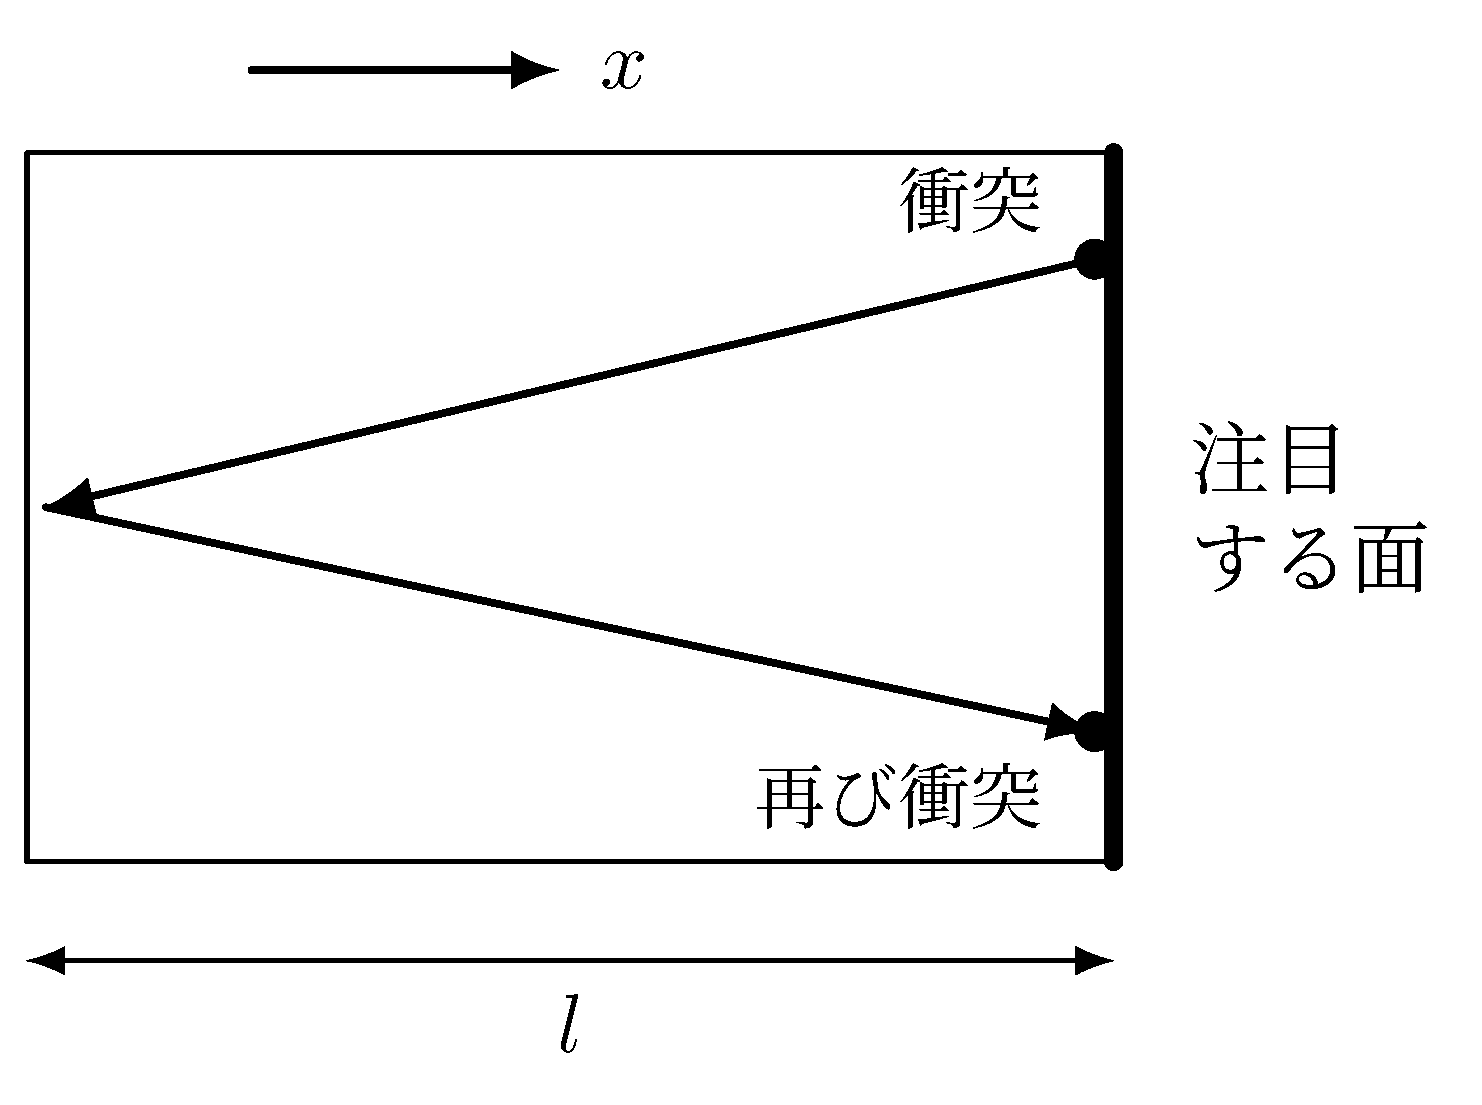
\includegraphics[keepaspectratio,width=50mm]{fig/n22_zu_ofuku.png}
\end{zuright}

\hspace{1zw}\MARU{3}では，力積を力に直す．
実際には壁はとぎれとぎれにたたかれているが，衝突の間隔が極めて短いため，一定の力が連続して作用しているように見える．
この平均の力を$\overline{F}\U{N}$とすれば，（力積）＝（平均の力）$\times$（作用した時間）より，$t\U{s}$間に与えた力積の総和を$t$で割れば$\overline{F}$が求まる．
{\gtfamily 力積と力を混同しない}こと．

\Kou{2}{\MARU{4}\ \ 気体分子運動の等方性}

\begin{zuright}{52mm}
\hspace{1zw}ここまでで得られる式には$\overline{v_x^2}$が残っているが，$x$軸をどちらに取るかは我々が勝手に決めたことであり，気体の圧力が向きによって変わるはずがない．
気体分子は容器内をランダムに飛び回るため方向性を持たず，瞬間ごと・分子ごとには$x$，$y$，$z$各軸方向の速度は異なるが，全分子について平均をとると同じ値になる．
\par
\hspace{1zw}右図のように三平方の定理$v^2=v_x^2+v_y^2+v_z^2$が成り立つので，両辺を全分子について平均すれば$\overline{v^2}=\overline{v_x^2}+\overline{v_y^2}+\overline{v_z^2}$となり，等方性と合わせて次を得る．
\zusep
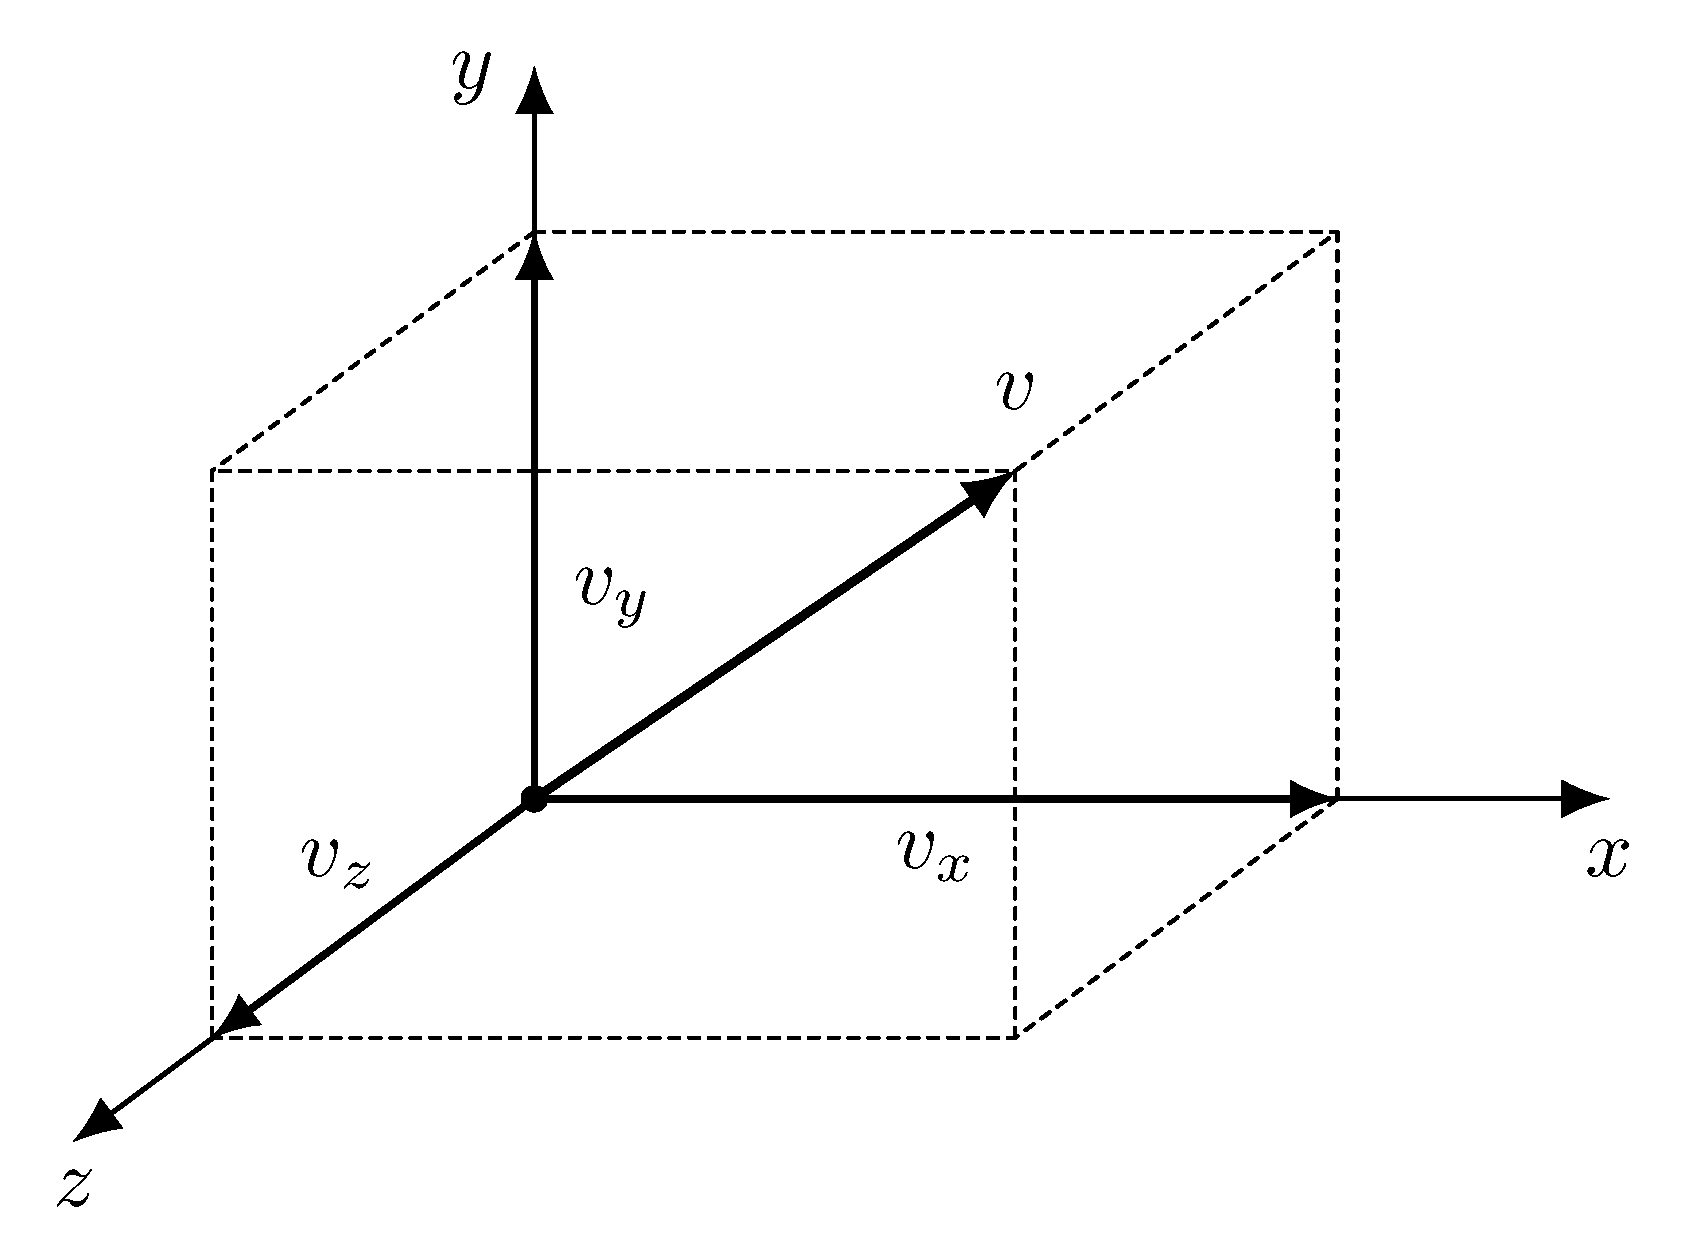
\includegraphics[keepaspectratio,width=52mm]{fig/n22_zu_seibun.png}
\end{zuright}

\noindent {\gtfamily ここではじめて$\overline{v_x^2}$を$\overline{v^2}$に書き換えられる}のがこの手順の鍵である．

\begin{matome}{気体分子運動の等方性}
 \hspace{3mm} 気体分子はランダムに飛び回るため方向性を持たず，瞬間ごと・分子ごとには$x$，$y$，$z$各軸方向の速度が異なっても，全分子について平均をとれば同じ値になる．
\AnaBD{\overline{v_x^2}=\overline{v_y^2}=\overline{v_z^2}=\frac{1}{3}\overline{v^2}}
\end{matome}

\Kou{3}{\MARU{5}\ \ 全分子ぶんを足して圧力にする}

\MARU{4}までで得られるのは「1分子が壁に及ぼす平均の力」$\dfrac{m\overline{v^2}}{3l}$である．
分子は全部で$N=nN_{\mathrm{A}}$個あり，平均すればどの分子も同じ大きさの力を及ぼすから，壁全体が受ける力はこの$N$倍である．
圧力は単位面積あたりの力だから，これを壁の面積$l^2$で割って
\[ p=\frac{1}{l^2}\times N\cdot\frac{m\overline{v^2}}{3l}=\frac{Nm\overline{v^2}}{3l^3} \]
となる．ここで$l^3$は容器の体積$V$そのものであるから，
\[ p=\frac{Nm\overline{v^2}}{3V} \]
とベルヌーイの式が得られる．
{\gtfamily 一辺$l$の立方体として計算したのに，最後は$l$が消えて体積$V$だけで書ける}ことに注意せよ．
これが「容器の形状によらず成立する」ということである（球形の容器で確かめるのが練習［19］である）．

\Kou{4}{\MARU{6}\ \ 状態方程式と比べて温度に結びつける}

ベルヌーイの式は{\gtfamily 分子の運動と圧力}を結ぶ式である．
一方，状態方程式$pV=nRT$は{\gtfamily 圧力と温度}を結ぶ式である．
したがってこの2つを組み合わせれば，{\gtfamily 分子の運動と温度}が直接結びつく．
$pV$を消去し，$Nm=nN_{\mathrm{A}}\cdot\dfrac{M}{N_{\mathrm{A}}}=nM$であることを使うと
\[ \frac{nM\overline{v^2}}{3}=nRT\qquad\Longrightarrow\qquad \sqrt{\overline{v^2}}=\sqrt{\frac{3RT}{M}} \]
となり，この節のはじめに示した二乗平均速度の式が得られる．
問題で二乗平均速度や1分子あたりの平均運動エネルギーを問われたら，ここまで進めばよい．
逆に圧力だけを問われているなら\MARU{5}で止めてよく，\MARU{6}は必要なときだけ行う．

% 加筆（2026-09-21 レビュー）：練習［21］（指定問題）が動く壁との弾性衝突をいきなり
%   要求しており，本文に前提が無かった（解答の図で初めて出てくる）．
%   第23回 23.3 の「断熱変化で温度が変わる理由」もこれである．
\Kou{5}{（発展）動いている壁との衝突}

\begin{zuright}{54mm}
\hspace{1zw}ここまでは容器が静止している場合であった．練習［21］や第23回の断熱変化で必要になるので，{\gtfamily 壁（ピストン）が動いている}場合にも触れておく．\par
\hspace{1zw}ピストンが速さ$u\U{m/s}$で近づいてくるとき，$x$方向の速さ$v_x\U{m/s}$で飛んできた分子が弾性衝突すると，はね返ったあとの速さは$v_x+2u\U{m/s}$になる．
右図のように{\gtfamily ピストンとともに動く観測者}から見れば，ピストンは静止していて分子が速さ$v_x+u$で当たってはね返るだけだからである．
\zusep
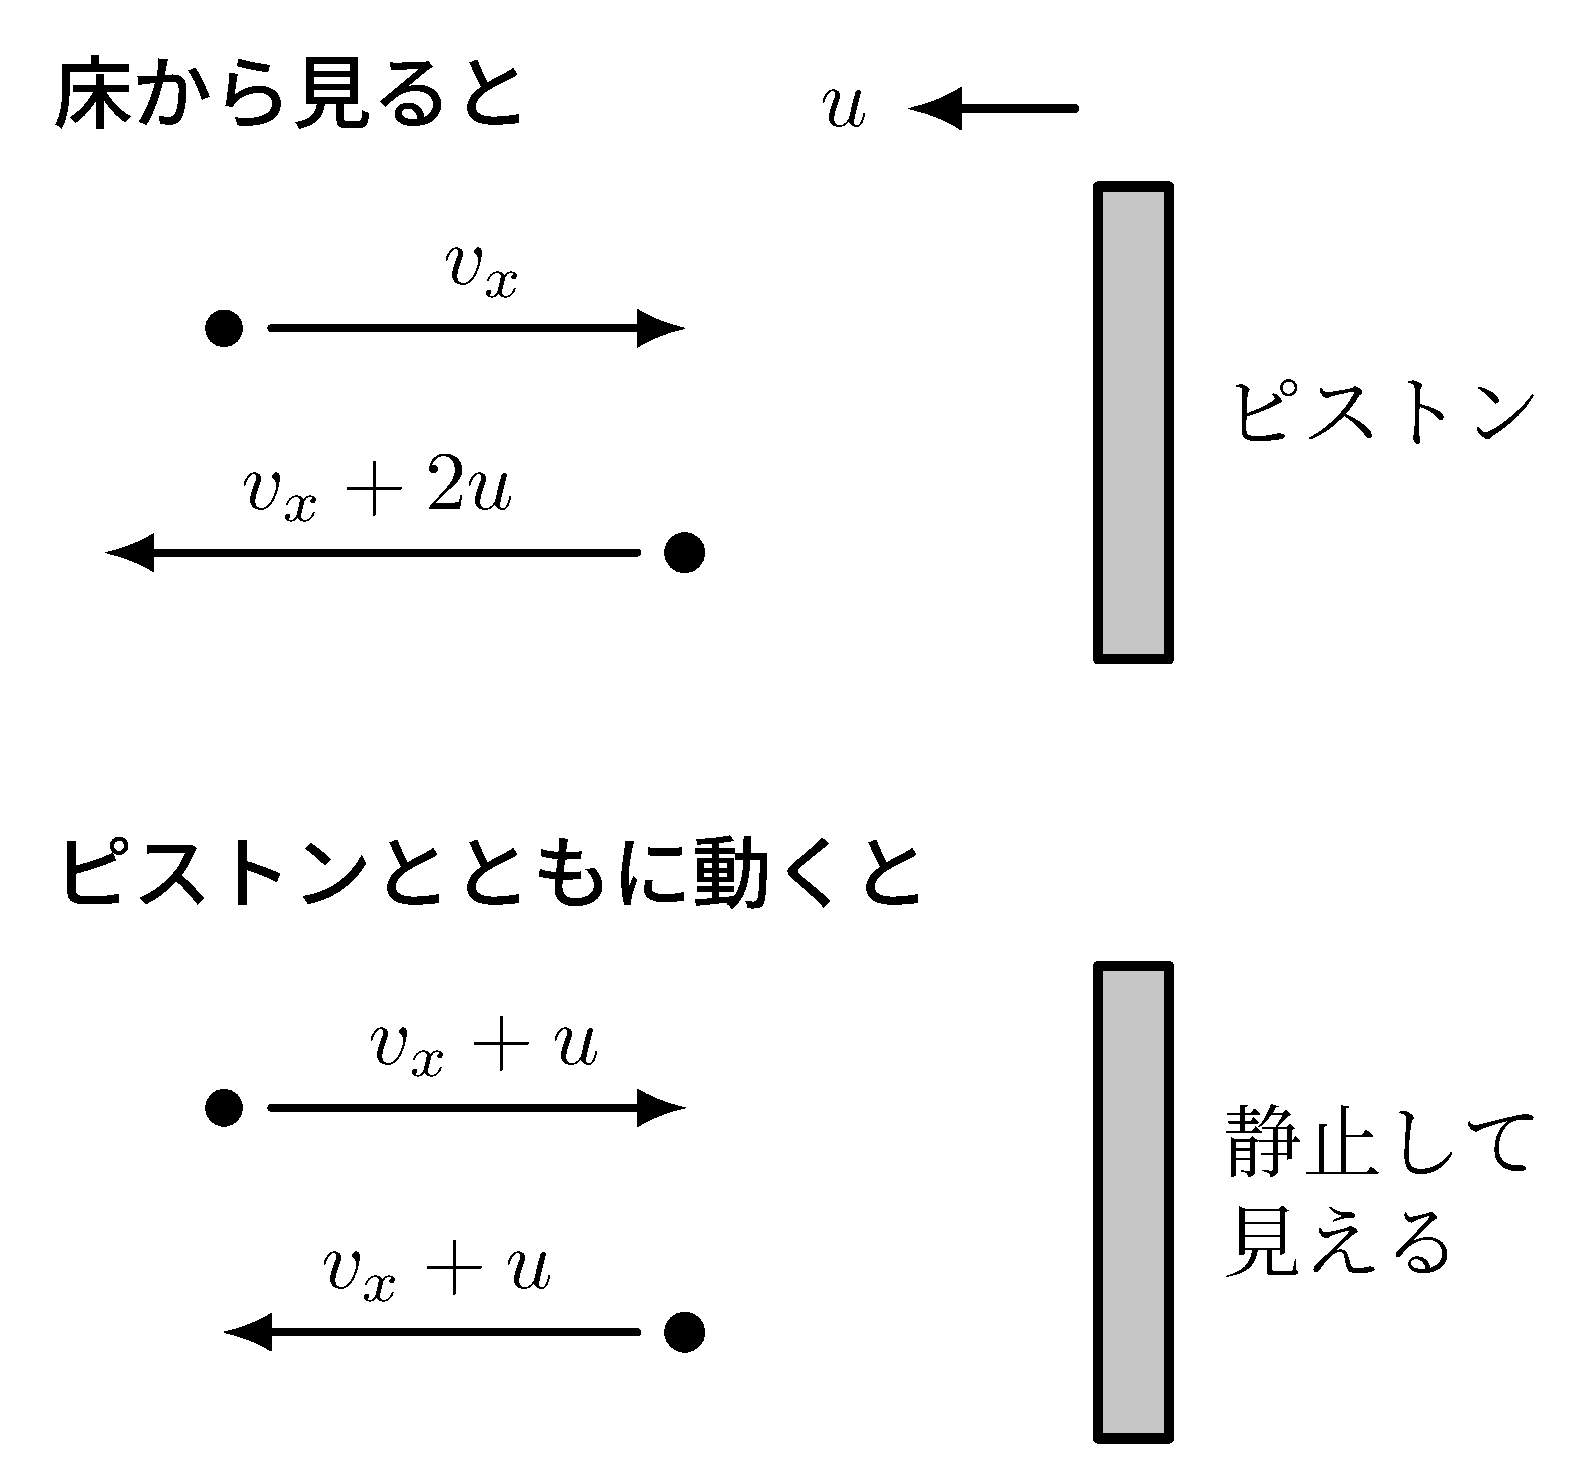
\includegraphics[keepaspectratio,width=54mm]{fig/n22_zu_kabe.png}
\end{zuright}

\noindent これを床から見た速さに直せば$(v_x+u)+u=v_x+2u$となる．
はね返り係数が$1$であることから$1=-\dfrac{v_x'-(-u)}{v_x-(-u)}$と立てて$v_x'=-(v_x+2u)$としてもよい．
すなわち{\gtfamily 近づいてくる壁にぶつかった分子は速くなり，遠ざかる壁にぶつかった分子は遅くなる}．
これが，気体を圧縮すると温度が上がり，膨張させると温度が下がることの分子的な正体である（第23回 23.3）．

%%%%%%%%%%  例題5（22.1 の直後）  %%%%%%%%%%%%%%%%%%%%
% 問題枠が大きいので，1ページに収める \bsNeed を要求すると前ページに70mm級の空白ができる．
% mondaibun は改ページで割れる設計なので，罫＋見出し＋枠の頭が出るぶんだけ確保する
% （組版チェックリスト §4）．
\bsNeed{46mm}
\begin{reidaiunit}
\begin{reidai}{気体分子運動論}
\begin{zuright}{42mm}
\hspace{1zw}気体分子の運動に関する以下の問に答えよ．ただし，速度，運動量，力積は$x$, $y$, $z$軸正の向きを正とする．\par
\hspace{1zw}一辺の長さが$l\U{m}$の立方体の容器があり，その中に$n\U{mol}$の理想気体が封入されている．気体分子1つあたりの質量を$m\U{kg}$とし，簡単のため分子同士が衝突することはないものと仮定する．\par
\hspace{1zw}今，気体分子の1つに着目し，この気体分子の持つ速度が$(v_x, v_y, v_z)\U{m/s}$だったとする．この分子が図に示した面に完全弾性衝突し，この気体分子の持つ速度が$(v_x', v_y', v_z')\U{m/s}$になったとする．
\zusep
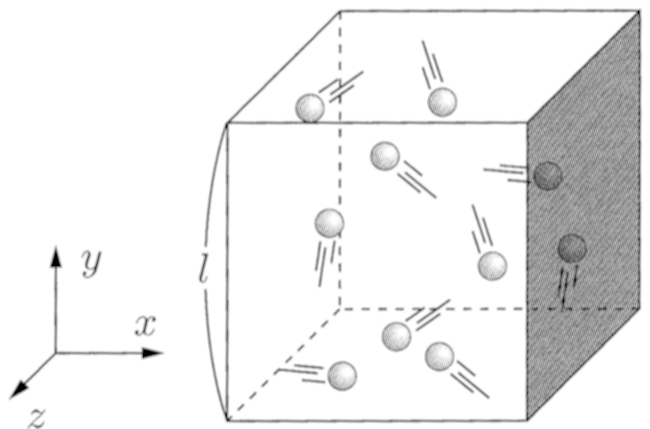
\includegraphics[keepaspectratio,width=42mm]{fig/ch15_ex5_cube.png}\\[3mm]
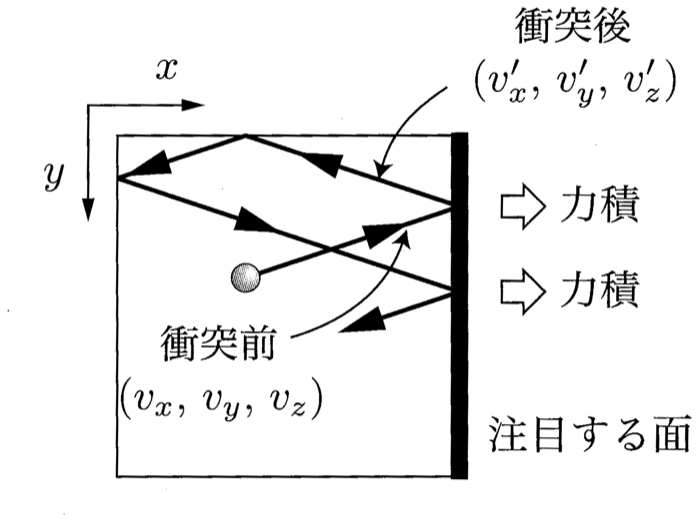
\includegraphics[keepaspectratio,width=42mm]{fig/ch15_ex5_hane.png}
\end{zuright}
\begin{komon}
\ko{1} 衝突後の速度$(v_x', v_y', v_z')$を$v_x$, $v_y$, $v_z$を用いて表せ．
\ko{2} 気体分子の持つ運動量の$x$軸方向成分の衝突1回あたりの変化$\Delta p\U{N\cdot s}$を求めよ．
\ko{3} 気体分子がこの1回の衝突により壁面に与えた力積の大きさを求めよ．
\end{komon}
\hspace{1zw}以上より，この気体分子が他の壁に衝突したとしても$x$軸方向の速度の大きさ$|v_x|\U{m/s}$は不変である．
\begin{komon}
\ko{4} この気体分子が図の面に衝突したのち再びこの面に衝突するまでにかかる時間$\tau\U{s}$を求めよ．
\ko{5} (4)を元に，この気体分子が時間$t\U{s}$の間に図の面に衝突する回数を求めよ．
\ko{6} 以上より，この気体分子が時間$t\U{s}$の間に図の面に与える力積の大きさを求めよ．
\end{komon}
\begin{zuright}{50mm}
\hspace{1zw}実際にはこの面に力（力積）が作用するのは不連続で，とぎれとぎれに作用しているが，実際には再衝突までの時間が短いために，あたかも一定の力が連続的に作用しているかのように感じられる．作用する時間を$t\U{s}$，作用する平均の力の大きさを$\overline{F}\U{N}$とする．
\zusep
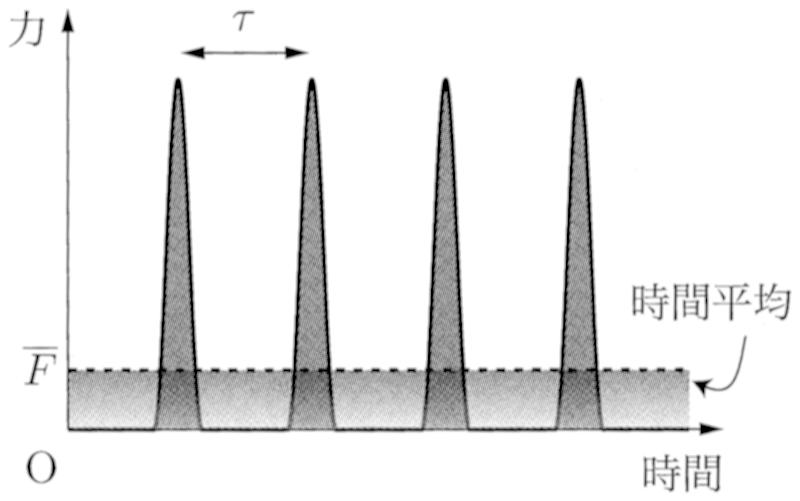
\includegraphics[keepaspectratio,width=50mm]{fig/ch15_ex5_Ft.png}
\end{zuright}
\begin{komon}
\ko{7} (6)より，この1分子が壁に作用する平均の力の大きさ$\overline{F}\U{N}$を求めよ．
\end{komon}
\hspace{1zw}さて，実際には分子ごとに分子の持つ速度は異なっている．よって分子ごとに$\overline{F}\U{N}$の値も異なるが，これを全分子に対して平均化することを考える．$x$軸方向の速度$v_x$の二乗の平均値を$\overline{v_x^2}$とおく．
\begin{komon}
\ko{8} 平均して1分子あたりがこの壁面に対して及ぼす力の大きさを求めよ．
\ko{9} 気体分子の運動は容器の形状によらずに空間に対して等方的である．このことから，$\overline{v_x^2}$, $\overline{v_y^2}$, $\overline{v_z^2}$の間に成り立つ関係式を示せ．
\ko{10} (9)より，(8)の1分子あたりの力を気体分子の持つ速度の大きさ$v\U{m/s}$の二乗平均$\overline{v^2}\U{m^2/s^2}$を用いて表せ．
\ko{11} アボガドロ数を$N_{\mathrm{A}}$として，この容器内に入っている気体分子の総数を求めよ．
\ko{12} これらより，壁に作用する全力の大きさ，および壁に作用する圧力$p\U{Pa}$を求めよ．
\ko{13} 容器の体積を$V(=l^3)\U{m^3}$とする．$pV$の値を求めよ．
\end{komon}
\hspace{1zw}理想気体であれば，気体定数$R\U{J/mol\cdot K}$，気体の温度$T\U{K}$を用いて状態方程式$pV=nRT$が成立する．
\begin{komon}
\ko{14} (13)と状態方程式を元に，気体分子の二乗平均平方根速度$\sqrt{\overline{v^2}}\U{m/s}$を，気体分子の$1\U{mol}$あたりの質量$M\U{kg/mol}$を用いて表せ．
\end{komon}
\end{reidai}

\begin{sisinE}
気体分子運動論の問題は，圧力を求めるまでの流れが決まっている．その道筋を把握しておくこと．本問はその流れを(1)から(13)まで順にたどるように作られている．

とくに混同しやすいのが「分子が受けた力積」と「分子が壁に与えた力積」，および「力積」と「力」である．前者は作用・反作用の法則で等大逆向き，後者は（力積）＝（平均の力）$\times$（作用した時間）で結ばれる．

(9)の等方性は，$x$, $y$, $z$のどの向きも同等であることから従う．三平方の定理$v^2=v_x^2+v_y^2+v_z^2$と合わせると$\overline{v_x^2}=\dfrac{1}{3}\overline{v^2}$となり，ここではじめて$\overline{v^2}$の式に書き換えられる．
\end{sisinE}

\Key{運動量の変化＝受けた力積\quad 作用・反作用で壁が受ける力積は逆向き\quad $\overline{F}t=$力積の総和\quad $\overline{v_x^2}=\frac{1}{3}\overline{v^2}$}

\begin{kaitou}
\begin{komon}
\ko{1} 図の面は$x$軸に垂直であるから，完全弾性衝突では面に平行な$y$, $z$成分は変化せず，面に垂直な$x$成分だけが符号を変える．よって，
       \[(v_x', v_y', v_z')=(-v_x, v_y, v_z)\Ans\]
\ko{2} 運動量の$x$成分の変化は，
       \[\Delta p=mv_x'-mv_x=-2mv_x\U{N\cdot s}\Ans\]
\ko{3} (2)は分子が壁から受けた力積である．作用・反作用の法則より，分子が壁に与えた力積はこれと等大逆向きの$2mv_x\U{N\cdot s}$であるから，その大きさは
       \[2m|v_x|\U{N\cdot s}\Ans\]
\ko{4} 図の面に再び衝突するには，分子は$x$軸方向に往復分の$2l\U{m}$を進まなければならない．$x$軸方向の速さは$|v_x|$のまま変化しないので，
       \[\tau=\frac{2l}{|v_x|}\U{s}\Ans\]
\ko{5} 衝突の時間間隔は$\tau$で一定であるから，時間$t\U{s}$の間の衝突回数は
       \[\frac{t}{\tau}=\frac{|v_x|t}{2l}\,[\text{回}]\Ans\]
\ko{6} 1回あたり$2m|v_x|\U{N\cdot s}$を$\dfrac{|v_x|t}{2l}$回与えるから，
       \[2m|v_x|\cdot\frac{|v_x|t}{2l}=\frac{mv_x^2t}{l}\U{N\cdot s}\Ans\]
\ko{7} （力積）＝（平均の力）$\times$（作用した時間）より$\overline{F}\cdot t=\dfrac{mv_x^2t}{l}$であるから，
       \[\overline{F}=\frac{mv_x^2}{l}\U{N}\Ans\]
\ko{8} (7)の$v_x^2$を全分子について平均すればよいから，
       \[\overline{F}=\frac{m\overline{v_x^2}}{l}\U{N}\Ans\]
\ko{9} $x$, $y$, $z$のどの向きも同等であるから，
       \[\overline{v_x^2}=\overline{v_y^2}=\overline{v_z^2}\Ans\]
\ko{10} 三平方の定理$v^2=v_x^2+v_y^2+v_z^2$の両辺を全分子で平均すると$\overline{v^2}=\overline{v_x^2}+\overline{v_y^2}+\overline{v_z^2}$となり，(9)よりこれは$3\overline{v_x^2}$に等しい．よって$\overline{v_x^2}=\dfrac{1}{3}\overline{v^2}$であるから，
       \[\overline{F}=\frac{m\overline{v^2}}{3l}\U{N}\Ans\]
\ko{11} $n\U{mol}$あるから，分子の総数は
       \[N=nN_{\mathrm{A}}\,[\text{個}]\Ans\]
\ko{12} 壁に作用する全力の大きさは，(10)を全分子分足し合わせて
       \[N\overline{F}=\frac{nN_{\mathrm{A}}m\overline{v^2}}{3l}\U{N}\Ans\]
       壁の面積は$l^2\U{m^2}$であるから，圧力は
       \[p=\frac{nN_{\mathrm{A}}m\overline{v^2}}{3l\cdot l^2}=\frac{nN_{\mathrm{A}}m\overline{v^2}}{3l^3}\U{Pa}\Ans\]
\ko{13} $V=l^3$であるから，
       \[pV=\frac{nN_{\mathrm{A}}m\overline{v^2}}{3}\left(=\frac{Nm\overline{v^2}}{3}\right)\Ans\]
       これがベルヌーイの式である．
\ko{14} (13)と$pV=nRT$を結ぶと，
       \[\frac{nN_{\mathrm{A}}m\overline{v^2}}{3}=nRT\]
       ここで$M=mN_{\mathrm{A}}\U{kg/mol}$であるから，$\dfrac{M\overline{v^2}}{3}=RT$，すなわち$\overline{v^2}=\dfrac{3RT}{M}$となる．よって，
       \Ana{\sqrt{\overline{v^2}}=\sqrt{\frac{3RT}{M}}\U{m/s}\Ans}
\end{komon}
\end{kaitou}
\end{reidaiunit}

\subsection{単原子分子理想気体の内部エネルギー}

実在する気体の中で，希ガス（$=$He,\hspace{1mm}Ne,\hspace{1mm}Arなど）のように原子そのものが単独で飛び回っているもの，すなわち分子$=$原子であるものを{\gtfamily 単原子分子}という．
これに対して，窒素や酸素のように2つの原子によって1つの分子が構成されているものは{\gtfamily 二原子分子}という．
ここでは気体のうち前者の単原子分子気体のみに着目する．

単原子分子気体の代表は上で述べた希ガスだが，希ガスは閉殻構造をとるため原子間に作用する力が非常に小さい．
そのため，実在気体でも理想気体にかなり近いことが知られている．
ここでは単原子分子であり，かつ理想気体の条件を満たす単原子分子理想気体について考え，その内部エネルギーを分子運動に基づいて算出する．

気体の内部エネルギーとは，気体が内部に蓄えることのできるエネルギーのことをいう．
気体の内部を微視的に見てみると，与えたエネルギーは気体分子が個々にもつ力学的エネルギー（$=$運動エネルギー$+$位置エネルギー）として蓄えられる．
よって，{\gtfamily 気体のもつ内部エネルギーとは気体分子のもつ力学的エネルギーの総和のことを意味する．}
% 加筆（2026-09-20）：原本はここで「力学的エネルギーの総和」とだけ述べ，位置エネルギーが
%   どこへ行ったのかを説明しないまま U=(3/2)nRT（＝運動エネルギーだけ）へ進んでいた．
ここで，{\gtfamily 理想気体では分子間にはたらく力を無視する}のであった．
力がはたらかなければ位置エネルギーも考えなくてよいから，{\gtfamily 理想気体の内部エネルギーは分子の運動エネルギーの総和だけで書ける}ことになる．

気体の内部エネルギーを一般の気体すべてについて分子運動に基づいて求めることは不可能であるが，上で述べた単原子分子理想気体の場合は容易に求めることができる．
理想気体であるなら，前に述べたベルヌーイの式や気体の二乗平均速度の式，気体の状態方程式などをすべて適用できる．
さらに，単原子分子気体においては気体分子（$=$原子）のもつエネルギーは運動エネルギーのみであり，1分子あたりの平均運動エネルギーは
\[E=\frac{1}{2}m\overline{v^2}\]
% 誤植訂正（2026-08-31，旧 physics_ch15.tex から引き継ぎ）：$v^2$ の上のバーが抜けていた．
である．これと気体の二乗平均速度の式$\overline{v^2}=\dfrac{3RT}{M}$（$M=mN_{\mathrm{A}}$）より，
\AnaBD{E=\frac{1}{2}m\cdot\frac{3RT}{mN_{\mathrm{A}}}=\frac{3}{2}\cdot\frac{R}{N_{\mathrm{A}}}T}
この式の$\dfrac{R}{N_{\mathrm{A}}}$を{\gtfamily ボルツマン定数} \mbox{\boldmath $k_{\mathrm{B}}$}という（単に$k$と書くこともある）．
% 表記の統一（2026-09-20）：原本は本文で $k$，練習・解答で $k_\mathrm{B}$ と書いていた．
ボルツマン定数は気体1分子あたりの気体定数を表すものである．
\[k_{\mathrm{B}}=\frac{R}{N_{\mathrm{A}}} \fallingdotseq 1.38\times10^{-23}\U{J/K}\]
気体の内部エネルギー$U\U{J}$はこの運動エネルギーの総和である．
気体分子の総数は$nN_{\mathrm{A}}$であるから，
\[ U=\frac{3}{2}k_{\mathrm{B}}T\times nN_{\mathrm{A}} =\mbox{\boldmath $\dfrac{3}{2}nRT$}\ \U{J}\]
と求められる．
{\gtfamily 内部エネルギーが温度だけで決まり，体積や圧力にはよらない}ことに注意せよ．

\begin{matome}{単原子分子理想気体}
 \hspace{3mm} 1分子あたりの平均運動エネルギー\hspace{11mm} $E=\dfrac{1}{2}m\overline{v^2}=\dfrac{3}{2}k_{\mathrm{B}}T$\\
 \hspace{3mm} ボルツマン定数\hspace{40mm} $k_{\mathrm{B}}=\dfrac{R}{N_{\mathrm{A}}}$\\
 \hspace{3mm} 単原子分子理想気体の内部エネルギー\hspace{8mm} $U=\dfrac{3}{2}nRT$
\end{matome}

ただし，内部エネルギーが$U=\dfrac{3}{2}nRT$となるのは{\gtfamily 単原子分子理想気体の場合のみ}である．
一般的には，理想気体の内部エネルギーは次節で述べる定積モル比熱$C_V\U{J/mol\cdot K}$を用いて
\[U=nC_VT\]
と表され，単原子分子理想気体ではこの定積モル比熱が$C_V=$\,\AnaB{$\frac{3}{2}R$}\,であるため上の式となる．
しかし，例えば窒素や酸素といった二原子分子であれば{\gtfamily 常温付近では}$C_V=\dfrac{5}{2}R$となり，内部エネルギーの式は
\[U=\frac{5}{2}nRT\]
となる．
\mbox{\boldmath $U=\dfrac{3}{2}nRT$} {\gtfamily が成立するのは単原子分子理想気体の場合のみ}であることに注意せよ．

% 加筆（2026-09-20）：3/2 と 5/2 の差がどこから来るのかが原本では説明されておらず，
%   練習［13］の参考で「回転のエネルギー」が初めて出てくる．図を添えて本文に置いた．
\begin{center}
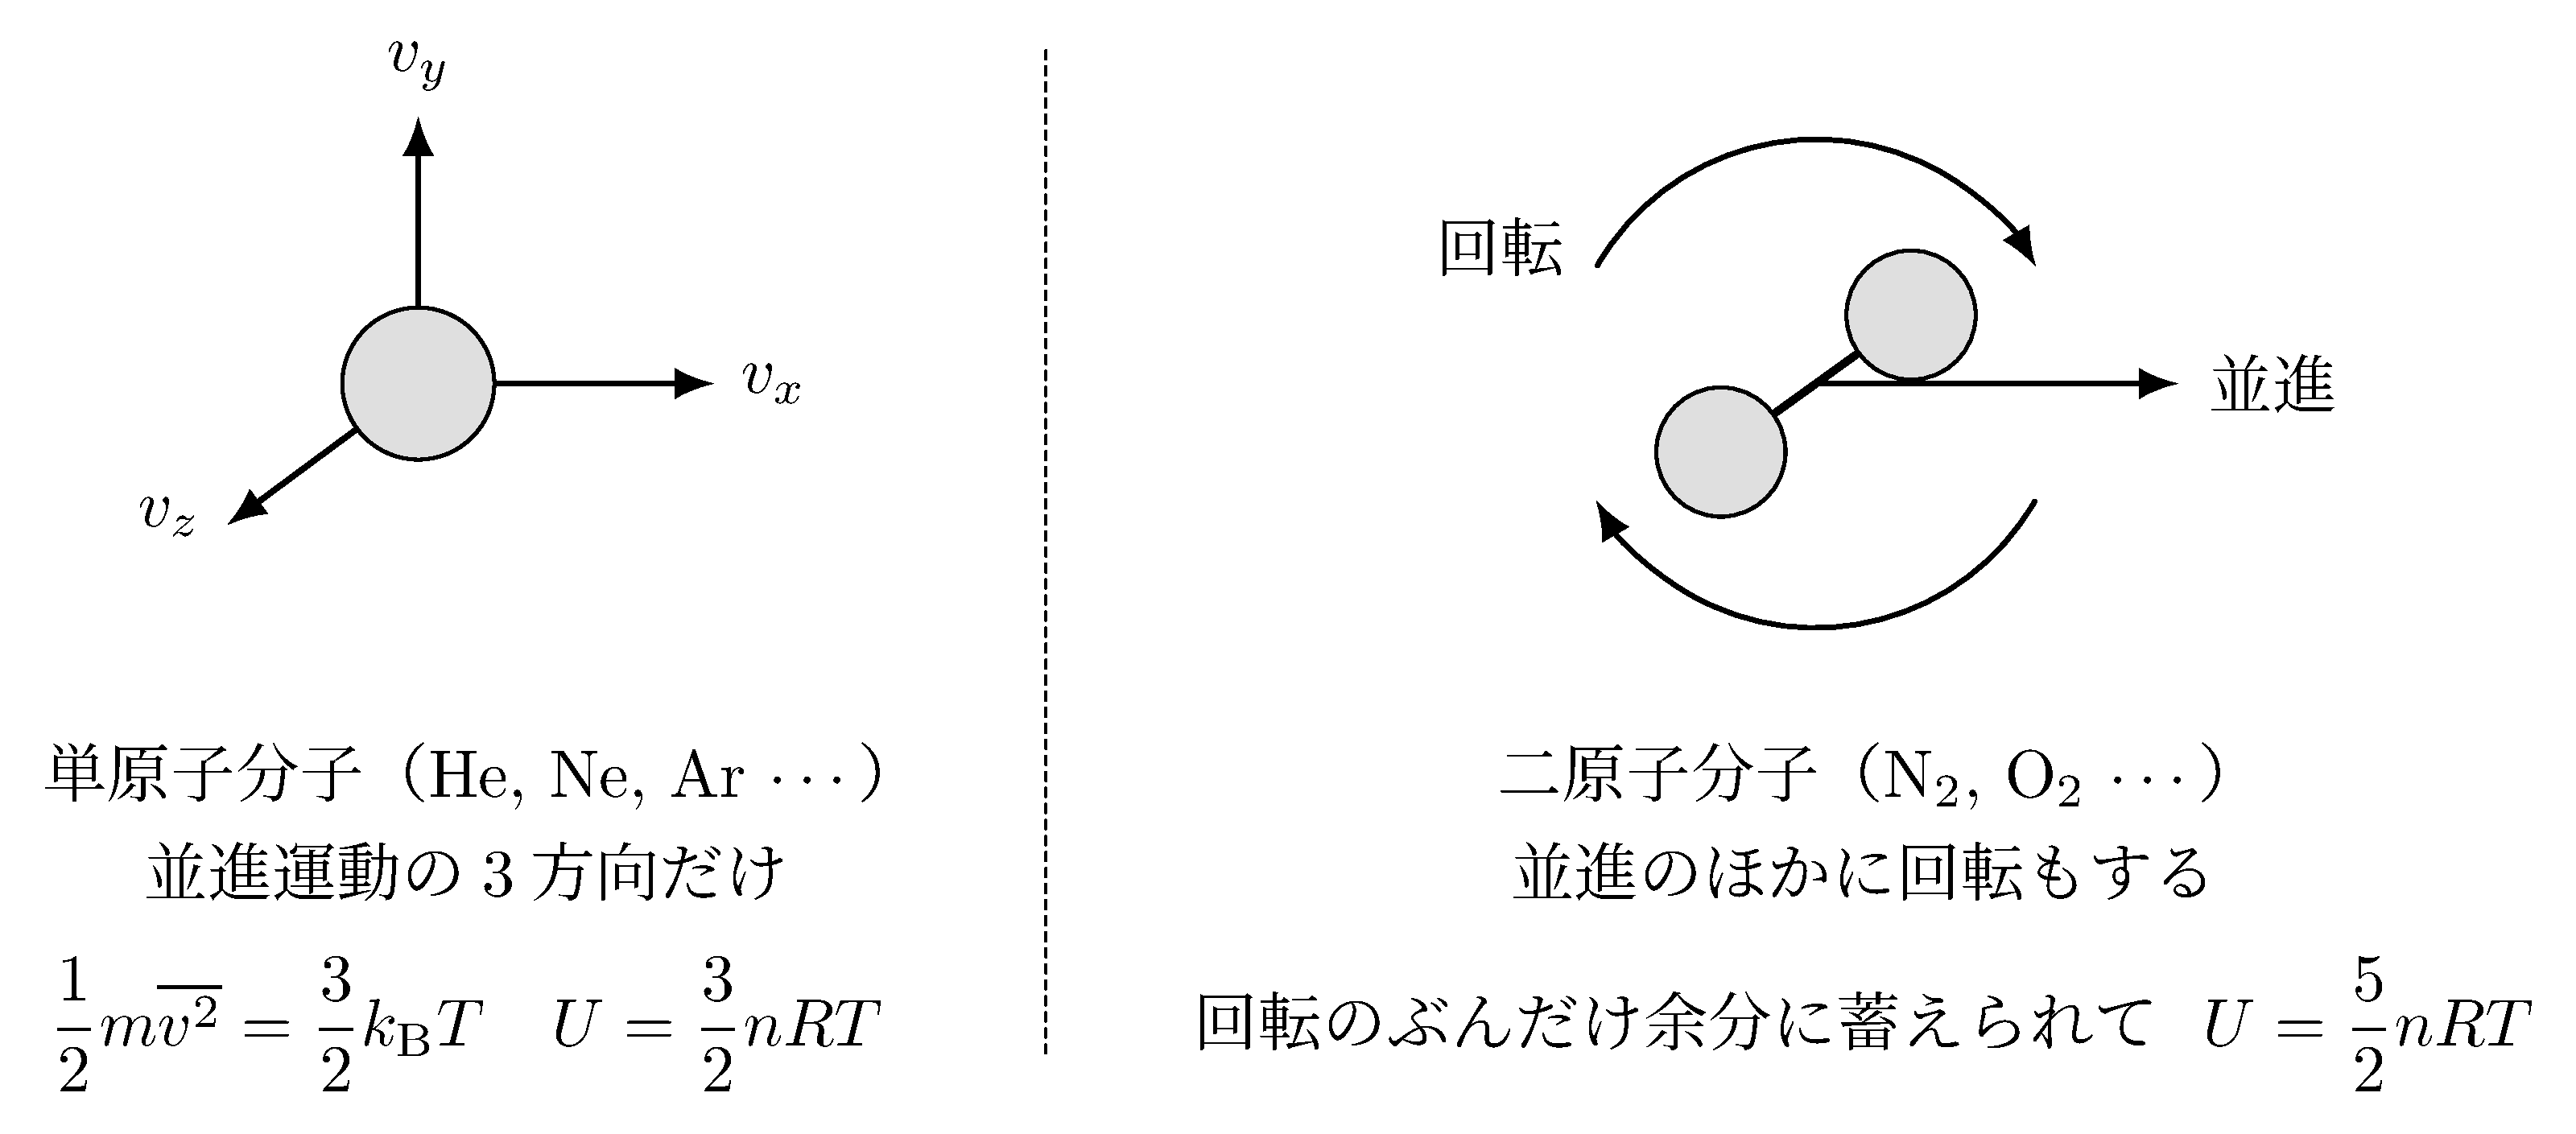
\includegraphics[keepaspectratio,width=132mm]{fig/n22_zu_bunshi.png}
\end{center}

\noindent 両者の差は，二原子分子には分子そのものの{\gtfamily 回転}という運動が加わることによる．
与えたエネルギーの一部が回転に振り分けられるため，同じ温度でも二原子分子のほうが多くのエネルギーを蓄える．
% 訂正（2026-09-21 レビュー）：二原子分子では回転の運動エネルギーもあるので，
%   3/2 k_B T を単に「平均運動エネルギー」と呼ぶと意味があいまいになる．
一方，1分子あたりの{\gtfamily 平均並進運動エネルギー}（分子の重心の運動によるぶん）$E=\dfrac{1}{2}m\overline{v^2}=\dfrac{3}{2}k_{\mathrm{B}}T$のほうは，導出にベルヌーイの式と状態方程式しか使っていないので，{\gtfamily 単原子分子でなくても成立する．}
二原子分子ではこれに回転のぶんが加わるので，1分子がもつエネルギーの平均は$\dfrac{3}{2}k_{\mathrm{B}}T$より大きい．
「内部エネルギーを分子数で割る」という求め方は単原子分子のときしか使えないので区別すること．

%%%%%%%%%%  例題6（22.2 の直後）  %%%%%%%%%%%%%%%%%%%%
\bsNeed{72mm}
\begin{reidaiunit}
\begin{reidai}{単原子分子理想気体の内部エネルギー}
\begin{zuright}{50mm}
\hspace{1zw}容積が$V_1$, $V_2\U{m^3}$の断熱容器$\mathrm{A}$, $\mathrm{B}$をコック$\mathrm{K}$のついた細管でつなぐ．$\mathrm{K}$を閉じた状態で単原子分子理想気体を$\mathrm{A}$には圧力$P_1\U{Pa}$，温度$T_1\U{K}$で，$\mathrm{B}$には圧力$P_2\U{Pa}$，温度$T_2\U{K}$でそれぞれ注入した．$\mathrm{K}$を開いて十分時間を経過させるときの変化について，気体定数を$R\U{J/mol\cdot K}$として以下の問に答えよ．
\zusep
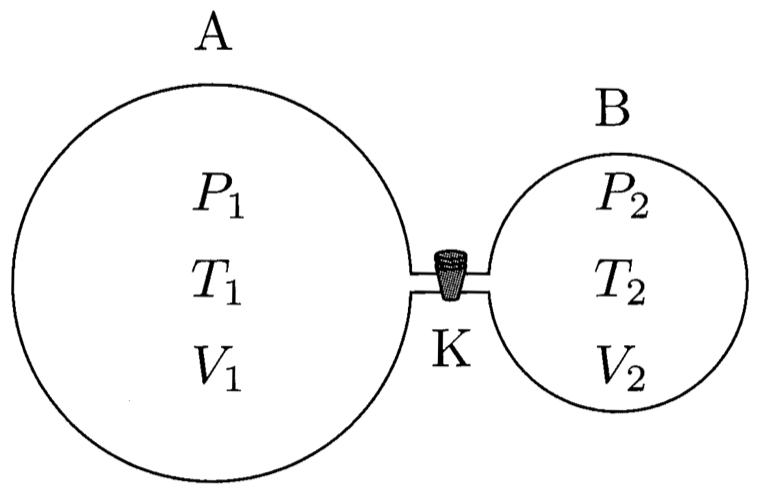
\includegraphics[keepaspectratio,width=50mm]{fig/ch15_ex6_cock.png}
\end{zuright}
\vspace{-\medskipamount}
\begin{komon}
\ko{1} $\mathrm{K}$を開く前に$\mathrm{A}$，$\mathrm{B}$に入っていた気体のモル数$n_1$, $n_2\U{mol}$を求めよ．
\ko{2} この状態変化で気体の内部エネルギーの総和は保存される．このことを利用して十分時間が経過した後の気体の温度$T\U{K}$を求めよ．
\ko{3} 十分時間が経過した後の容器内の気体の圧力$P\U{Pa}$を求めよ．
\end{komon}
\end{reidai}

\begin{sisinE}
容器は断熱されているので外界と熱のやり取りをせず（$Q_{\mathrm{in}}=0$），容器全体の体積も変わらないので気体は外界に対して仕事もしない（$W_{\mathrm{out}}=0$）．よって熱力学第一法則より内部エネルギーの総和は変化しない，というのが(2)の「保存される」の中身である．

あとは単原子分子理想気体の内部エネルギーが$U=\dfrac{3}{2}nRT$と書けることを使えばよい．$nRT=PV$であることに注意すると，$U=\dfrac{3}{2}PV$と書き直せて計算がかなり楽になる．
\end{sisinE}

\Key{単原子分子理想気体\quad $\Rightarrow$\quad 内部エネルギー$U=\dfrac{3}{2}nRT=\dfrac{3}{2}PV$}

\begin{kaitou}
\begin{komon}
\ko{1} それぞれの状態方程式$P_1V_1=n_1RT_1$, $P_2V_2=n_2RT_2$より，
       \[n_1=\frac{P_1V_1}{RT_1}\U{mol},\quad n_2=\frac{P_2V_2}{RT_2}\U{mol}\Ans\]
\ko{2} 単原子分子理想気体であるから，$\mathrm{K}$を開く前の内部エネルギーの総和は，$nRT=PV$を用いて
       \[U=\frac{3}{2}n_1RT_1+\frac{3}{2}n_2RT_2=\frac{3}{2}(P_1V_1+P_2V_2)\]
       である．$\mathrm{K}$を開いた後は全体が温度$T\U{K}$の一様な状態になるから，そのときの内部エネルギーは
       \[U'=\frac{3}{2}(n_1+n_2)RT\]
       である．内部エネルギーの総和は保存されるので$U'=U$，すなわち
       \[(n_1+n_2)RT=P_1V_1+P_2V_2\]
       これに(1)を代入して，
       \[\left(\frac{P_1V_1}{T_1}+\frac{P_2V_2}{T_2}\right)T=P_1V_1+P_2V_2\]
       よって，
       \Ana{T=\frac{T_1T_2(P_1V_1+P_2V_2)}{P_1V_1T_2+P_2V_2T_1}\U{K}\Ans}
\ko{3} 十分時間が経過した後の気体は，体積$V_1+V_2\U{m^3}$，物質量$n_1+n_2\U{mol}$，温度$T\U{K}$であるから，状態方程式は
       \[P(V_1+V_2)=(n_1+n_2)RT\]
       である．(2)で得た$(n_1+n_2)RT=P_1V_1+P_2V_2$を代入して，
       \[P=\frac{P_1V_1+P_2V_2}{V_1+V_2}\U{Pa}\Ans\]
\end{komon}
\end{kaitou}
\end{reidaiunit}

\subsection{状態変化と$P$-$V$図}

気体の状態を変化させる（$=$圧力，体積，温度などを変化させる）際，圧力$P\U{Pa}$を縦軸に，体積$V\U{m^3}$を横軸に取ったグラフを用いてその変化の様子を表すと便利なことが多い．
この変化図を$P$-$V$図という．

% 整形（2026-09-20）：原本はこの5項目を数式モードの中に和文を入れて組んでいた
%   （$\MARU{1} \hspace{2mm} 水平な直線上での変化は定圧変化を表す．$）．箇条書きに直した．
\begin{zuright}{50mm}
\hspace{1zw}$P$-$V$図上での特徴を以下にまとめる．
\begin{komon}
\item[{\makebox[1.9zw][r]{\MARU{1}}}] 水平な直線上での変化は\,\AnaB{定圧変化}\,を表す．
\item[{\makebox[1.9zw][r]{\MARU{2}}}] 鉛直な直線上での変化は\,\AnaB{定積変化}\,を表す．
\item[{\makebox[1.9zw][r]{\MARU{3}}}] 等温変化は$P=\dfrac{nRT}{V}\propto\dfrac{1}{V}$であるから，\,\AnaB{双曲線}\,（反比例のグラフ）となる．
\end{komon}
\zusep

\includegraphics[keepaspectratio,width=50mm]{text_p73_fig1.png}
\end{zuright}
\begin{komon}
% 訂正（2026-09-20）：原本は「上側にある双曲線上に乗っている点の方が温度が高い」だが，
%   「上側」だけでは同じ双曲線上の点どうしと区別できない．PV=nRT に即した言い方に改めた．
\item[{\makebox[1.9zw][r]{\MARU{4}}}] $PV=nRT$より，{\gtfamily 一定量の気体では}$PV$の値が大きい点ほど温度が高い．すなわち{\gtfamily 原点から遠い（右上の）双曲線に乗っている点ほど温度が高い．}
% 訂正（2026-09-20）：原本は「P-V図で囲む面積が気体のやりとりした仕事を表す」．
%   何と何で囲むのか・符号がどうなるのかが書かれていなかったので補った．
\item[{\makebox[1.9zw][r]{\MARU{5}}}] {\gtfamily グラフと$V$軸で囲まれた部分の面積}が，その変化で気体が外界にした仕事$W_{\mathrm{out}}\U{J}$を表す．右向き（膨張）なら正，左向き（圧縮）なら負である．
\end{komon}

\noindent ただし\MARU{5}は，各瞬間に気体の圧力が定まっているようなゆっくりした変化（準静的過程）についての話である（第23回 23.1）．
\MARU{5}を実際に計算する方法は，定積変化・定圧変化については次節で，圧力が変化する一般の場合については第23回で扱う．

%%%%%%%%%%  例題7（22.3 の直後）  %%%%%%%%%%%%%%%%%%%%
\bsNeed{58mm}
\begin{reidaiunit}
\begin{reidai}{$P$-$V$図}
\begin{zuright}{44mm}
\hspace{1zw}一定量の理想気体の状態を図の矢印の順に静かに変化させた．$\mathrm{A}$での体積が$V_0\U{m^3}$であるときについて，この状態変化を$P$-$V$図上での変化に書き直せ．ただし，グラフには$\mathrm{A}$, $\mathrm{B}$, $\mathrm{C}$, $\mathrm{D}$点を明示し，変化の方向に矢印をつけること．
\zusep
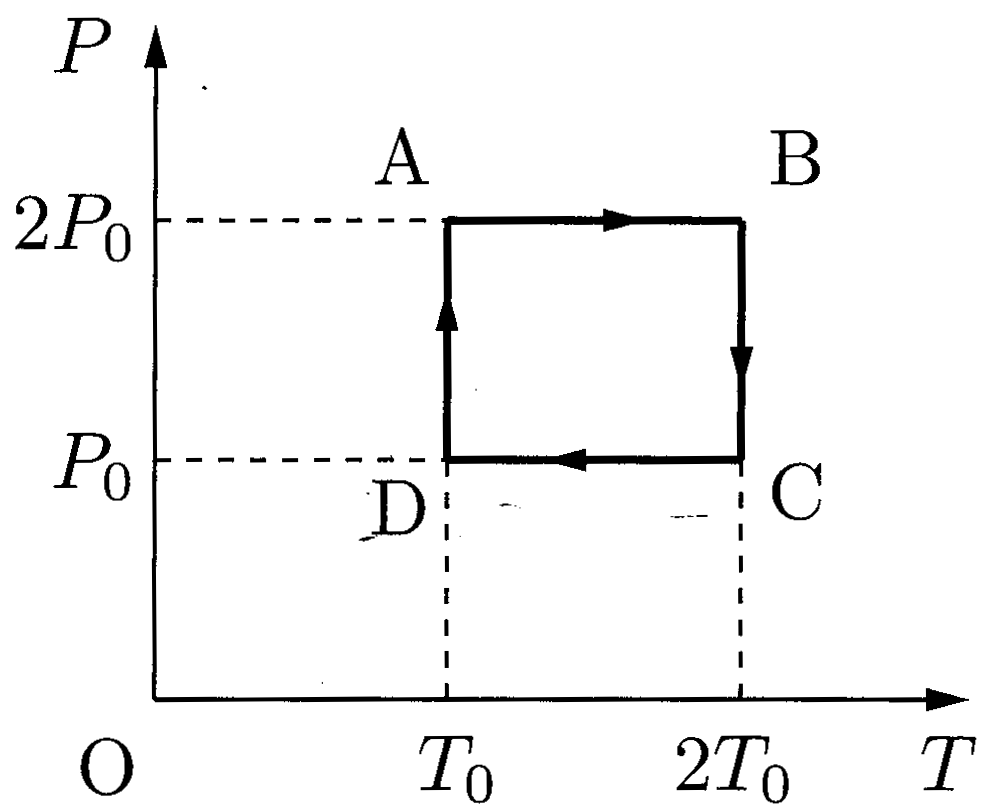
\includegraphics[keepaspectratio,width=44mm]{fig/ch15_ex7_pt.png}
\end{zuright}
\end{reidai}

\begin{sisinE}
例えば温度が変化しないならば，$PV=nRT$, $P'V'=nRT$のかわりに$PV=P'V'$を考えるなど，変化しない状態量を状態方程式から除いて考えると楽である．

まず4点それぞれの体積を状態方程式から求めて位置を決め，そのあとで各変化が定圧変化・等温変化のどちらであるかを見て，直線で結ぶか双曲線で結ぶかを決めればよい．
\end{sisinE}

\Key{各点の状態方程式で体積を出す $\Rightarrow$ 変化中に一定な量を見て線の種類を決める}

\begin{kaitou}
\hspace{1zw}気体の物質量を$n\U{mol}$，気体定数を$R\U{J/mol\cdot K}$とする．与えられた図より，各点の圧力と温度は
\[\mathrm{A}(T_0,\,2P_0),\quad \mathrm{B}(2T_0,\,2P_0),\]
\[\mathrm{C}(2T_0,\,P_0),\quad \mathrm{D}(T_0,\,P_0)\]
である．$\mathrm{A}$での体積が$V_0$であるから，$\mathrm{A}$での状態方程式より
\[2P_0V_0=nRT_0\qquad \text{すなわち}\quad nR=\frac{2P_0V_0}{T_0}\]
となる．これを用いて各点の体積を求めると，
\[\mathrm{B}:2P_0V_{\mathrm{B}}=nR\cdot 2T_0\ \ \text{より}\ \ V_{\mathrm{B}}=2V_0\]
\[\mathrm{C}:P_0V_{\mathrm{C}}=nR\cdot 2T_0\ \ \text{より}\ \ V_{\mathrm{C}}=4V_0\]
\[\mathrm{D}:P_0V_{\mathrm{D}}=nR\cdot T_0\ \ \text{より}\ \ V_{\mathrm{D}}=2V_0\]
となる．\par
\hspace{1zw}次に各変化を見る．
\begin{komon}
\ko{1} $\mathrm{A}\to\mathrm{B}$は圧力が$2P_0$のまま変化しないので{\gtfamily 定圧変化}であり，$P$-$V$図上では$P=2P_0$の水平な直線上を$V=V_0\to 2V_0$まで変化する．
\ko{2} $\mathrm{B}\to\mathrm{C}$は温度が$2T_0$のまま変化しないので{\gtfamily 等温変化}であり，$PV=nR\cdot 2T_0=4P_0V_0$（一定）となる．すなわち$P$-$V$図上では双曲線$P=\dfrac{4P_0V_0}{V}$の上を$V=2V_0\to 4V_0$まで変化する．
\ko{3} $\mathrm{C}\to\mathrm{D}$は圧力が$P_0$のまま変化しないので{\gtfamily 定圧変化}であり，$P=P_0$の水平な直線上を$V=4V_0\to 2V_0$まで変化する．
\ko{4} $\mathrm{D}\to\mathrm{A}$は温度が$T_0$のまま変化しないので{\gtfamily 等温変化}であり，$PV=nRT_0=2P_0V_0$（一定）となる．すなわち双曲線$P=\dfrac{2P_0V_0}{V}$の上を$V=2V_0\to V_0$まで変化する．
\end{komon}
\hspace{1zw}以上をまとめると，求める$P$-$V$図は次のようになる．
\begin{center}
% 穴埋め版（生徒用）では答のグラフを軸だけの図に差し替える．
% 2枚は同じ画素寸法なので，貼付幅が同じなら両版のページ送りは揃う．
\ifbsAnaume
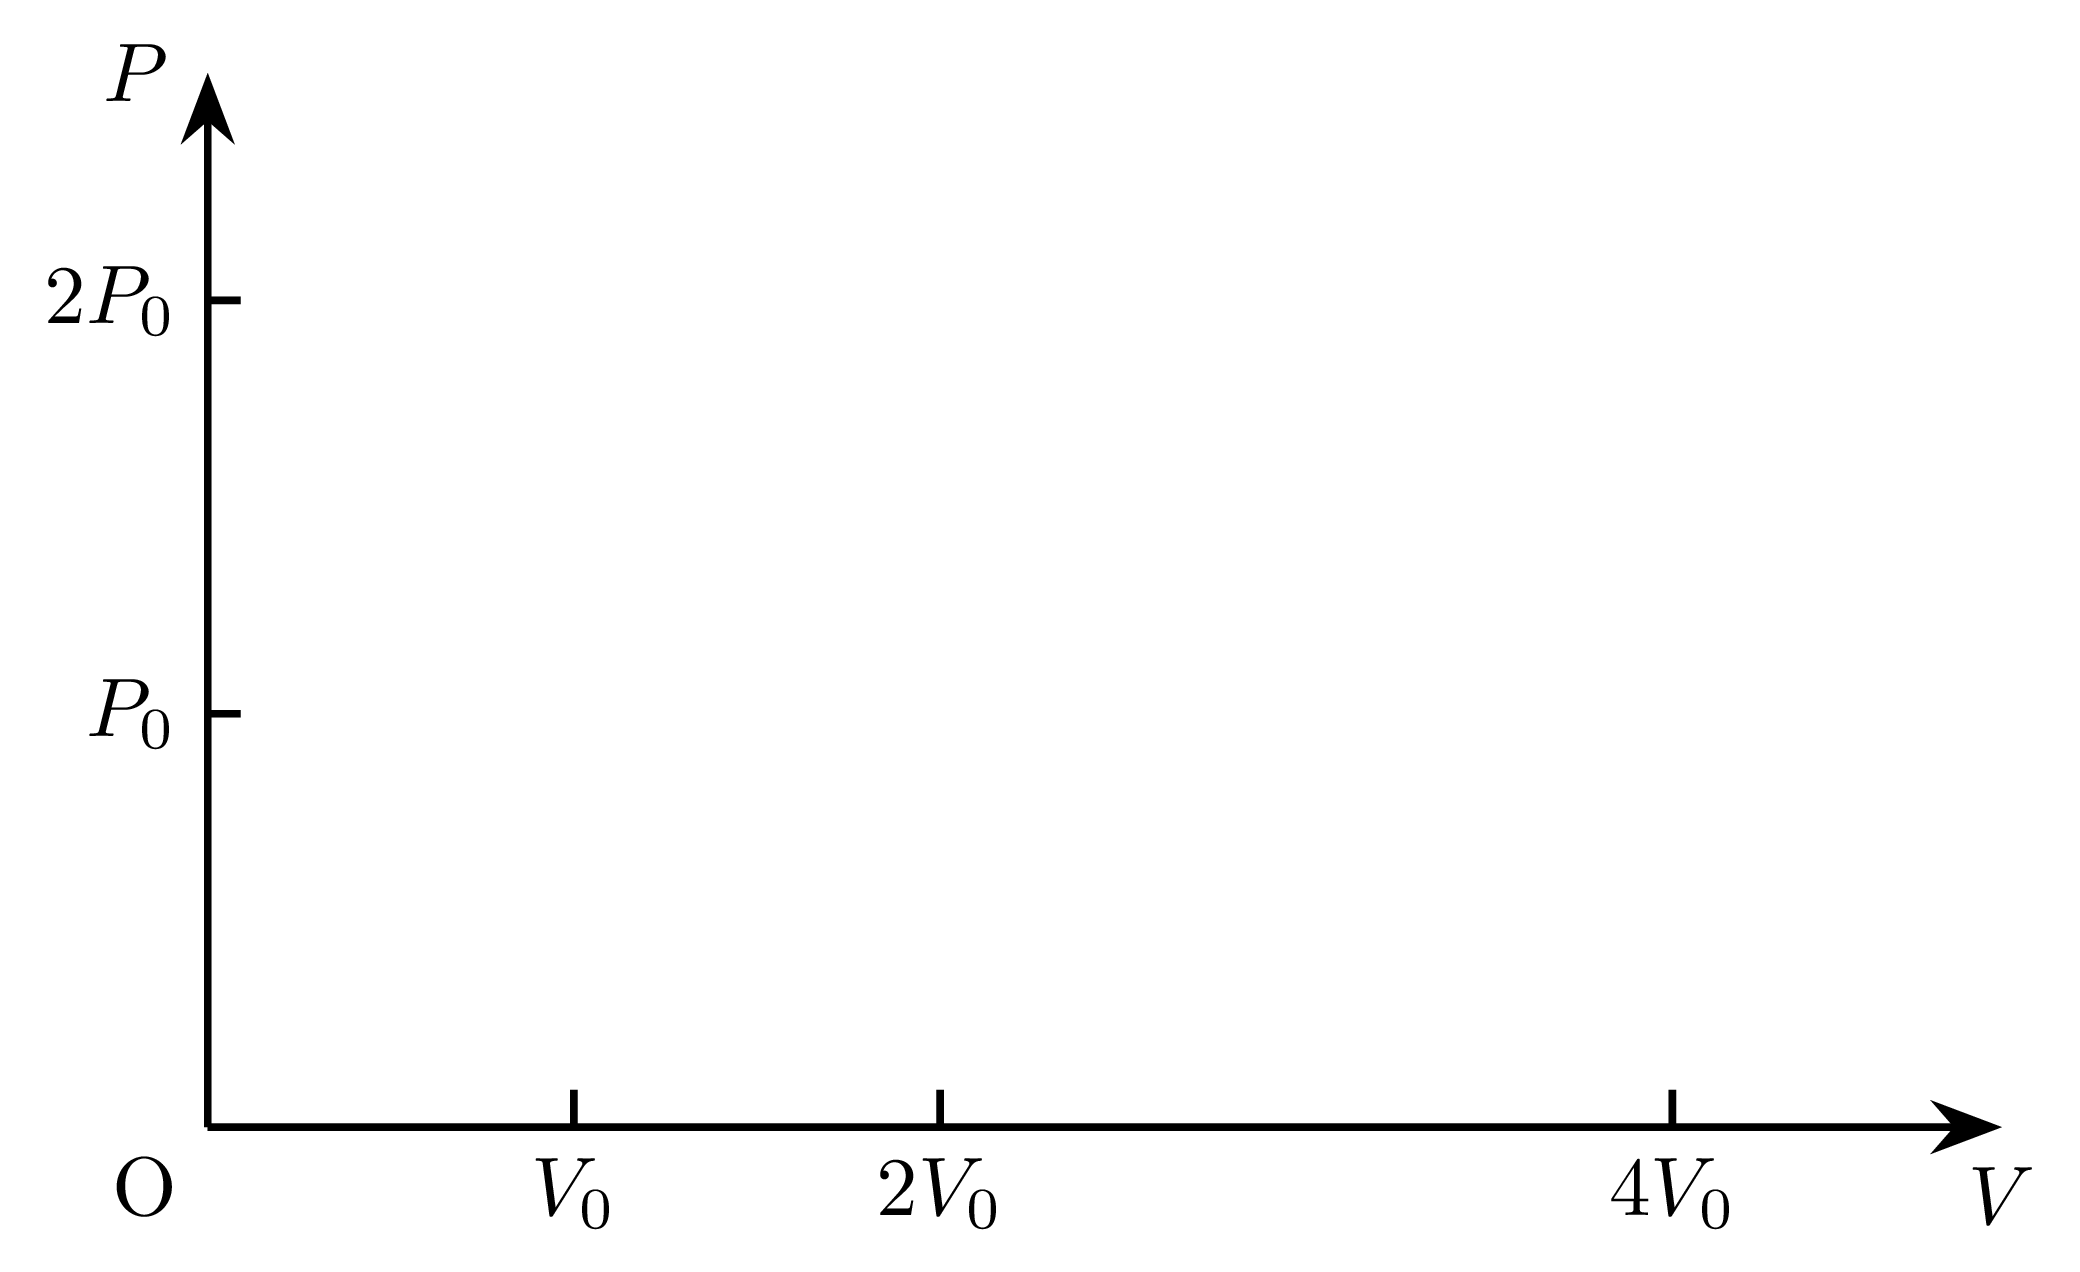
\includegraphics[keepaspectratio,width=76mm]{fig/ch15_ex7_pv_blank.png}
\else
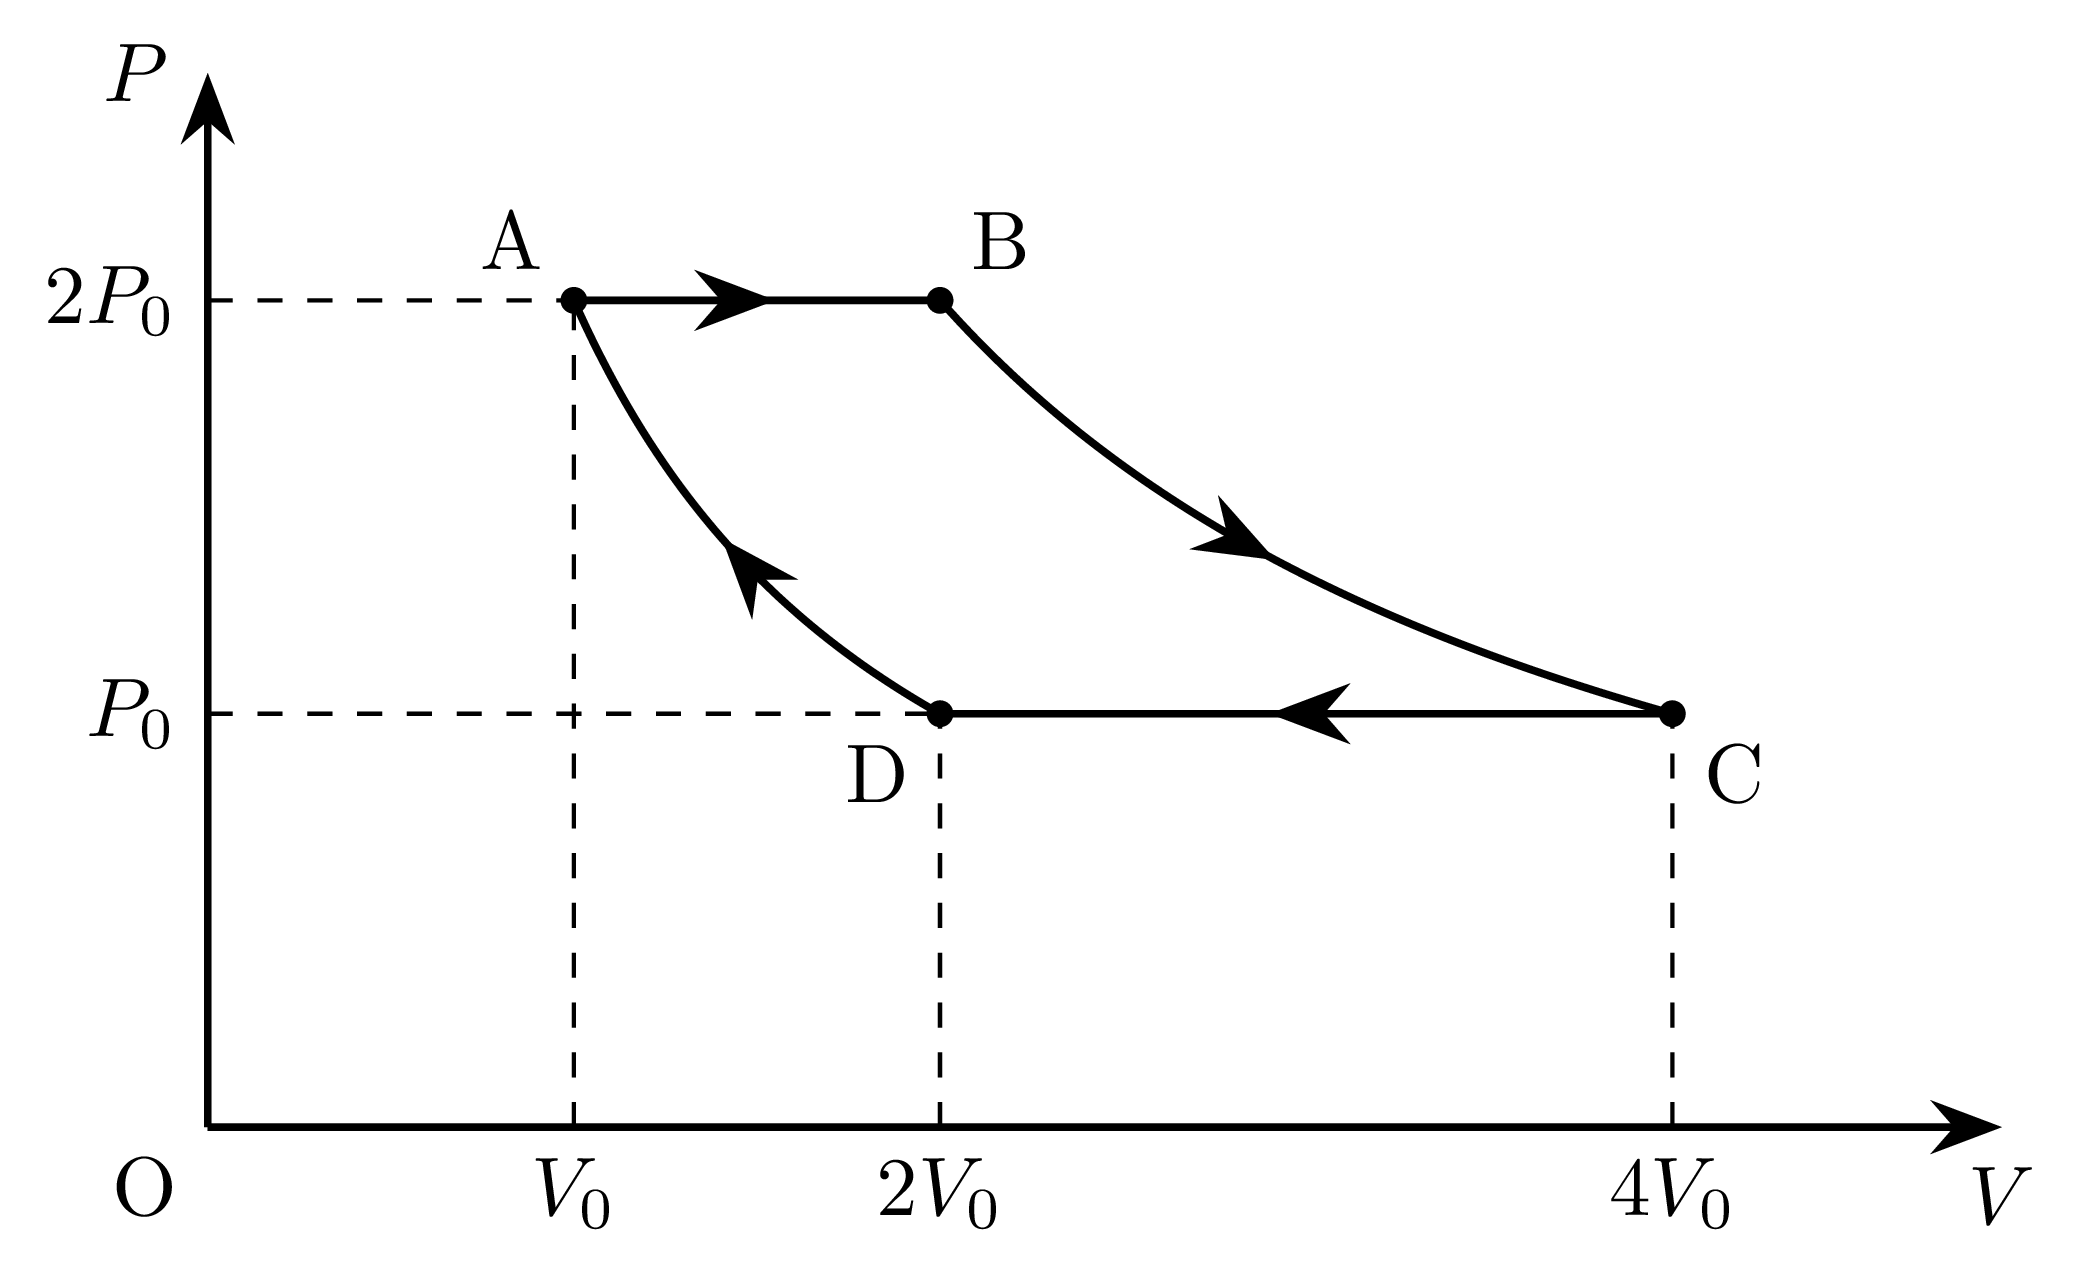
\includegraphics[keepaspectratio,width=76mm]{fig/ch15_ex7_pv.png}
\fi
\end{center}
\hspace*{\fill}\Ans
\end{kaitou}
\end{reidaiunit}

\subsection{定積モル比熱と定圧モル比熱}

通常の物質に加えるべき熱量は，その物質の比熱を$c\U{cal/g\cdot K}$，物質の質量を$m\U{g}$，上昇させる温度を$\Delta T\U{K}$として$Q=mc\Delta T\U{cal}$で与えられた．
% 誤植訂正（2026-09-20）：原本はこの式の単位を [J] としているが，c が [cal/g・K]，m が [g]
%   なら Q は [cal] である（[J] にするなら熱の仕事当量 J を掛ける）。
しかし気体を加熱する場合，気体の量は$\U{g}$ではなく$\U{mol}$で，また加える熱量も$\U{cal}$ではなく$\U{J}$を用いた方が便利である．
{\gtfamily そこで，気体の比熱を，$1\U{mol}$の気体を$1\U{K}$だけ温度上昇させるのに必要な熱量として定義する．}
これを{\gtfamily モル比熱}という．
モル比熱が$C\U{J/mol\cdot K}$のとき，$n\U{mol}$の気体の温度を$\Delta T\U{K}$だけ上昇させるのに必要な熱量$Q\U{J}$は
\AnaBD{Q=nC\Delta T}
で与えられる．

比熱はその物体に対してどのように熱を与えるかによって変化する．
気体の場合，
\Kou{1}{体積を一定に保ったまま温度を上げる（定積変化）}
\Kou{2}{圧力を一定に保ったまま温度を上げる（定圧変化）}
の2つの熱の与え方が特に重要で，これらの場合の気体のモル比熱をそれぞれ{\gtfamily 定積モル比熱} \mbox{\boldmath $C_V$} {\gtfamily $\U{J/mol\cdot K}$，定圧モル比熱}\mbox{\boldmath $C_P$}{\gtfamily $\U{J/mol\cdot K}$}という．

$C_V$と$C_P$は気体の種類によって値が違うが，理想気体の場合は必ず
\AnaBD{C_P-C_V=R}
の関係式を満たす．
これを{\gtfamily マイヤーの関係式}という．
{\gtfamily 同じ温度だけ上げるのに，定圧のほうが定積より余分に熱が要る}ことを意味しており，その理由は次節で確かめる．

\begin{matome}{定積モル比熱・定圧モル比熱}
 \hspace{3mm} 定積条件で温度を$\Delta T\U{K}$上昇させるのに必要な熱\hspace{5mm} $Q=nC_V\Delta T\U{J}$\\
 \hspace{3mm} 定圧条件で温度を$\Delta T\U{K}$上昇させるのに必要な熱\hspace{5mm} $Q=nC_P\Delta T\U{J}$\\
 \hspace{3mm} 理想気体であれば気体の種類によらずマイヤーの関係式$C_P-C_V=R$が成立
\end{matome}

\subsection{内部エネルギーの変化と熱力学第一法則の使い方}

気体の出入りがない（モル数が一定）場合の状態変化を考えよう．
この場合に重要となる物理量は，初めの状態および終わりの状態での{\gtfamily 圧力，体積，温度}と，エネルギーに関しては変化中の{\gtfamily 吸熱量，仕事，内部エネルギー変化}となる．
圧力，体積，温度は状態方程式により，これらのうち2つが分かっていれば残りの1つも決定される．
エネルギーについても，熱力学第一法則より3つの値のうち2つが分かれば残りの1つを求めることができる．

\Kou{1}{内部エネルギーの変化 $\varDelta U$}

前節で述べたように，$n\U{mol}$の理想気体の内部エネルギーは定積モル比熱を用いて$U=nC_VT$と表される（単原子分子理想気体なら$C_V=\frac{3}{2}R$）．
したがってその変化量は
\AnaBD{\varDelta U=nC_V\varDelta T}
である．
$C_V$は「定積」モル比熱という名前だが，{\gtfamily この式は定積変化に限らず，あらゆる状態変化について成立する．}
なぜなら，{\gtfamily 理想気体の内部エネルギーは温度だけで決まり，体積や圧力にはよらない}からである．
温度変化さえ分かれば，その変化が定積であろうと定圧であろうと$\varDelta U$は同じ式で計算できる．

\Kou{2}{気体が外界にした仕事 $W_{\mathrm{out}}$}

前節の\MARU{5}で述べたように，$W_{\mathrm{out}}$は$P$-$V$図のグラフと$V$軸で囲まれた部分の面積である．
この回で扱う2つの場合については，面積が単純な図形になるのですぐ計算できる．
\begin{komon}
\item[{\makebox[1.9zw][r]{\MARU{1}}}] {\gtfamily 定積変化}では体積が変化しない．$P$-$V$図は鉛直な線分で，$V$軸との間に面積を持たないから
      \[W_{\mathrm{out}}=0\]
      である．{\gtfamily 気体の仕事のやり取りは体積変化に伴って起こる}ということを押さえておこう．
\item[{\makebox[1.9zw][r]{\MARU{2}}}] {\gtfamily 定圧変化}では圧力が$P$のまま一定である．$P$-$V$図は水平な線分で，$V$軸との間の面積は縦$P$・横$\varDelta V$の長方形だから
      \AnaBD{W_{\mathrm{out}}=P\varDelta V}
      である．膨張（$\varDelta V>0$）なら正，圧縮（$\varDelta V<0$）なら負となる．
\end{komon}
圧力が変化しながら膨張する一般の場合は，長方形では済まないので積分が必要になる．これは第23回で扱う．

\Kou{3}{熱力学第一法則の使い方}

第21回で述べたように，熱力学第一法則は
\[Q_{\mathrm{in}}=\varDelta U+W_{\mathrm{out}}\]
の形で用いるのであった．
以上の3つを組み合わせると，定積変化と定圧変化については次のようになる．

% 加筆（2026-09-20）：マイヤーの関係式が天下りにならないよう，定積加熱と定圧加熱を
%   並べた図を置いた。力のつり合いの式（PS=P_0S）にも作用図を添えてある。
\begin{center}
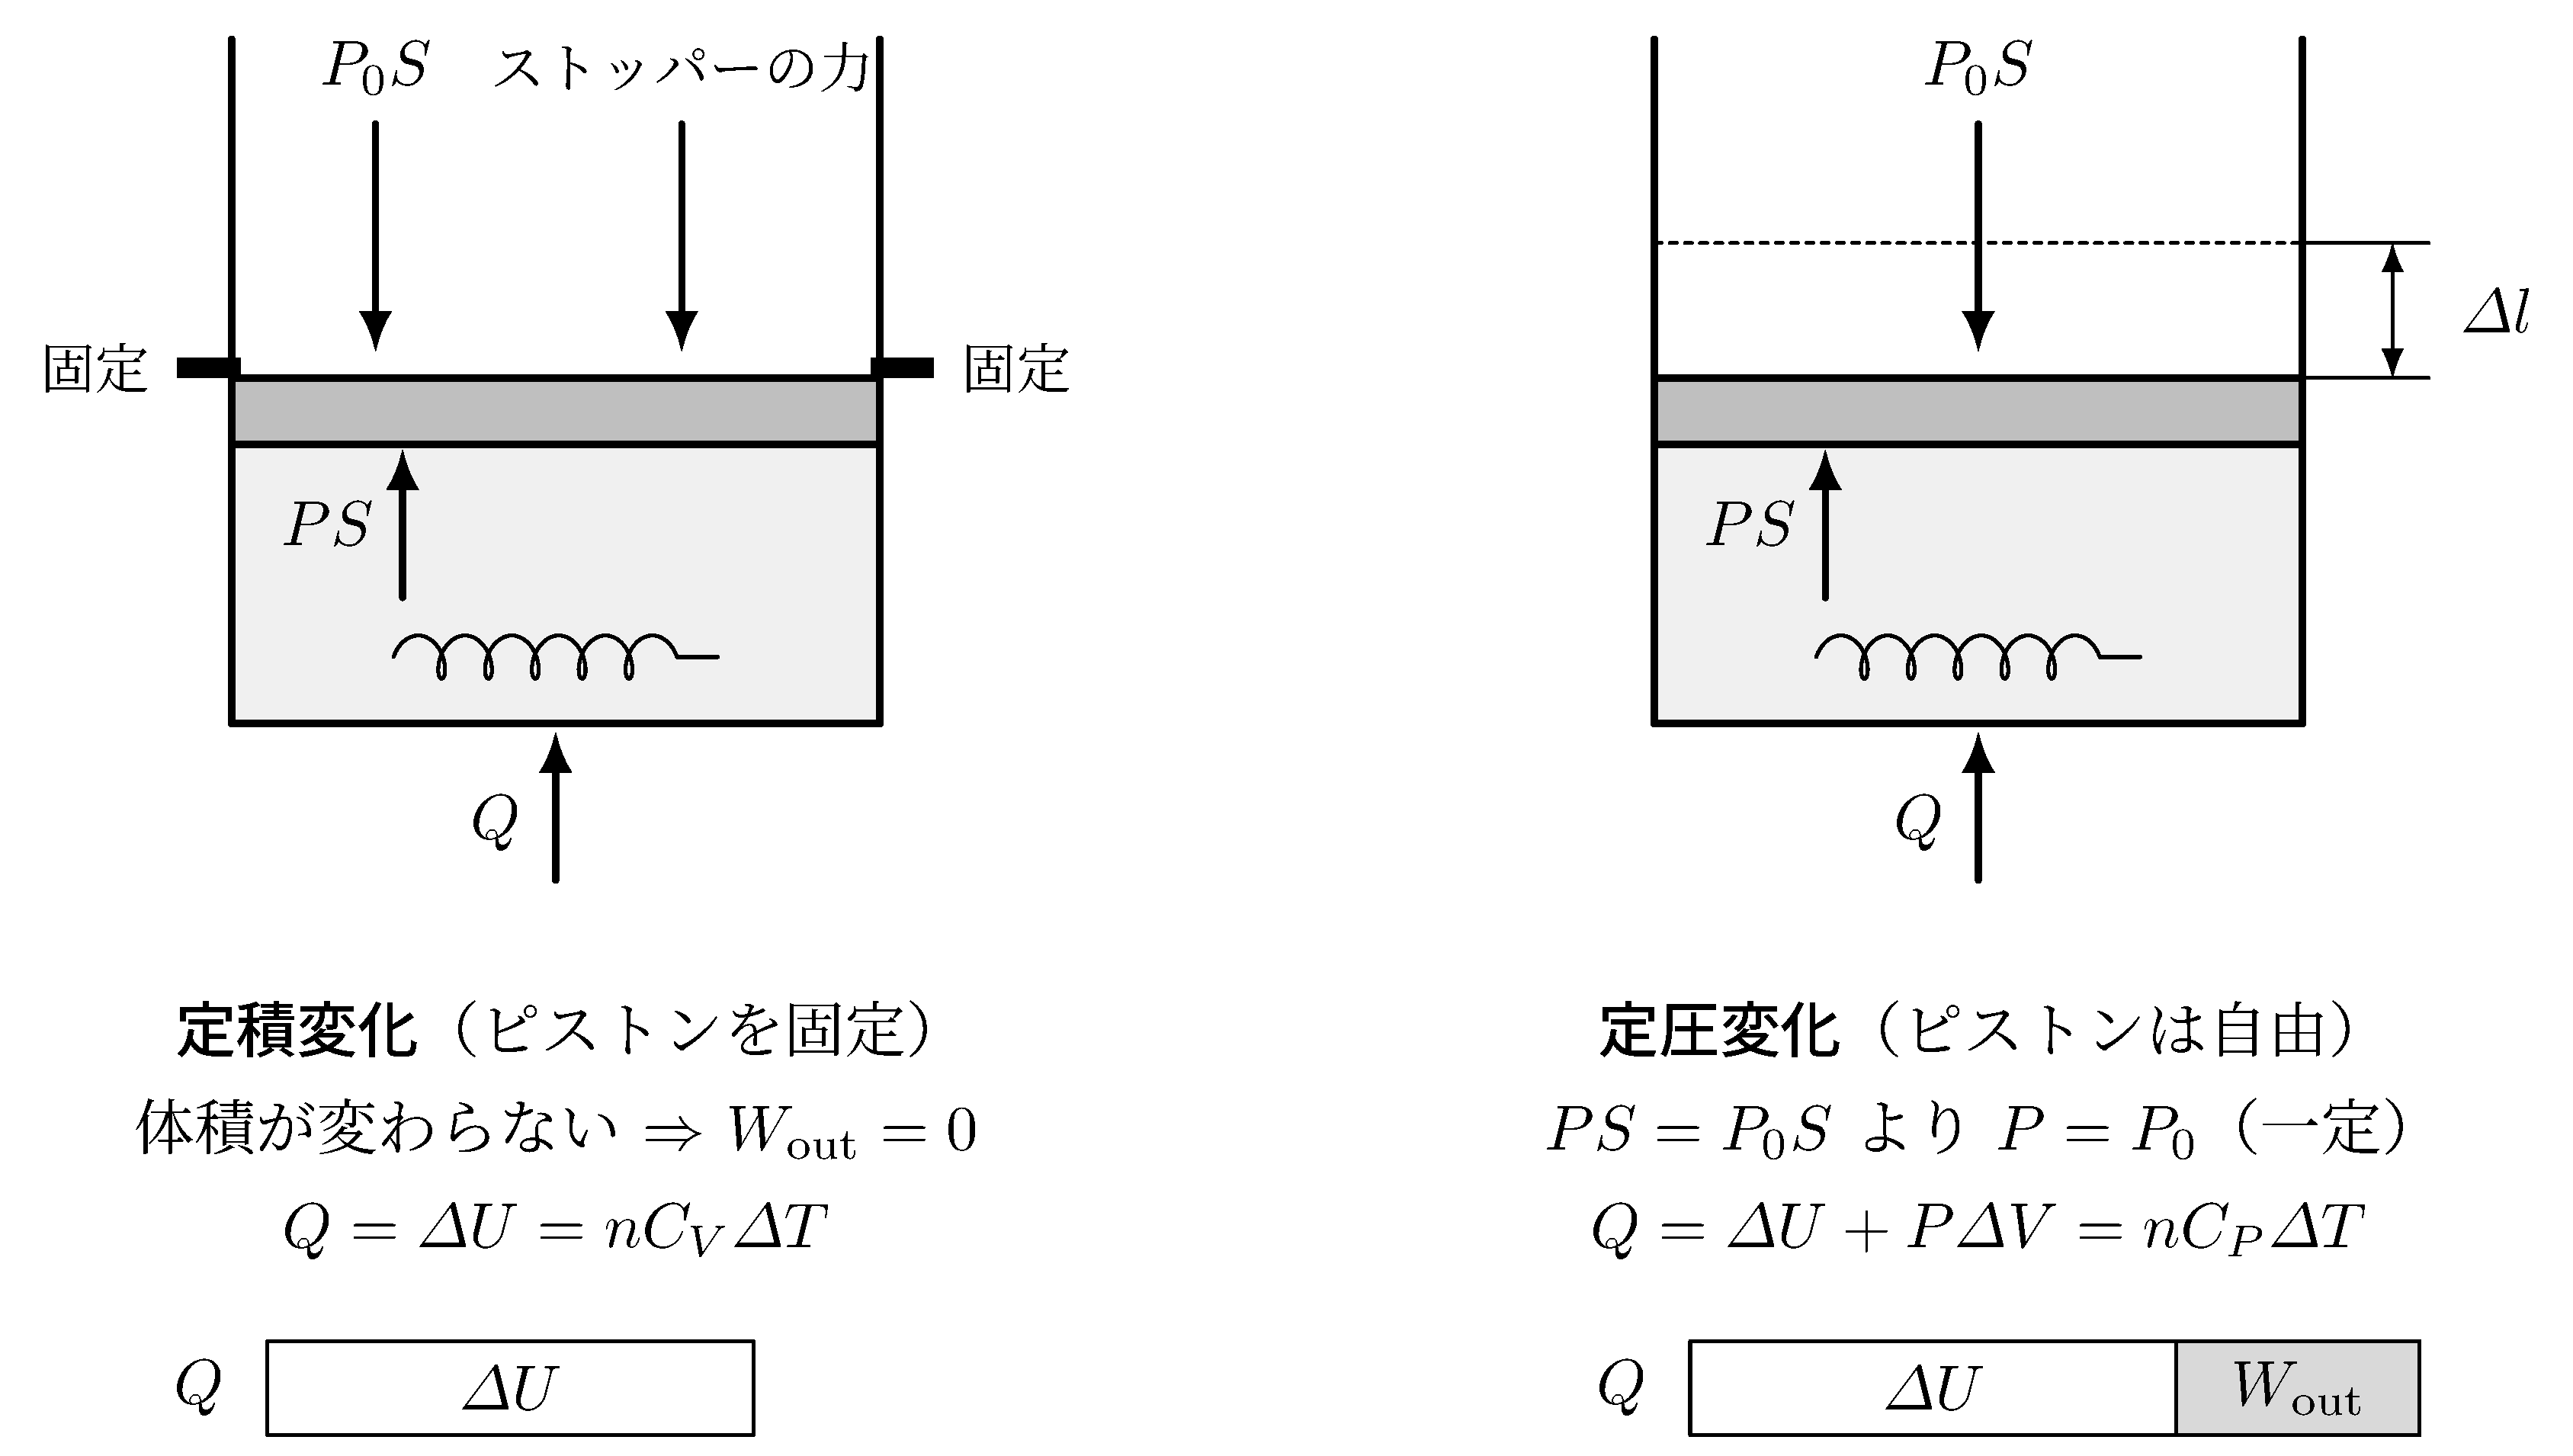
\includegraphics[keepaspectratio,width=150mm]{fig/n22_zu_teiseki.png}
\end{center}

\noindent 定積変化ではピストンを固定しているので，加熱して気体の圧力$P$が大気圧$P_0$より大きくなってもピストンは動かない（その差はストッパーが受け持つ）．
体積が変わらないので気体は仕事をせず，加えた熱がすべて内部エネルギーになるから$Q=nC_V\varDelta T$であり，これが{\gtfamily 定積モル比熱$C_V$の物理的意味}である．
一方，定圧変化では気体が膨張してピストンを押し上げるため，加えた熱の一部が仕事として外へ出ていく．
同じ$\varDelta T$を得るのに$P\varDelta V=nR\varDelta T$だけ余分な熱が必要であり，これがマイヤーの関係式$C_P-C_V=R$の正体である．

\begin{matome}{気体の状態変化の解き方}
 \hspace{3mm} \underline{\gtfamily 状態方程式}\hspace{8mm} $PV=nRT$\\[1mm]
 \hspace{3mm} \underline{\gtfamily 熱力学第一法則}\hspace{4mm} $Q_{\mathrm{in}}=\varDelta U+W_{\mathrm{out}}$\\[0.5mm]
 \hspace{8mm} 気体が外界から{\gtfamily された}仕事$W_{\mathrm{in}}$で与えられていたら$W_{\mathrm{out}}=-W_{\mathrm{in}}$と読み替える\\[1mm]
 \hspace{3mm} \underline{$\varDelta U\U{J}$：内部エネルギーの変化}\hspace{4mm} $\varDelta U=nC_V\varDelta T$\\[0.5mm]
 \hspace{8mm} 状態変化の種類にかかわらずこの式で表せる（単原子分子理想気体では$C_V=\frac{3}{2}R$）\\[1mm]
 \hspace{3mm} \underline{$W_{\mathrm{out}}\U{J}$：気体が外界にした仕事}\hspace{4mm} $P$-$V$図のグラフと$V$軸で囲む面積\\[1mm]
 \hspace*{5mm}\begin{tabular}{l@{\hspace{5mm}}l@{\hspace{5mm}}l@{\hspace{5mm}}l}
 状態変化 & 特徴 & $W_{\mathrm{out}}$ & $Q_{\mathrm{in}}$\\[0.5mm]
 定積変化 & $V$一定 & $0$                  & $nC_V\varDelta T$\\
 定圧変化 & $P$一定 & $P\varDelta V$       & $nC_P\varDelta T$\\
 等温変化 & $T$一定 & （第23回）           & $\varDelta U=0$ より $Q_{\mathrm{in}}=W_{\mathrm{out}}$\\
 断熱変化 & $Q_{\mathrm{in}}=0$ & $-\varDelta U$ & $0$
 \end{tabular}
\end{matome}

%%%%%%%%%%  例題8（22.5 のまとめ枠の直後。原本の【例題9】）  %%%%%%%%%%%%%%%%%%%%
\bsNeed{76mm}
\begin{reidaiunit}
\begin{reidai}{定積変化（$C_V$の物理的意味）}
\begin{zuright}{52mm}
\hspace{1zw}図のように一様な断面積を持つシリンダーに定積モル比熱が$C_V\U{J/mol\cdot K}$の理想気体を$n\U{mol}$封入し，ピストンの位置を固定して動かないようにした．\par
\hspace{1zw}最初，この気体の温度は$T_0\U{K}$，圧力は$P_0\U{Pa}$であった．
\zusep
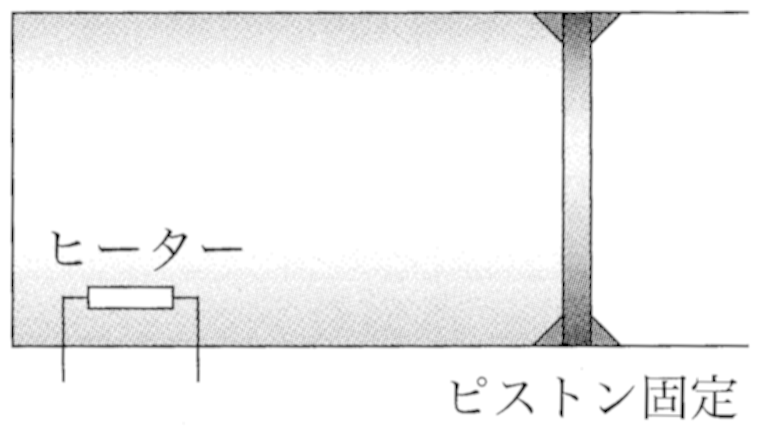
\includegraphics[keepaspectratio,width=52mm]{fig/ch16_ex9_cyl.png}
\end{zuright}
\hspace{1zw}シリンダー内にはヒーターが取り付けてあり，気体に対して熱を与えることができる．シリンダーおよびピストンは断熱材で出来ており，ヒーターによって与えた熱が大気に拡散することはないものとする．

\hspace{1zw}この状態から気体に熱をゆっくりと与え，気体の温度が$\Delta T\U{K}$だけ上昇したところで加熱を止めた．気体定数を$R\U{J/mol\cdot K}$として以下の問に答えよ．
\begin{komon}
\ko{1} この状態変化を$P$-$V$図で表せ．
\ko{2} この変化において気体が外界に対してした仕事$w\U{J}$を求めよ．
\ko{3} この変化における気体の内部エネルギーの増加$\Delta U\U{J}$およびヒーターによって加えた熱量$Q\U{J}$を求めよ．
\end{komon}
\end{reidai}

\begin{sisinE}
ピストンが固定されているので体積は変化しない．体積が変わらなければ気体は仕事をやり取りしないから，加えた熱はすべて内部エネルギーの増加になる．これが「定積モル比熱$C_V$の物理的意味」である．

$\Delta U=nC_V\Delta T$は定積変化に限らずあらゆる状態変化で成立する式であるが，$Q=nC_V\Delta T$の方は定積変化でしか成立しない．本問はその二つがたまたま一致する場合である．
\end{sisinE}

\Key{状態方程式 $PV=nRT$\quad $\Delta U=nC_V\Delta T$\quad 定積なら$W_{\mathrm{out}}=0$\quad $Q_{\mathrm{in}}=\Delta U+W_{\mathrm{out}}$}

\begin{kaitou}
\begin{komon}
\ko{1} 体積が変化しないので，$P$-$V$図は$V$軸に垂直な線分となる．初めの状態の状態方程式$P_0V_0=nRT_0$より体積は$V_0=\dfrac{nRT_0}{P_0}\U{m^3}$，終状態の状態方程式$P_1V_0=nR(T_0+\Delta T)$より圧力は$P_1=\dfrac{T_0+\Delta T}{T_0}P_0\U{Pa}$であり，加熱したので圧力は上昇する．よって$P$-$V$図は次図．
       \begin{center}
       \ifbsAnaume
       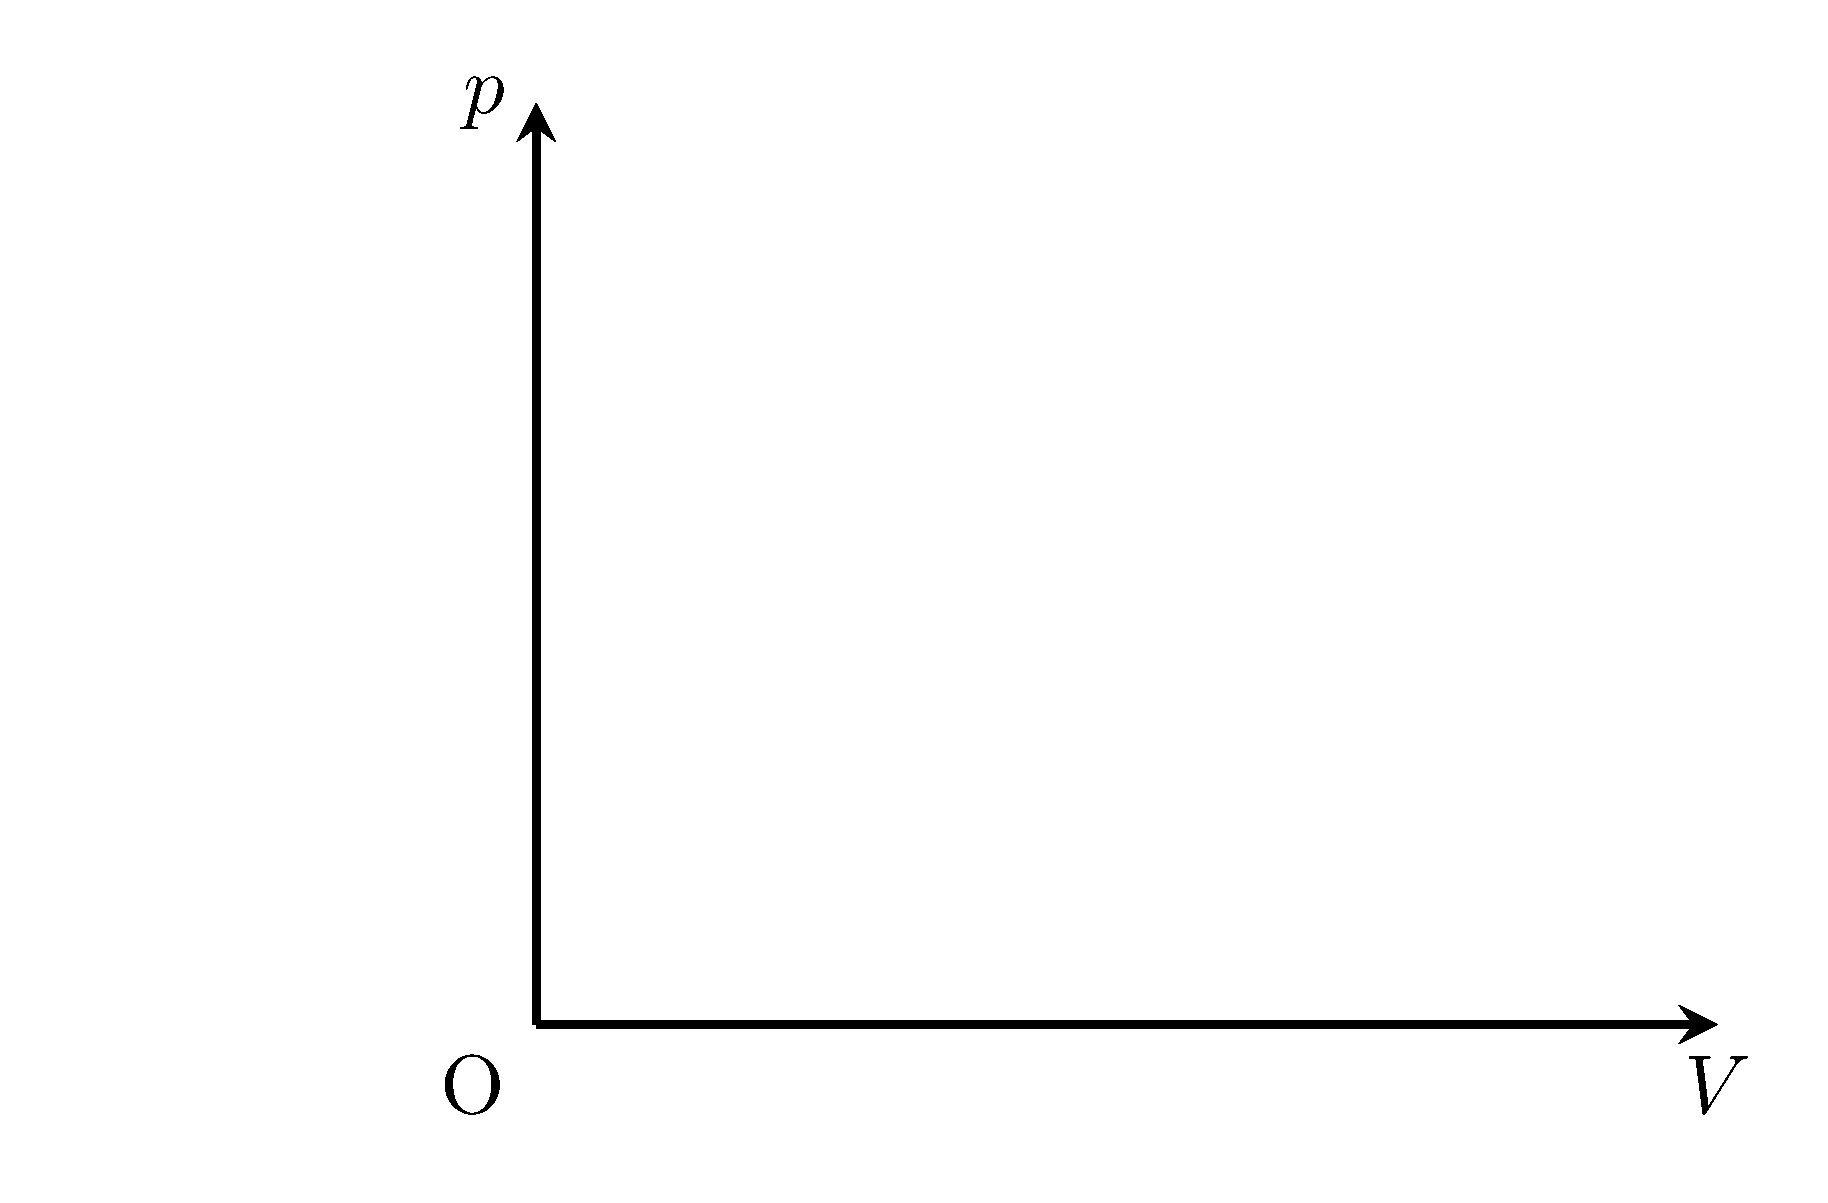
\includegraphics[keepaspectratio,width=72mm]{fig/ch16_ex9_pv_blank.png}
       \else
       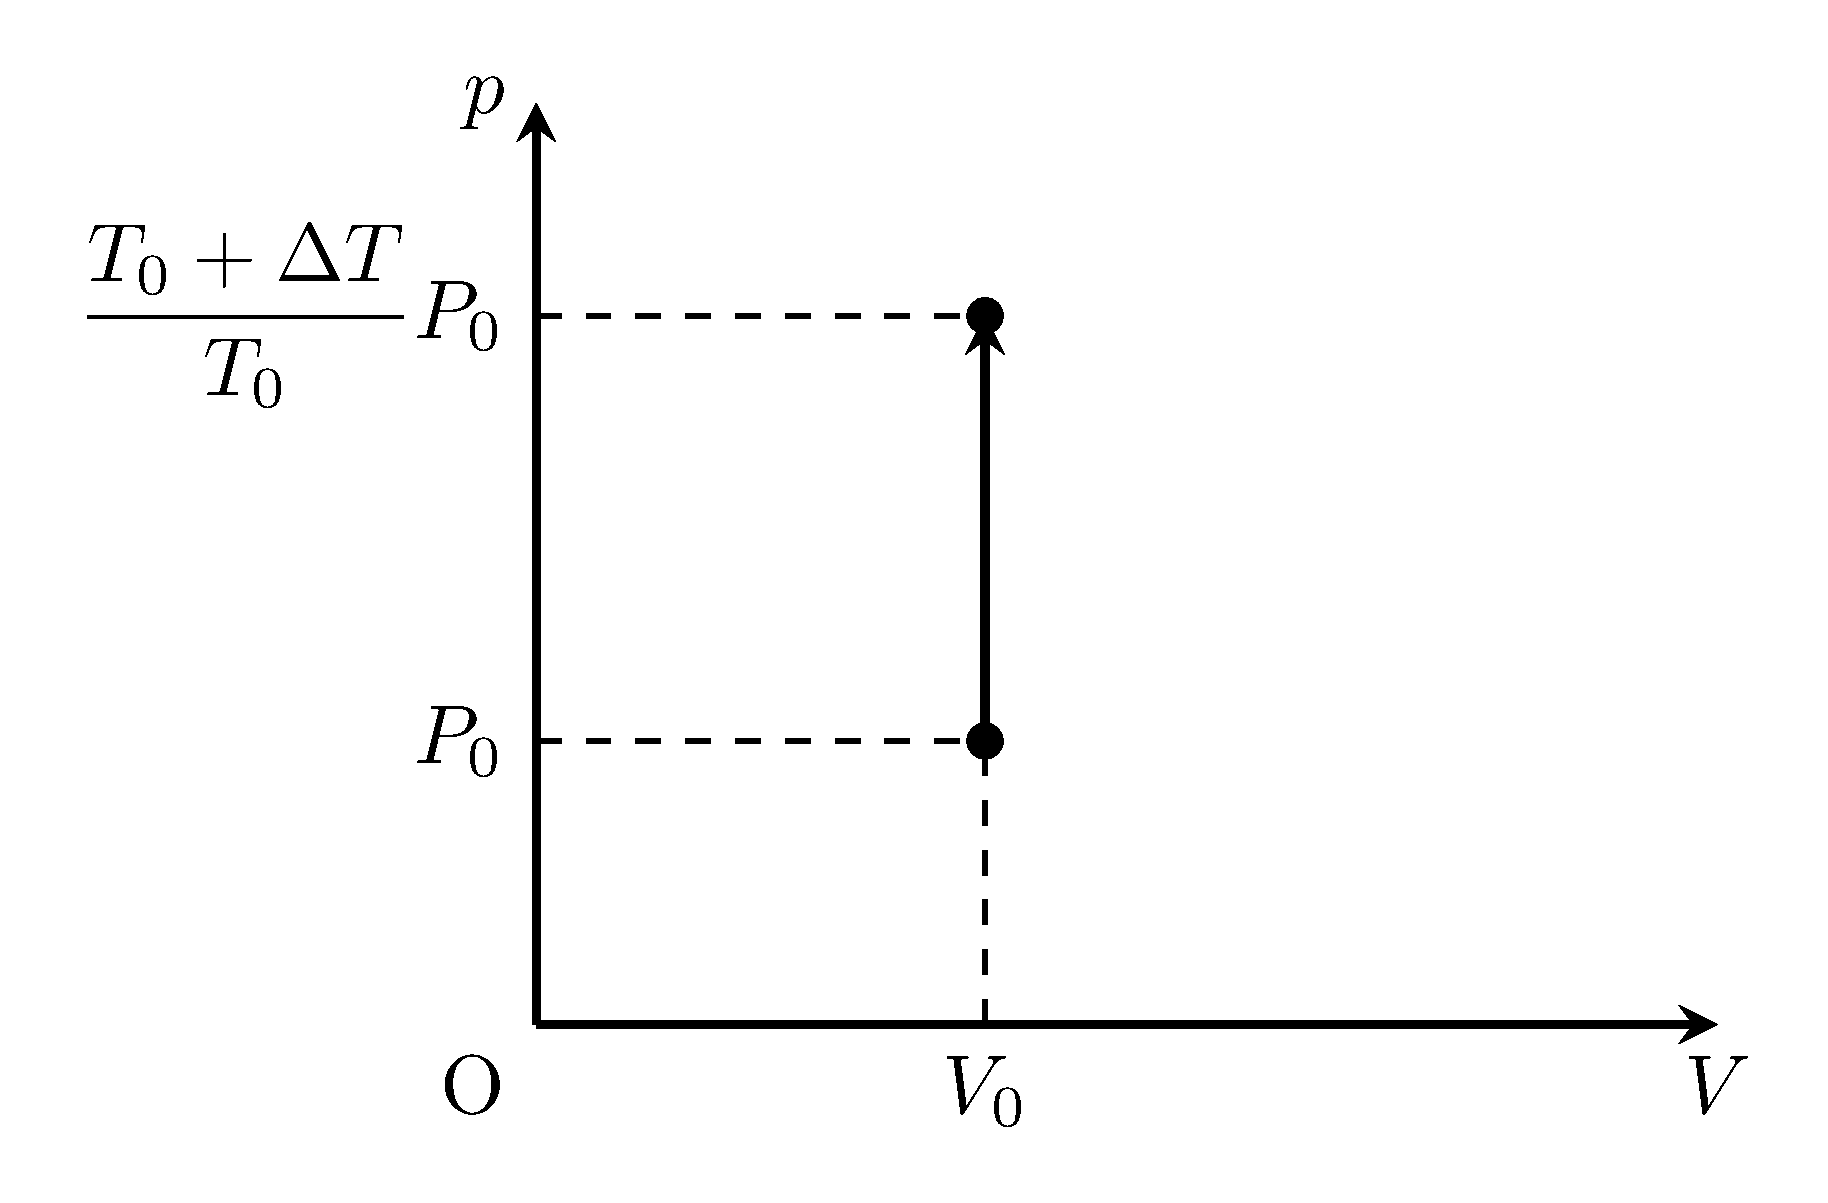
\includegraphics[keepaspectratio,width=72mm]{fig/ch16_ex9_pv.png}
       \fi
       \end{center}
       \hspace*{\fill}\Ans
\ko{2} 体積変化がないので，(1)の$P$-$V$図と$V$軸が囲む面積は0である．よって気体は外界に対して仕事をせず，
       \[w=0\U{J}\Ans\]
\ko{3} 内部エネルギーの変化は状態変化の種類によらず$\Delta U=nC_V\Delta T$と書けるので，
       \[\Delta U=nC_V\Delta T\U{J}\Ans\]
       また，熱力学第一法則$Q_{\mathrm{in}}=\Delta U+W_{\mathrm{out}}$に$Q_{\mathrm{in}}=Q$，$W_{\mathrm{out}}=w=0$を代入して，
       \AnaBD{Q=\Delta U+w=nC_V\Delta T\U{J}\Ans}
\end{komon}
\end{kaitou}
\end{reidaiunit}

%%%%%%%%%%  例題9（例題8 の直後。原本の【例題10】）  %%%%%%%%%%%%%%%%%%%%
% 再編案では原本の例題10〈定圧変化〉は落とすことになっていたが，
%   ・例題8（定積変化）と完全に対になっており，
%   ・(7)がマイヤーの関係式 C_P-C_V=R の導出そのもので，22.4・22.5 の内容と一致する
%   ・「例題はなるべく削除しない」（2026-09-03 ユーザー決定）
% ことから第22回に収めた。これで熱力学の原本例題14題を1題も落とさずに済む
%   （新21＝1〜4／新22＝5・6・7・9・10／新23＝8・11・12・13・14）。
\bsNeed{88mm}
\begin{reidaiunit}
\begin{reidai}{定圧変化（マイヤーの関係式）}
\begin{zuright}{52mm}
\hspace{1zw}図のように一様な断面積を持つシリンダーに定積モル比熱が$C_V\U{J/mol\cdot K}$の理想気体を$n\U{mol}$封入した．ピストンは軽くて自由に動くことができ，大気圧$P_0\U{Pa}$とシリンダー内の気体の圧力とが常につり合いを保つ．最初，この気体の温度は$T_0\U{K}$であった．
\zusep
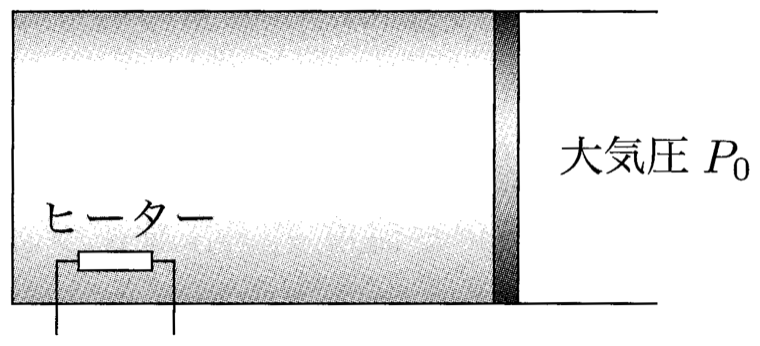
\includegraphics[keepaspectratio,width=52mm]{fig/ch16_ex10_cyl.png}
\end{zuright}
\hspace{1zw}シリンダー内にはヒーターが取り付けてあり，気体に対して熱を与えることができる．シリンダーおよびピストンは断熱材で出来ており，ヒーターによって与えた熱が大気に拡散することはないものとする．気体定数を$R\U{J/mol\cdot K}$として以下の問に答えよ．
\begin{komon}
\ko{1} 初めの状態における気体の体積$V_0\U{m^3}$を求めよ．
\end{komon}
\hspace{1zw}この状態から気体に熱をゆっくりと与え，気体の温度が$\Delta T\U{K}$だけ上昇したところで加熱を止めた．
\begin{komon}
\ko{2} この変化における気体の内部エネルギーの増加$\Delta U\U{J}$を求めよ．
\ko{3} この変化における気体の体積増加$\Delta V\U{m^3}$を求めよ．
\ko{4} この状態変化を$P$-$V$図で表せ．
\ko{5} この変化において気体が外界に対してした仕事$w\U{J}$を求めよ．
\ko{6} ヒーターによって加えた熱量$Q\U{J}$を求めよ．
\ko{7} (6)より，定積モル比熱$C_V\U{J/mol\cdot K}$と定圧モル比熱$C_P\U{J/mol\cdot K}$との間にマイヤーの関係式$C_P-C_V=R$が成立していることを示せ．
\end{komon}
\end{reidai}

\begin{sisinE}
ピストンが軽くて自由に動くので，ピストンにはたらく力のつり合い$PS=P_0S$より気体の圧力は常に大気圧$P_0$に等しい．すなわち定圧変化である．

(5) 定圧変化では$P$-$V$図が水平な線分になるので，$V$軸との間の面積は縦$P_0$・横$\Delta V$の長方形であり，$w=P_0\Delta V$と計算できる．
\end{sisinE}

\Key{状態方程式 $PV=nRT$\quad $\Delta U=nC_V\Delta T$\quad 定圧なら$W_{\mathrm{out}}=P\Delta V$\quad $Q_{\mathrm{in}}=\Delta U+W_{\mathrm{out}}$}

\begin{kaitou}
\begin{komon}
\ko{1} 初めの状態の状態方程式$P_0V_0=nRT_0$より，
       \[V_0=\frac{nRT_0}{P_0}\U{m^3}\Ans\]
\ko{2} 内部エネルギーの変化は状態変化の種類によらず，
       \[\Delta U=nC_V\Delta T\U{J}\Ans\]
\ko{3} 終状態の状態方程式は$P_0(V_0+\Delta V)=nR(T_0+\Delta T)$である．これと(1)の状態方程式の差をとって，
       \[P_0\Delta V=nR\Delta T\]
       よって，
       \[\Delta V=\frac{nR\Delta T}{P_0}\U{m^3}\Ans\]
\ko{4} 圧力が$P_0$のまま一定で，体積が$V_0$から$V_0+\Delta V$へ増加するので，$P$-$V$図は次図．
       \begin{center}
       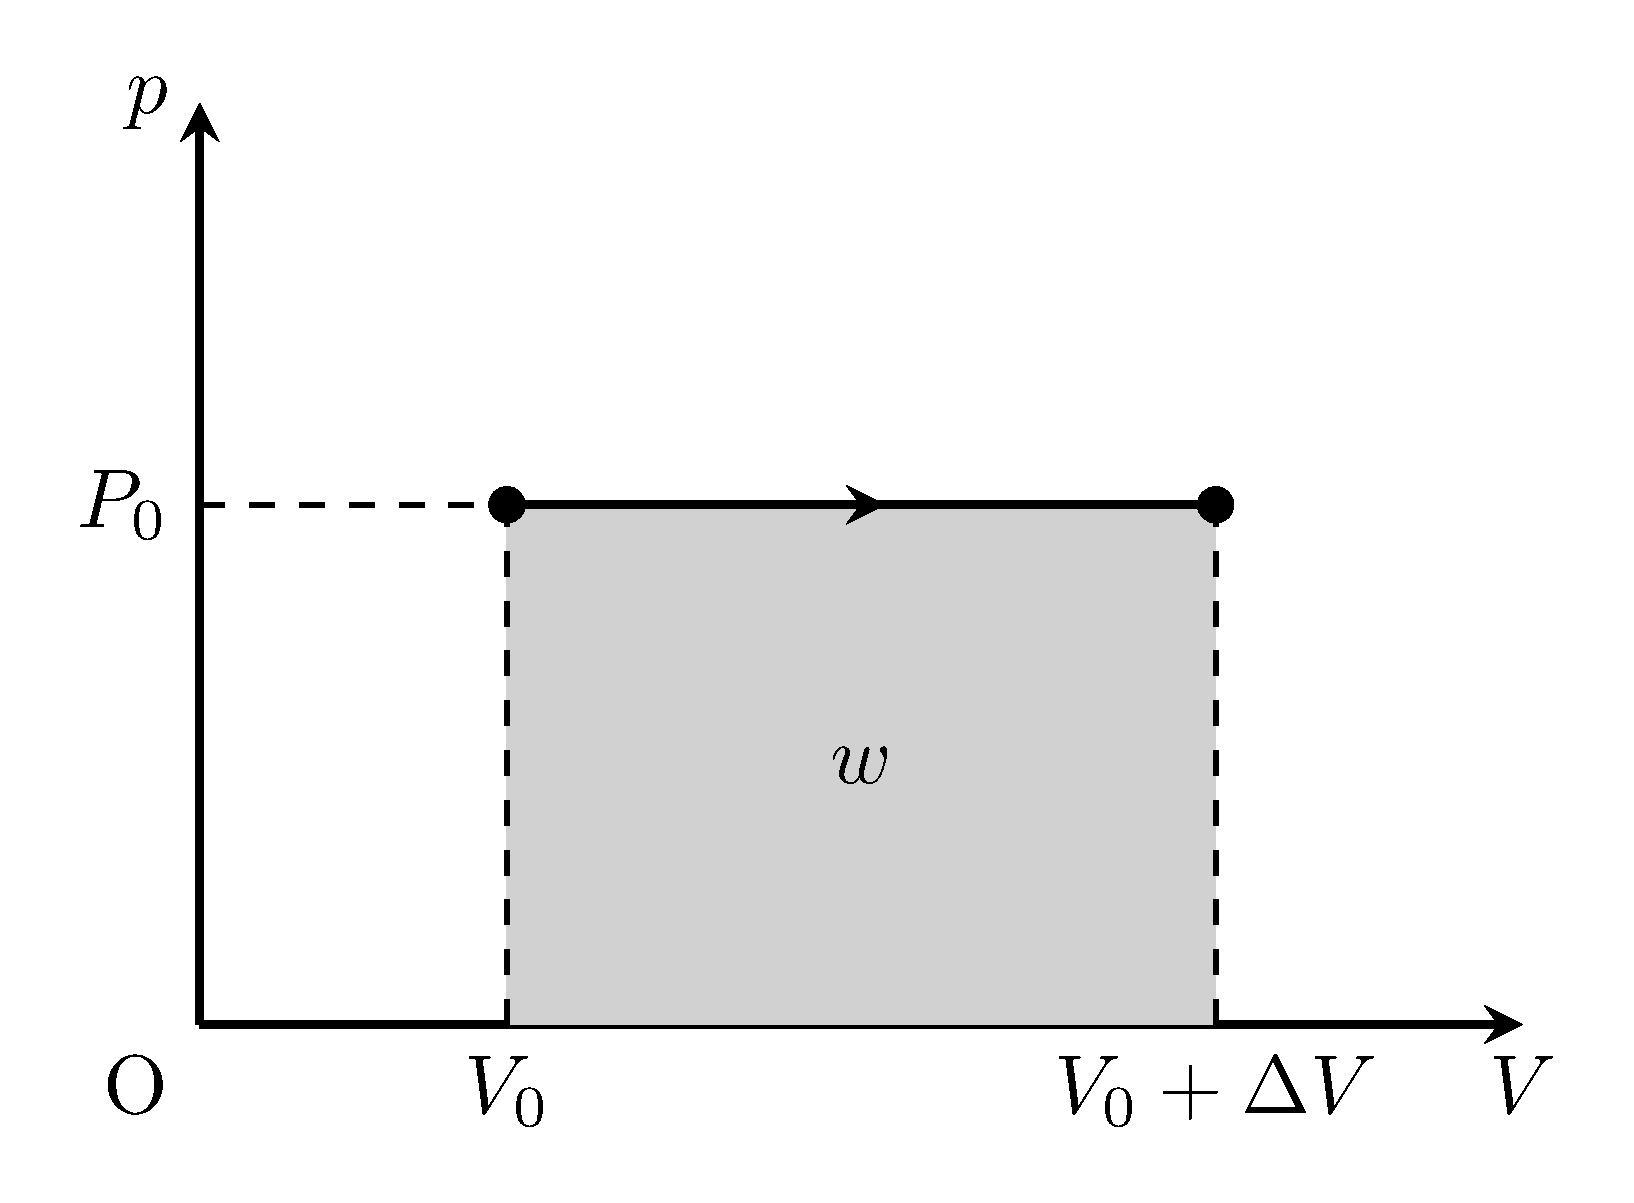
\includegraphics[keepaspectratio,width=72mm]{fig/ch16_ex10_pv.png}
       \end{center}
       \hspace*{\fill}\Ans
\ko{5} 定圧変化であるから，(4)の$P$-$V$図と$V$軸が囲む長方形の面積を求めて，
       \[w=P_0\Delta V=nR\Delta T\U{J}\Ans\]
\ko{6} 熱力学第一法則$Q_{\mathrm{in}}=\Delta U+W_{\mathrm{out}}$に(2)(5)を代入して，
       \Ana{Q=\Delta U+w=n(C_V+R)\Delta T\U{J}\Ans}
\ko{7} この状態変化は定圧変化であるから，定圧モル比熱の定義より$Q=nC_P\Delta T$とも書ける．これと(6)を比べて，
       \[nC_P\Delta T=n(C_V+R)\Delta T\]
       $\Delta T\neq 0$であるから両辺を$n\Delta T$で割って$C_P=C_V+R$，すなわち
       \[C_P-C_V=R\]
       が成立する．
\end{komon}
\end{kaitou}
\end{reidaiunit}

\newpage

%%%%%%%%%%%%%%%%%%%%  練習問題  %%%%%%%%%%%%%%%%%%%%
% 第21回の［10］に続く．章単体で組んだときも番号が本体と一致するように明示しておく
%   （make_new.sh が出す推定値より後に実行されるので，こちらが必ず勝つ）
\setcounter{qno}{10}

\filbreak
\Rank{A問題}

\Mon{基本事項の確認}

\hspace{1zw}以下の設問に答えよ．ただし気体は理想気体であるとし，気体定数を$R=8.31\U{J/mol\cdot K}$，アボガドロ数を$N_{\mathrm{A}}=6.02\times 10^{23}$\,[個/mol]とする．
\begin{komon}
\ko{1} ボルツマン定数$k_{\mathrm{B}}$はいくらか．
\ko{2} $27\Cel$における酸素分子の二乗平均速度は何$\U{m/s}$か．
\ko{3} $27\Cel$におけるヘリウム気体の1分子あたりの平均運動エネルギーは何$\U{J}$か．
\ko{4} $0.20\U{mol}$の単原子分子理想気体の温度が$10\U{K}$上昇するとき，気体の内部エネルギーの増加量は何$\U{J}$か．
\end{komon}

\filbreak
\Rank{B問題}

\Mon[\Sitei]{気体分子運動論}

% zuright の左が図より短いと差がまるごと空白になる（組版チェックリスト §3.10）ので，
%   第2段落の前半までを zuright の中に入れて図の高さに合わせた．
\begin{zuright}{40mm}
\hspace{1zw}一辺の長さが$l\U{m}$の立方体の容器の中に，分子一個の質量が$m\U{kg}$の気体分子が$N$個入っている．右図のように$x$, $y$, $z$軸をとり，分子は互いに衝突することなく，壁と気体分子は完全弾性衝突をするものとして以下の空欄に適当な式を入れよ．必要であれば単位をつけて答えよ．\par
\hspace{1zw}今ある一つの分子に着目する．この分子の速さを$v\U{m/s}$，速度成分をそれぞれ$v_x\U{m/s}$, $v_y\U{m/s}$, $v_z\U{m/s}$とすれば，この分子が壁$\mathrm{A}$に衝突してはね返される際，壁$\mathrm{A}$が分子から受ける力積の大きさは，\fbox{\MARU{1}}である．
\zusep
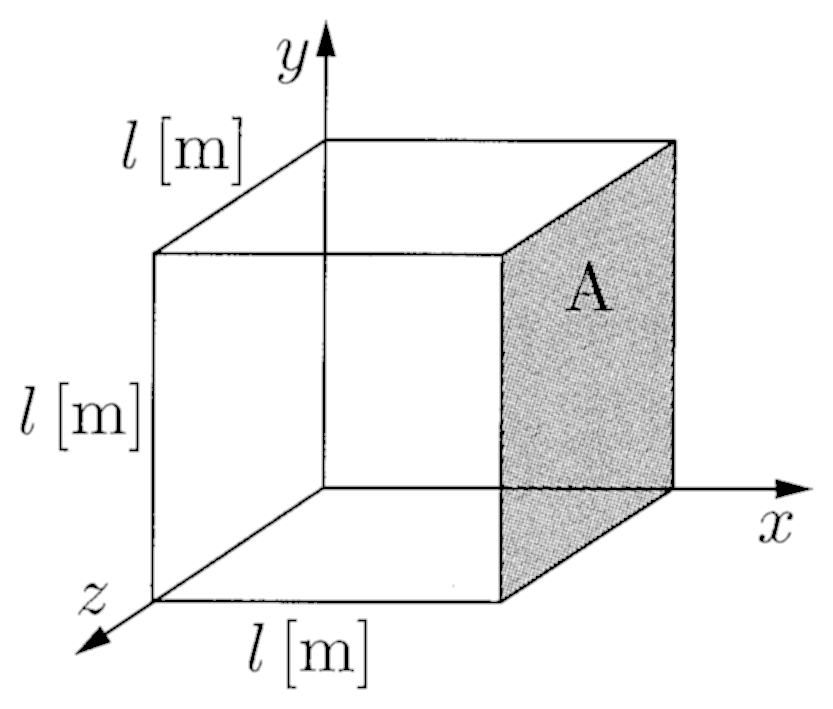
\includegraphics[keepaspectratio,width=38mm]{fig/ch15_p37_cube.png}
\end{zuright}

\noindent よって$t\U{s}$間に壁$\mathrm{A}$がこの分子から受ける力積の大きさは，\fbox{\MARU{2}}となる．
% 誤植訂正（2026-08-31，旧 physics_ch15.tex から引き継ぎ）：原本は「よってこの分子が t[s] 間に
%   壁 A がこの分子から受ける力積の大きさは」と主語が二重になっていた．
ここで$N$個の分子の速さの2乗の平均値を$\overline{v^2}$，各成分の二乗の平均値をそれぞれ$\overline{v_x^2}$, $\overline{v_y^2}$, $\overline{v_z^2}$とすると，全分子が$t\U{s}$間に壁$\mathrm{A}$に及ぼす力積$I\U{N\cdot s}$は$\overline{v_x^2}$を用いて，$I=$\fbox{\MARU{3}}となる．ここで気体分子運動の等方向性および三平方の定理を利用すると，$\overline{v^2}$と$\overline{v_x^2}$の間には\fbox{\MARU{4}}の関係が成り立つから，$\overline{v^2}$を用いて$I=$\fbox{\MARU{5}}と表せる．よって壁$\mathrm{A}$が全分子から受ける力は\fbox{\MARU{6}}$\U{N}$となるから，壁$\mathrm{A}$が受ける圧力，すなわち気体の圧力$p\U{Pa}$は，$p=$\fbox{\MARU{7}}となる．したがって，容器の体積を$V\ (=l^3)\U{m^3}$とすれば，$pV=$\fbox{\MARU{8}}となる．

\Mon{気体分子運動論}

\hspace{1zw}体積$V\U{m^3}$の容器の中に，質量$m\U{kg}$の理想気体の気体分子が$N$個入っており，容器内の気体の圧力，温度はそれぞれ$p\U{Pa}$, $T\U{K}$である．気体定数を$R\U{J/mol\cdot K}$，アボガドロ定数を$N_{\mathrm{A}}\U{/mol}$とし，前問で導出したベルヌーイの式：$pV=\dfrac{Nm\overline{v^2}}{3}$を利用して以下の設問に答えよ．
\begin{komon}
\ko{1} この気体分子の二乗平均平方根速度$\sqrt{\overline{v^2}}$を，気体の温度$T$，気体定数$R$および$1\U{mol}$あたりの気体分子の質量$M\U{kg/mol}$を用いて表せ．
\ko{2} この気体分子の二乗平均平方根速度$\sqrt{\overline{v^2}}$を，圧力$p$と密度$\rho\U{kg/m^3}$を用いて表せ．
\ko{3} この気体分子1分子あたりの平均運動エネルギー$\overline{E}\U{J}$を，温度$T$とボルツマン定数$k_{\mathrm{B}}\U{J/K}$を用いて表せ．
\end{komon}

\Mon{気体分子運動論の利用}

\hspace{1zw}気体分子の運動に関する下の各問に答えよ．ただし，気体はすべて理想気体とみなしてよい．
\begin{komon}
\ko{1} 窒素ガスの分子量を28，アボガドロ定数を$6.0\times 10^{23}\U{/mol}$，気体定数を$8.3\U{J/mol\cdot K}$とする．$300\U{K}$における窒素分子の二乗平均速度を求めよ．
\ko{2} ヘリウムガス（原子量4），ネオンガス（原子量20）について，二つのガスが同じ温度のとき，1分子あたりの平均運動エネルギーの比を求めよ．
\ko{3} ヘリウムガスについて，温度が$273\Cel$になったときのヘリウム1分子あたりの平均運動エネルギーおよび二乗平均速度は$0\Cel$の時のそれぞれ何倍となるか．
\end{komon}

\Mon[\Sitei]{内部エネルギー}

\hspace{1zw}温度が$T\U{K}$の単原子分子理想気体が$n\U{mol}$ある．気体定数を$R\U{J/mol\cdot K}$として以下の設問に答えよ．
\begin{komon}
\ko{1} 温度を一定に保って体積を$m$倍にするとき，内部エネルギーは何倍になるか．
\ko{2} 圧力を一定に保って体積を$m$倍にするとき，内部エネルギーは何倍になるか．
\end{komon}

\begin{zuright}{38mm}
\hspace{1zw}温度が$T\U{K}$のこの気体を図のような断熱材で出来た体積$V\U{m^3}$の箱に圧力が$P\U{Pa}$となるまで封入し，ヒーターを用いて$Q\U{J}$の熱を気体に与えたところ，気体の温度は$T'\U{K}$となった．この状態変化では気体の体積が変わらないため，気体は仕事のやり取りをしない．このことを利用して，以下の設問に答えよ．
\begin{komon}
\ko{3} 熱力学第一法則を用いて，気体の上昇温度$\Delta T=T'-T$を求めよ．
\ko{4} 気体の圧力$P'$を求めよ．
\end{komon}
\zusep
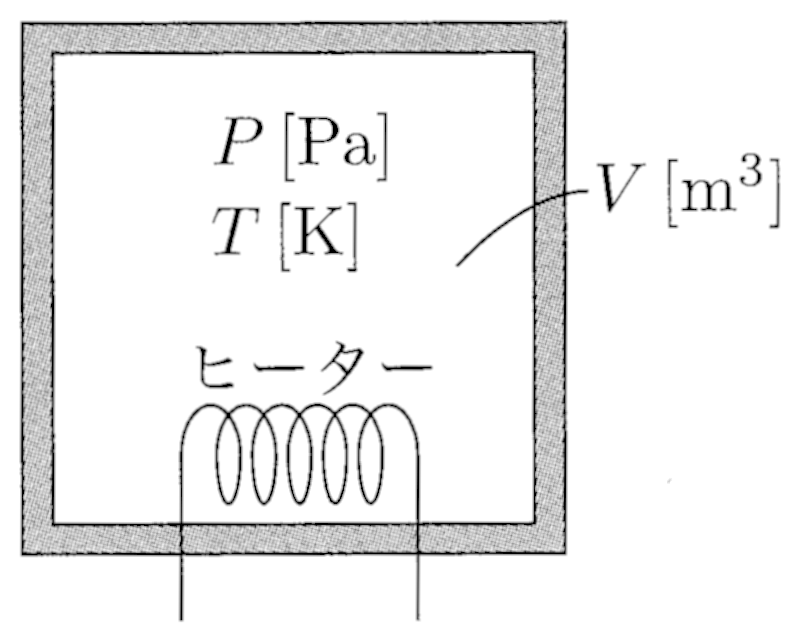
\includegraphics[keepaspectratio,width=38mm]{fig/ch15_p38_box.png}
\end{zuright}

\Mon{$p$-$V$図}

\begin{zuright}{40mm}
\hspace{1zw}一定量の理想気体の状態を右図の矢印の順に静かに変化させた．$\mathrm{A}$での圧力が$2p_0\U{Pa}$であるときについて，この状態変化を$p$-$V$図上での変化に書き直せ．ただし，グラフには$\mathrm{A}$, $\mathrm{B}$, $\mathrm{C}$点を明示し，変化の方向に矢印をつけること．
\zusep
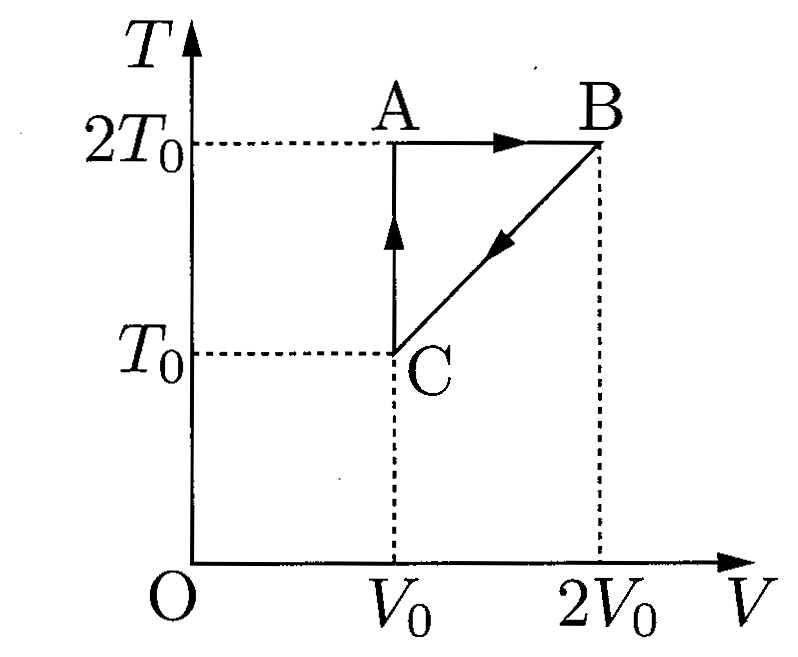
\includegraphics[keepaspectratio,width=40mm]{fig/ch15_p38_tv.png}
\end{zuright}

\Mon{定圧変化}

\begin{zuright}{58mm}
\hspace{1zw}右図のように断面積$S\U{m^2}$のシリンダーの中に，なめらかに動くことのできるピストンを用いて定積モル比熱が$C_V\U{J/mol\cdot K}$の理想気体を$n\U{mol}$だけ封入した．ピストンは軽くて自由に動くことができ，ピストンの右側は大気に通じている．初め，シリンダーの底からピストンまでの距離は$l_0\U{m}$であり，また気体の温度は$T_0\U{K}$であった．
\zusep
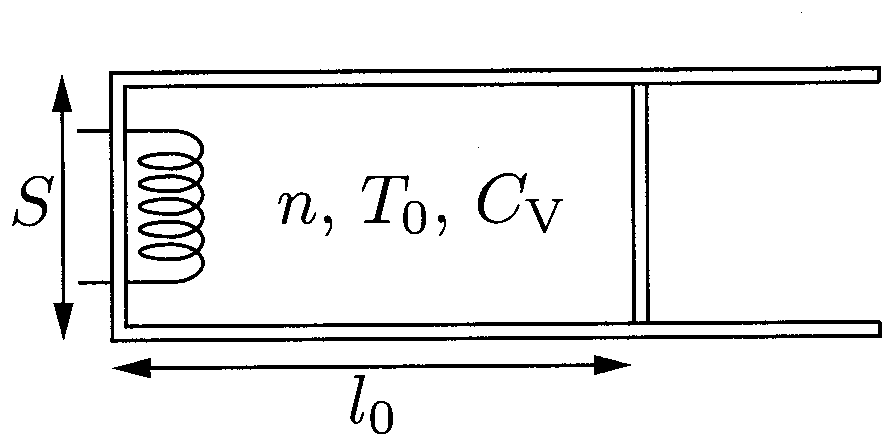
\includegraphics[keepaspectratio,width=58mm]{fig/ch16_p40_cyl.png}
\end{zuright}
\hspace{1zw}シリンダー内にはヒーターが取り付けられており，気体に対して熱を与えることができる．シリンダーおよびピストンは断熱材でできており，ヒーターによって与えた熱が大気に拡散することはないものとする．気体定数を$R\U{J/mol\cdot K}$として以下の設問に答えよ．
\begin{komon}
\ko{1} 大気圧$p_0\U{Pa}$を求めよ．
\end{komon}
\hspace{1zw}この状態から内部の気体をヒーターで少しずつ熱したところ，ピストンはゆっくりと移動し，シリンダーの底からピストンまでの距離は$l_1\U{m}$となった．
\begin{komon}
\ko{2} 終状態における気体の温度$T_1\U{K}$を求めよ．
\ko{3} この状態変化を$p$-$V$図で表せ．
\ko{4} この変化において，気体が外界にした仕事$w\U{J}$を求めよ．
\ko{5} ヒーターによって加えた熱量$Q\U{J}$を求めよ．
\end{komon}

\Mon{定積変化}

\begin{zuright}{58mm}
\hspace{1zw}右図のように断面積$S\U{m^2}$のシリンダーの中に定積モル比熱が$C_V\U{J/mol\cdot K}$の理想気体を$n\U{mol}$だけ封入し，ピストンの位置を固定して動かないようにした．このときのシリンダーの底からピストンまでの距離は$l_0\U{m}$であり，また気体の温度は$T_0\U{K}$であった．
\zusep
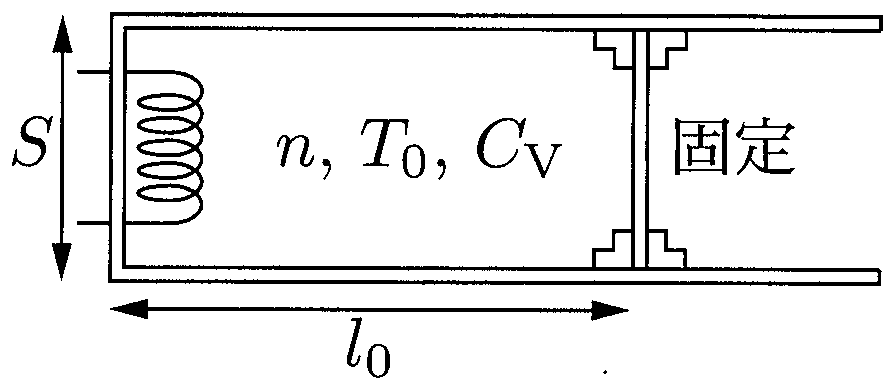
\includegraphics[keepaspectratio,width=58mm]{fig/ch16_p41_cyl.png}
\end{zuright}
\hspace{1zw}シリンダー内にはヒーターが取り付けられており，気体に対して熱を与えることができる．シリンダーおよびピストンは断熱材でできており，ヒーターによって与えた熱が大気に拡散することはないものとする．この状態からゆっくり熱し，内部の気体の温度が$T_1\U{K}$になったところで加熱を止めた．気体定数を$R\U{J/mol\cdot K}$として以下の設問に答えよ．
\begin{komon}
\ko{1} 初状態および終状態における気体の圧力$p_0\U{Pa}$, $p_1\U{Pa}$を求めよ．
\ko{2} この状態変化を$p$-$V$図で表せ．
\ko{3} この変化において，気体が外界にした仕事$w\U{J}$を求めよ．
\ko{4} ヒーターによって加えた熱量$Q\U{J}$を求めよ．
\end{komon}

\filbreak
\Rank{C問題}

\Mon{球内での気体分子運動論}

\hspace{1zw}以下の空欄に適当な式を入れよ．

\begin{zuright}{40mm}
\hspace{1zw}半径$a\U{m}$の球形の容器の中に，質量$m\U{kg}$の気体分子が$N$個入っている．簡単のために，気体の各分子は一定の速さ$v\U{m/s}$で容器内を不規則な方向に飛び交っており，分子同士は互いに衝突することなく，器壁と完全弾性衝突を繰り返しているものとして考えよう．今，ある一つの分子に着目すると，この分子は器壁と衝突を繰り返して飛び回っているが，その軌跡は必ず球の中心$\mathrm{O}$を含むある一つの面内にある．これを図示したのが右図である．
\zusep
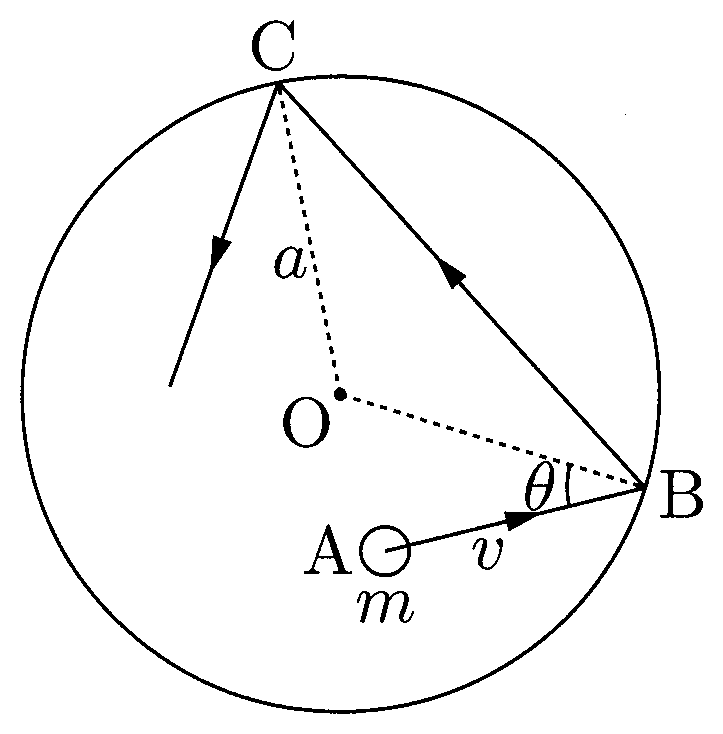
\includegraphics[keepaspectratio,width=40mm]{fig/ch15_p39_sphere.png}
\end{zuright}
% 誤植訂正（2026-08-31，旧 physics_ch15.tex から引き継ぎ）：原本は「内径 a[m] の球形の容器」
%   だが，図でも解答でも a は中心 O から器壁までの距離（半径）として使われている．

\hspace{1zw}さて，今，この分子が入射角$\theta$で器壁の一点$\mathrm{B}$に衝突したとすると，力積を及ぼしあう方向は半径$\mathrm{OB}$方向であるから，これに垂直な方向の速度成分は衝突の前後で変化しない．よって，衝突によるこの分子の運動量の変化は\fbox{\MARU{1}}方向に大きさ\fbox{\MARU{2}}$\U{N\cdot s}$である．次の衝突までの時間は\fbox{\MARU{3}}$\U{s}$であり，図から分かるように各回の衝突から衝突までの時間間隔は同じになるから，時間$t\U{s}$中の衝突回数は\fbox{\MARU{4}}回になる．したがって，この分子が時間$t\U{s}$中に壁面に対して与えた力積の大きさの総和は\fbox{\MARU{5}}$\U{N\cdot s}$である．

\hspace{1zw}さて，気体分子はそれぞれ運動方向が異なるため，壁面への入射角$\theta$は気体分子ごとに異なるが，\MARU{5}の答えは$\theta$に依存していない．すなわち，速度ベクトルの向きが異なる他の分子についても壁面に対して与える力積の大きさは同じになるので，$N$個の分子が時間$t\U{s}$間の間に器壁に与える力積の大きさは\fbox{\MARU{6}}$\U{N\cdot s}$となる．よって，器壁に対して及ぼす平均の力の大きさは\fbox{\MARU{7}}$\U{N}$となる．したがって容器内の圧力，つまり気体の圧力$p\U{Pa}$は\fbox{\MARU{8}}となり，また，容器の容積を$V\U{m^3}$とすると，$pV=$\fbox{\MARU{9}}と表せる．

\Mon{定積・定圧変化}

\begin{zuright}{34mm}
\hspace{1zw}右図のように鉛直に立ててある断面積$S\U{m^2}$のシリンダーの中に，質量$M\U{kg}$のなめらかに動くことのできるピストンで，定積モル比熱が$C_V\U{J/mol\cdot K}$の理想気体を$n\U{mol}$だけ封入した．初め，ピストンはシリンダーの底から$l_0\U{m}$の高さのところにあるストッパーにのっており，大気の圧力は$P_0\U{Pa}$，シリンダー内の気体の温度は$T_0\U{K}$であった．シリンダー内にはヒーターが取り付けられており，気体に対して熱を与えることができる．シリンダーおよびピストンは断熱材で出来ており，ヒーターによって与えた熱が大気に拡散することはないものとする．気体定数を$R\U{J/mol\cdot K}$，重力加速度の大きさを$g\U{m/s^2}$として以下の設問に答えよ．
\zusep
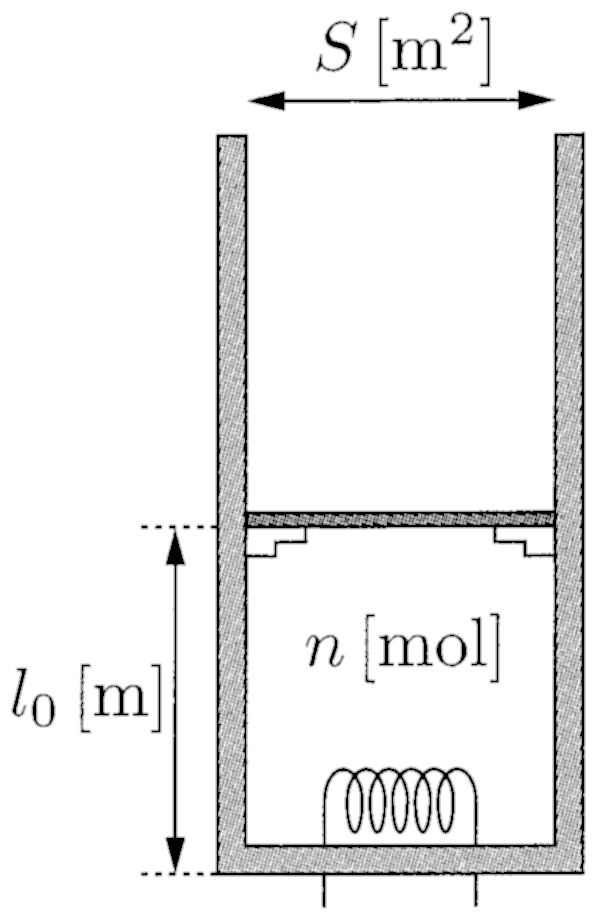
\includegraphics[keepaspectratio,width=30mm]{fig/ch16_p42_vcyl.png}
\end{zuright}
\begin{komon}
\ko{1} 初めの状態におけるシリンダー内の気体の圧力$p'\U{Pa}$を求めよ．
\end{komon}
\hspace{1zw}この状態から内部の気体をヒーターで少しずつ熱したところ，ピストンは静止したままであったが，しばらくすると動き始めた．さらに加熱を続けると，ピストンはゆっくりと上昇し，シリンダーの底からピストンまでの距離は$l_1\U{m}$となった．
\begin{komon}
\ko{2} ピストンが動き始めたときのシリンダー内の気体の温度$T_1\U{K}$を求めよ．
\ko{3} 終状態における気体の温度$T_2\U{K}$を求めよ．
\ko{4} ピストンが動き始める前と後とに分けて考えることに注意して，最初の状態からこの状態に至るまでの間にヒーターによって気体に与えられた総熱量$Q\U{J}$を求めよ．
\end{komon}

\Mon[\Sitei]{断熱変化における気体分子運動論}

% 原本の 第18回（熱力学総合演習）章末[34]．`physics_ch18.tex` はページ画像の貼り込みの
%   ままだったので，問題編 prob_p47.png（問題・図）から新規に起こした．
%   装置図は texify_draft/mkfig_new22.py で再生成できる（fig/n22_a21_cyl.png）．
\begin{zuright}{46mm}
\hspace{1zw}右図のように断熱材でできた，断面積$S\U{m^2}$，長さ$l\U{m}$のシリンダーとピストンからなる，容積$Sl\U{m^3}$の容器に温度$T\U{K}$の気体が封入されている．気体は質量$m\U{kg}$の単原子分子$N$個からなり，分子と容器の壁との衝突は完全弾性衝突であるとして，以下の空欄に適当な式を入れよ．必要なものには単位をつけて答えよ．
\zusep
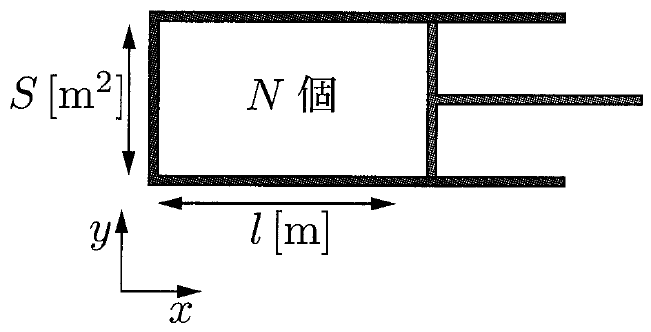
\includegraphics[keepaspectratio,width=46mm]{fig/n22_a21_cyl.png}
\end{zuright}

\hspace{1zw}ピストンの面に垂直な方向に$x$軸をとる．今一つの分子に着目し，$x$軸方向の速さを$v_x\U{m/s}$とすると，この分子がピストンと衝突するたびに，分子はピストンに大きさ\fbox{\MARU{1}}の力積を与える．この衝突は$1\U{s}$あたり\fbox{\MARU{2}}回起こるので，この分子が$1\U{s}$あたりにピストンに及ぼす力積の大きさは\fbox{\MARU{3}}である．よって全分子について$v_x^2$の平均をとりその平均値を$\overline{v_x^2}$とすれば，ピストンが受ける圧力$p\U{Pa}$は，$p=$\fbox{\MARU{4}}となる．ここで，理想気体の状態方程式$pV=Nk_{\mathrm{B}}T$を利用すると，$\overline{v_x^2}$と$T$の間の関係は，\fbox{\MARU{5}}と求められる．

\hspace{1zw}さて，ピストンを一定の速さ$u\U{m/s}$で容器の容積を小さくする方向に移動させたとする．このピストンに$x$方向の速さ$v_x\U{m/s}$をもった分子が衝突すると，衝突後の$x$方向の速さは\fbox{\MARU{6}}となる．$u$は$v_x$に比べて十分小さいとして$u$の2次以上の項を無視すると，$x$方向の速さの二乗は一回の衝突によって\fbox{\MARU{7}}だけ増加する．ここで，ピストンが微小距離$\Delta l\U{m}$$(\ll l)$だけ動く微小時間について考える．微小時間について考えているので，$u\ll v_x$であるからピストンが移動している最中の分子の速さの変化は$v_x$に比べて十分小さく，またその気体分子の運動の往復距離もほとんど$2l\U{m}$のままとみなしてよいことに注意すると，ピストンが移動する間にこの分子がピストンに衝突する回数は近似的に\fbox{\MARU{8}}回とみなせる．よって，この間に$x$方向の速さの二乗は\fbox{\MARU{9}}だけ増加する．これにより，気体分子の$x$軸方向の運動エネルギー$\dfrac{1}{2}mv_x^2$が増加するが，この増加は，気体分子運動の等方向性より，分子間の衝突によって$x, y, z$方向の速さの二乗の平均値が等しくなるように（すなわち各軸方向の運動エネルギーが等しくなるように）分配されるから，結局，$x$方向の速さの二乗の平均値は\fbox{\MARU{10}}だけしか増加しない．
% 誤植訂正（2026-09-20）：原本は「各軸方向の運動エネルギーが久しくなるように」．「等しく」の誤植．
ここで\MARU{5}の関係を用いると，温度は$T, l, \Delta l$を用いて\fbox{\MARU{11}}だけ増加することになり，この操作による気体の体積の変化$\Delta V\ (=-S\Delta l)\U{m^3}$および気体の体積$V\ (=Sl)\U{m^3}$を用いると，気体の温度は$\Delta T=-\dfrac{2T}{3V}\Delta V\U{K}$だけ上昇する．これが気体の断熱圧縮による温度上昇である．

\newpage

%%%%%%%%%%%%%%%%%%%%  解答  %%%%%%%%%%%%%%%%%%%%
\KaiTitle{第22回　気体分子運動論と内部エネルギー}
\setlength{\columnseprule}{0.4pt}
\begin{multicols}{2}
\raggedcolumns

\Rank{A問題}
\MonN{11}{基本事項の確認}\par\nopagebreak
\begin{sisin}
ボルツマン定数の定義式をよく覚えておこう．また，気体の内部エネルギーの式$U=\dfrac{3}{2}nRT$は単原子分子理想気体に対してしか成立しないが，気体分子の二乗平均速度$\sqrt{\overline{v^2}}=\sqrt{\dfrac{3RT}{M}}$は理想気体でさえあれば成立し，二原子分子などに対しても利用できる式である．二乗平均速度の公式を利用する際には，分子量を$\U{kg/mol}$の単位にしてから$M$に代入することを忘れないようにせよ．
\end{sisin}
\KaiHead
\begin{komon}
\ko{1} ボルツマン定数は気体1分子あたりの気体定数といえるので，
       \[k_{\mathrm{B}}=\frac{R}{N_{\mathrm{A}}}=\frac{8.31}{6.02\times 10^{23}}\]
       \hspace*{2zw}$\fallingdotseq 1.38\times 10^{-23}\U{J/K}$\Ans
\ko{2} 酸素分子$\mathrm{O_2}$の分子量は$32\U{g/mol}$であるから，$M=32\times 10^{-3}\U{kg/mol}$である．よって，
       \[\sqrt{\overline{v^2}}=\sqrt{\frac{3RT}{M}}=\sqrt{\frac{3\cdot 8.31\cdot 300}{32\times 10^{-3}}}\]
       \hspace*{2zw}$\fallingdotseq 4.83\times 10^2\U{m/s}$\Ans
\ko{3} $1\U{mol}$あたりの内部エネルギーを考えると，ヘリウムは単原子分子であるから，
       \[U=\frac{3}{2}\times 1\cdot R\cdot 300\U{J}\]
       これはヘリウム気体分子の運動エネルギーの総和ゆえ，一分子あたりの平均運動エネルギーは，
       \[E=\frac{U}{N_{\mathrm{A}}}=\frac{3}{2}\cdot\frac{R}{N_{\mathrm{A}}}\cdot 300=\frac{3}{2}k_{\mathrm{B}}\cdot 300\]
       \hspace*{2zw}$\fallingdotseq 6.21\times 10^{-21}\U{J}$\Ans
\ko{4} $T\to T+10\U{K}$へ温度上昇するときの内部エネルギーの増加量は，(変化後)$-$(変化前)を求めて，
       \[\Delta U=\frac{3}{2}nR\cdot(T+10)-\frac{3}{2}nRT\]
       \hspace*{2zw}$=\dfrac{3}{2}\cdot 0.20\cdot 8.31\cdot 10\fallingdotseq 24.9\U{J}$\Ans
\end{komon}

\Rank{B問題}
\MonN[\Sitei]{12}{気体分子運動論}\par\nopagebreak
\begin{sisin}
気体分子運動論の問題を解く際に，ミスしやすい点を以下に挙げる．これらのキーポイントをミスしないように注意すること．
\begin{komon}
\ko{1} 分子が壁$\mathrm{A}$に与えた力積と，壁$\mathrm{A}$が分子に与えた力積とを混同してはならない．分子の運動量変化から求められるのは分子が受けた力積，すなわち壁$\mathrm{A}$が分子に与えた力積である．作用・反作用の法則より，分子が壁$\mathrm{A}$に与えた力積は，壁$\mathrm{A}$が分子に与えた力積と等大逆向きである．
\ko{2} 分子が壁$\mathrm{A}$に衝突してから再び壁$\mathrm{A}$に衝突するには，分子は容器内を\underline{往復し}\hskip0pt\underline{なけれ}\hskip0pt\underline{ばなら}\hskip0pt\underline{ない}．各分子の速度成分の大きさは弾性衝突によって変化せず，速さは一定とみなしてよいので，例えば$x$軸方向に往復分$2l$の道のりを動くのに要する時間は$\dfrac{2l}{v_x}$となる．
\ko{6} 力積と力とを混同してはならない．力積とは平均の力$\times$時間であるから，力積から力を計算するには，力積を作用していた時間で割る必要がある．
\end{komon}
\end{sisin}
\KaiHead
\begin{komon}
\ko{1} 分子と壁$\mathrm{A}$との衝突は完全弾性衝突であるから，衝突前後でこの分子の速度は$x$成分のみが$v_x$から$-v_x$へ変化する．よって衝突による分子の運動量ベクトルの変化は，
       \[\begin{aligned}
         \Delta\overrightarrow{p}&=m\begin{pmatrix}-v_x\\ v_y\\ v_z\end{pmatrix}-m\begin{pmatrix}v_x\\ v_y\\ v_z\end{pmatrix}\\[1mm]
         &=\begin{pmatrix}-2mv_x\\ 0\\ 0\end{pmatrix}
       \end{aligned}\]
       であり，これは壁$\mathrm{A}$が分子に対して与えた力積である．ここで作用・反作用の関係より，衝突の際に分子が壁$\mathrm{A}$に対して与えた力積$\overrightarrow{I_m}$は，壁$\mathrm{A}$が分子に対して与えた力積と等大逆向きになるので，
       \[\overrightarrow{I_m}=-\begin{pmatrix}-2mv_x\\ 0\\ 0\end{pmatrix}=\begin{pmatrix}2mv_x\\ 0\\ 0\end{pmatrix}\]
       である．よって，大きさは$2mv_x\U{N\cdot s}$\Ans
\ko{2} 壁$\mathrm{A}$に衝突した後，分子が$x$軸方向に往復分の$2l$の道のりを進むと，再び壁$\mathrm{A}$に衝突する．分子の$x$軸方向の速さは，衝突によらず一定値$v_x$であるから，一往復に要する時間は$\dfrac{2l}{v_x}$である．よって，この分子は$t\U{s}$間に壁$\mathrm{A}$と$\dfrac{v_xt}{2l}$回衝突する．\par
       \hspace*{1zw}以上と(1)より，$t\U{s}$間にこの分子が壁$\mathrm{A}$に対して及ぼす力積の大きさは，
       \[2mv_x\cdot\frac{v_xt}{2l}=\frac{mv_x^2t}{l}\U{N\cdot s}\Ans\]
\ko{3} 各分子ごとに速度の$x$成分の二乗値の$v_x^2$が異なるので，(2)で求めた，$t\U{s}$間に分子が壁$\mathrm{A}$に対して及ぼす力積の大きさは分子ごとに異なるが，$v_x^2$の平均値を$\overline{v_x^2}$とすると，$t\U{s}$間に壁$\mathrm{A}$に対して及ぼす力積の大きさの平均値は，一分子あたり
       \[\frac{m\overline{v_x^2}t}{l}\U{N\cdot s}\]
       である．全分子は$N$個だから，
       \[I=N\frac{m\overline{v_x^2}t}{l}\U{N\cdot s}\Ans\]
\ko{4} $v$と$v_x$, $v_y$, $v_z$の間には三平方の定理より
       \[v^2=v_x^2+v_y^2+v_z^2\]
       が成立する．全分子に対して両辺それぞれ平均を取ると，
       \[\overline{v^2}=\overline{v_x^2}+\overline{v_y^2}+\overline{v_z^2}\]
       が成立する．また気体分子運動の等方向性より，各軸方向の速度成分の二乗の平均値の間に，
       \[\overline{v_x^2}=\overline{v_y^2}=\overline{v_z^2}\]
       が成立する．以上より，
       \[\overline{v_x^2}=\frac{1}{3}\overline{v^2}\Ans\]
\ko{5} (3)(4)を用いて，
       \[I=\frac{Nm\cdot\frac{1}{3}\overline{v^2}\cdot t}{l}=\frac{Nm\overline{v^2}t}{3l}\U{N\cdot s}\Ans\]
\ko{6} 壁$\mathrm{A}$が全分子から受ける平均の力を$\overline{F}\U{N}$とすれば，平均の力の定義より，$I$, $\overline{F}$, $t$の間に
       \[I=\overline{F}\cdot t\]
       が成り立つ．よって，
       \[\overline{F}=\frac{I}{t}=\frac{Nm\overline{v^2}}{3l}\U{N}\Ans\]
\ko{7} 壁$\mathrm{A}$の面積は$l^2$であるから，気体の圧力は
       \[p=\frac{\overline{F}}{l^2}=\frac{Nm\overline{v^2}}{3l^3}\U{Pa}\Ans\]
\ko{8} (7)および$V=l^3$より，
       \[p=\frac{Nm\overline{v^2}}{3V}\]
       これより，
       \[pV=\frac{Nm\overline{v^2}}{3}\Ans\]
\end{komon}

\MonN{13}{気体分子運動論}\par\nopagebreak
\begin{sisin}
前問で得られたベルヌーイの式は，気体分子運動と気体の圧力を結びつける式である．一方，理想気体の状態方程式$pV=nRT$は気体の圧力と気体の温度とを結びつける式である．よって，この二つを組み合わせれば，気体の温度と気体の分子運動（二乗平均速度など）とを結びつけることができる．あとはこれによって得られた式を，問題条件で要求されている変数にうまく置き換えていこう．
\end{sisin}
\KaiHead
\begin{komon}
\ko{1} 気体分子運動論のベルヌーイの式より，
       \[pV=\frac{Nm\overline{v^2}}{3}\]
       である．またこの理想気体の物質量は$n=\dfrac{N}{N_{\mathrm{A}}}\U{mol}$であるから，状態方程式は，
       \[pV=\frac{N}{N_{\mathrm{A}}}RT\]
       である．以上2式の両辺を結ぶと
       \[\frac{Nm\overline{v^2}}{3}=\frac{N}{N_{\mathrm{A}}}RT\]
       であり，これを変形すると，
       \[\overline{v^2}=\frac{3RT}{mN_{\mathrm{A}}}\]
       となる．ここで，$mN_{\mathrm{A}}$は気体分子$1\U{mol}$あたりの質量$M\U{kg/mol}$を表しているので，
       \[\overline{v^2}=\frac{3RT}{M}\]
       である．以上より，
       \[\sqrt{\overline{v^2}}=\sqrt{\frac{3RT}{M}}\U{m/s}\Ans\]
\ko{2} 密度$\rho$は，単位体積当たりの質量である．気体分子の全質量は$M\cdot n\U{kg}$であるから，
       \[\rho=\frac{M\cdot n}{V}\U{kg/m^3}\]
       であるが，状態方程式$pV=nRT$より$\dfrac{p}{RT}=\dfrac{n}{V}$であるから，
       \[\rho=\frac{pM}{RT}\U{kg/m^3}\]
       と表せる．よって，$\dfrac{RT}{M}=\dfrac{p}{\rho}$であるから，(1)で得られた答を書き換えて，
       % 誤植訂正（2026-08-31）：原本は「(2)で得られた答を書き換えて」だが，
       %   書き換えているのは(1)の答なので「(1)」に改めた．
       \[\sqrt{\overline{v^2}}=\sqrt{\frac{3p}{\rho}}\U{m/s}\Ans\]
\ko{3} 気体分子の平均運動エネルギー$\overline{E}$は，
       \[\begin{aligned}
         \overline{E}&=\frac{1}{2}m\overline{v^2}=\frac{1}{2}m\cdot\frac{3RT}{M}=\frac{1}{2}m\cdot\frac{3RT}{mN_{\mathrm{A}}}\\[1mm]
         &=\frac{3RT}{2N_{\mathrm{A}}}
       \end{aligned}\]
       と表せる．
       \[k_{\mathrm{B}}=\frac{R}{N_{\mathrm{A}}}\]
       を用いて$\overline{E}$を書き換えると，
       \[\overline{E}=\frac{3}{2}k_{\mathrm{B}}T\U{J}\Ans\]
\end{komon}
\begin{chuu}
A問題においては，ヘリウム一分子が持つ運動エネルギーを，気体の内部エネルギー$U=\dfrac{3}{2}nRT$を気体の分子数で割り算することによって求めたが，\underline{この方}\hskip0pt\underline{法は単}\hskip0pt\underline{原子分}\hskip0pt\underline{子理想}\hskip0pt\underline{気体で}\hskip0pt\underline{なけれ}\hskip0pt\underline{ば利用}\hskip0pt\underline{するこ}\hskip0pt\underline{とがで}\hskip0pt\underline{きない}．なぜなら，気体の内部エネルギーの結果式$U=\dfrac{3}{2}nRT$は単原子分子理想気体でなければ成立しないからである．ところが，本問で導いた気体分子一分子あたりの平均運動エネルギー
\[\overline{E}=\frac{3}{2}k_{\mathrm{B}}T\U{J}\]
\underline{の式は}\hskip0pt\underline{単原子}\hskip0pt\underline{分子理}\hskip0pt\underline{想気体}\hskip0pt\underline{でなく}\hskip0pt\underline{ても成}\hskip0pt\underline{立する}．なぜなら，この式を導くのに利用した式はすべて理想気体でさえあれば成立する式だからである．すなわち，単原子分子理想気体でない場合について，気体分子1分子あたりの平均運動エネルギーを求めよと問われた場合には，内部エネルギーの割り算という考え方から求めるのは間違いであり，必ず\underline{気体分}\hskip0pt\underline{子運動}\hskip0pt\underline{論によ}\hskip0pt\underline{るベル}\hskip0pt\underline{ヌーイ}\hskip0pt\underline{の式を}\hskip0pt\underline{元にし}\hskip0pt\underline{て考え}\hskip0pt\underline{なけれ}\hskip0pt\underline{ばなら}\hskip0pt\underline{ない}．
\end{chuu}
\begin{bsHosoku}{参考}
では2原子分子の場合，内部エネルギーの式を気体の総分子数で割り算して出てくる答えはどうなるのかを考えてみよう．2原子分子の場合，内部エネルギーの式は
\[U=\frac{5}{2}nRT\U{J}\]
である．これを気体分子数$N=n\cdot N_{\mathrm{A}}$で割り算して気体分子一分子あたりが持つエネルギーを求めると，
\[\frac{U}{N}=\frac{5}{2}k_{\mathrm{B}}T\U{J}\]
となる．(3)で求めたように，気体分子の運動エネルギーは
\[\overline{E}=\frac{3}{2}k_{\mathrm{B}}T\U{J}\]
であるから，気体分子一分子あたりが持つエネルギーはこれよりも$k_{\mathrm{B}}T\U{J}$だけ多い．このエネルギーの正体は，実は気体分子がその内部で回転運動することによって持つエネルギーである．単原子分子の場合には内部回転というものは存在しないため，気体分子の運動エネルギー$\overline{E}=\dfrac{3}{2}k_{\mathrm{B}}T\U{J}$がそのまま気体分子一分子あたりが持つエネルギーとなるが，2原子分子以上になると，気体分子内回転が存在するため，回転によって持つエネルギーを加えたものが気体分子一分子あたりが持つエネルギーとなる．
\end{bsHosoku}

\MonN{14}{気体分子運動論の利用}\par\nopagebreak
\begin{sisin}
前問・前々問で導出した気体分子運動の二乗平均速度の式$\sqrt{\overline{v^2}}=\sqrt{\dfrac{3RT}{M}}\U{m/s}$を利用して考えていけばよい．$M$に分子量を代入する際には，単位を$\U{kg/mol}$に換算してから代入することに注意せよ．
\end{sisin}
\KaiHead
\begin{komon}
\ko{1} 気体分子運動の二乗平均速度の式
       \[\sqrt{\overline{v^2}}=\sqrt{\frac{3RT}{M}}\U{m/s}\]
       に各値を代入して求めると，
       \[\sqrt{\overline{v^2}}=\sqrt{\frac{3\cdot 8.3\cdot 300}{28\times 10^{-3}}}\]
       \hspace*{2zw}$\fallingdotseq 5.2\times 10^2\U{m/s}$\Ans
\ko{2} 二乗平均速度の式より，温度$T$が共通であれば，気体分子運動の速さは$\dfrac{1}{\sqrt{M}}$に比例する．また，ヘリウム・ネオンは希ガスで単原子分子であるから，分子量＝原子量である．よって，二つの気体の二乗平均速度の比は，
       \[\begin{aligned}
         \sqrt{\overline{v_{\mathrm{He}}^2}}:\sqrt{\overline{v_{\mathrm{Ne}}^2}}
         &=\frac{1}{\sqrt{M_{\mathrm{He}}}}:\frac{1}{\sqrt{M_{\mathrm{Ne}}}}\\[1mm]
         &=\frac{1}{\sqrt{4}}:\frac{1}{\sqrt{20}}
       \end{aligned}\]
       である．以上より，平均運動エネルギー$\overline{E}=\dfrac{1}{2}m\overline{v^2}$の比は，
       \[\begin{aligned}
         \overline{E_{\mathrm{He}}}:\overline{E_{\mathrm{Ne}}}
         &=\frac{1}{2}m_{\mathrm{He}}\overline{v_{\mathrm{He}}^2}:\frac{1}{2}m_{\mathrm{Ne}}\overline{v_{\mathrm{Ne}}^2}\\[1mm]
         &=m_{\mathrm{He}}N_{\mathrm{A}}\overline{v_{\mathrm{He}}^2}:m_{\mathrm{Ne}}N_{\mathrm{A}}\overline{v_{\mathrm{Ne}}^2}\\[1mm]
         &=4\cdot\frac{1}{4}:20\cdot\frac{1}{20}\\[1mm]
         &=1:1
       \end{aligned}\]
       である．よって，1分子あたりの平均運動エネルギーは同じである．\Ans
\end{komon}
\begin{bekkai}
前問の，1分子あたりの平均運動エネルギーの式
\[\overline{E}=\frac{3}{2}k_{\mathrm{B}}T\U{J}\]
を覚えていれば答えは明らかである．この式は分子量を含まず，$T$のみを変数として含むので，1分子あたりの平均運動エネルギーは温度のみによって決まる．よって，温度が同じであれば1分子あたりの平均運動エネルギーは同じである．\par
\hspace*{1zw}この式を覚えていない場合，問題文で問われているのが単原子分子気体であることに着目して考えることも可能である．単原子分子気体であれば，前問の注意で述べたように1分子あたりの平均運動エネルギーを，内部エネルギーの式/気体分子数によって求めることができるので，
\[\overline{E}=\frac{U}{N}=\frac{\frac{3}{2}nRT}{n\cdot N_{\mathrm{A}}}=\frac{3}{2}\cdot\frac{R}{N_{\mathrm{A}}}T\U{J}\]
と求められる．後は上述と同じ議論をすればよい．
\end{bekkai}
\begin{komon}
\ko{3} $\sqrt{\overline{v^2}}=\sqrt{\dfrac{3RT}{M}}\U{m/s}$の式より，気体分子の二乗平均速度は$\sqrt{T}$に比例している．よって，温度$T\U{K}$が$273\U{K}$から$273+273=546\U{K}$へと変化した際には，二乗平均速度は$\sqrt{2}$倍になる．\Ans\par
       \hspace*{1zw}また，1分子あたりの平均運動エネルギーは，
       \[\overline{E}=\frac{1}{2}m\overline{v^2}\]
       で与えられるのだから，二乗平均速度の二乗に比例して変化する．よって，二乗平均速度が$\sqrt{2}$倍になれば平均運動エネルギーは2倍になる．\Ans
\end{komon}
\begin{bekkai}
もちろん後者については$\overline{E}=\dfrac{3}{2}k_{\mathrm{B}}T\U{J}$の式を利用して2倍と答えてもよい．
\end{bekkai}
\begin{bsHosoku}{参考}
本問の(1)〜(3)では，理想気体の気体分子の二乗平均速度$\sqrt{\overline{v^2}}=\sqrt{\dfrac{3RT}{M}}\U{m/s}$の式をフル活用して答えを導いているが，この式は利用する機会が少ないこともあり，意外と忘れがちである．以下のように考えると簡単に導くことができるので，覚えておくとよい．\par
\hspace*{1zw}まず，$n\U{mol}$の単原子分子理想気体を考える．単原子分子理想気体であれば，その内部エネルギーは
\[U=\frac{3}{2}nRT\U{J}\]
で与えられる．単原子分子理想気体ではその内部エネルギーとは原子の持つ運動エネルギーの総和のことだから，1分子あたりの平均運動エネルギー$\dfrac{1}{2}m\overline{v^2}$と全分子数$nN_{\mathrm{A}}$との積が内部エネルギー$U$となる．よって，
\[U=(nN_{\mathrm{A}})\times\frac{1}{2}m\overline{v^2}\]
\hspace*{1zw}これらを結んで解くと，
\[\sqrt{\overline{v^2}}=\sqrt{\frac{3RT}{mN_{\mathrm{A}}}}\]
が導かれる．ただし$m$は原子一つあたりの質量（{\gtfamily kg}単位）である．式の中に出てくる$mN_{\mathrm{A}}$は$1\U{mol}$あたりの分子の質量を表していることになるので，$1\U{mol}$あたりの分子の質量を$M\U{kg/mol}$で表すと$M=mN_{\mathrm{A}}$であるから
\[\sqrt{\overline{v^2}}=\sqrt{\frac{3RT}{M}}\]
として二乗平均速度の式を導くことが可能となる．\par
\hspace*{1zw}以上の議論では単原子理想気体であることを用いているが，結論の式である
\[\sqrt{\overline{v^2}}=\sqrt{\frac{3RT}{M}}\]
は，\underline{単原子}\hskip0pt\underline{分子理}\hskip0pt\underline{想気体}\hskip0pt\underline{でなく}\hskip0pt\underline{とも成}\hskip0pt\underline{立する}．二乗平均速度は気体分子運動論から導出されるものであり，単原子分子気体を仮定せずとも導出できるからである．\par
\hspace*{1zw}また，
\[\frac{1}{2}m\overline{v^2}\times(nN_{\mathrm{A}})=\frac{3}{2}nRT=\frac{3}{2}PV\]
と変形すれば簡単にベルヌーイの式を導出することができる．検算の方法として覚えておくとよい．
\end{bsHosoku}

\MonN[\Sitei]{15}{内部エネルギー}\par\nopagebreak
\begin{sisin}
この気体は単原子分子理想気体であるから，内部エネルギーは$U=\dfrac{3}{2}nRT$と表せる．この式から分かるように，\underline{理想気}\hskip0pt\underline{体の内}\hskip0pt\underline{部エネ}\hskip0pt\underline{ルギー}\hskip0pt\underline{は温度}\hskip0pt\underline{のみに}\hskip0pt\underline{依存す}\hskip0pt\underline{る}ので，温度・圧力・体積などの変化によって内部エネルギーがどう変化するのかを考える際には，温度がどう変化するかさえ考えればよい．
\end{sisin}
\KaiHead
\begin{komon}
\ko{1} 気体の内部エネルギー$U$は$U=\dfrac{3}{2}nRT\U{J}$と表される．\par
       \hspace*{1zw}ここで，温度を一定に保てば（$U=\dfrac{3}{2}nRT\U{J}$の式は変化しないので）体積を変化させても内部エネルギーは変わらず，1倍のままである．\Ans
\ko{2} 状態方程式$PV=nRT$の式より，圧力を一定に保って体積を$m$倍にするときは温度が$m$倍になる．\par
       \hspace*{1zw}よって，温度が$m$倍になれば，内部エネルギーも$m$倍になる．\Ans
\end{komon}
\begin{bekkai}
シャルルの法則より，体積と温度は比例する．内部エネルギーは温度に比例するので，体積が$m$倍になるとき，内部エネルギーも$m$倍になる．\Ans
\end{bekkai}
\begin{komon}
\ko{3} 箱に封入された気体のモル数を$n'\U{mol}$とする．初めの状態における，この気体の状態方程式は
       \[PV=n'RT\]
       であるから，この箱に封入された気体のモル数は
       \[n'=\frac{PV}{RT}\U{mol}\]
       で与えられる．この気体の温度は$\Delta T=T'-T$だけ上昇したので，この変化による内部エネルギーの増加$\Delta U$は
       \[\Delta U=\frac{3}{2}n'RT'-\frac{3}{2}n'RT=\frac{3}{2}n'R\cdot\Delta T\]
       で与えられる（変化後$-$変化前で増加量が求められる）．ここで，熱力学第一法則を考えると，気体は仕事のやり取りをしていないから，気体に対して与えた熱量$Q\U{J}$はすべて内部エネルギーの増加$\Delta U$に利用されたと考えられる．よって，熱力学第一法則を表す式は，
       \[Q=\Delta U\]
       である．これを解いて，
       \[\Delta T=\frac{2Q}{3n'R}=\frac{2Q}{3PV}T\U{K}\Ans\]
\ko{4} 状態変化後の気体の状態方程式を立てると，
       \[P'V=n'RT'\]
       である．これと(3)の答より，
       \[\begin{aligned}
         P'&=\frac{n'RT'}{V}=\frac{n'R(T+\Delta T)}{V}=\frac{P}{T}(T+\Delta T)\\[1mm]
         &=P+P\frac{\Delta T}{T}=P+\frac{2Q}{3V}\U{Pa}\Ans
       \end{aligned}\]
\end{komon}

\MonN{16}{$p$-$V$図}\par\nopagebreak
\begin{sisin}
まず初めに各点での状態方程式を立てて，その圧力，体積を求めてしまい，それからそれらの点を結んでいくとよい．\par
\hspace*{1zw}ただし，$T-V$図上での変化が直線的だからといって，$p$-$V$図上の変化も直線的であるとは限らない．どのような曲線の上に乗って変化していくかについては，状態方程式$pV=nRT$の式からその変化中に一定であるものをはじき出して考えるとよい．$\mathrm{B}\to\mathrm{C}$では一定の変数がないので，状態方程式と，$T$と$V$の関係式を整理して考えよ．
\end{sisin}
\KaiHead
\hspace{1zw}気体の物質量を$n\U{mol}$とし，$\mathrm{B}$, $\mathrm{C}$における気体の圧力をそれぞれ$p_{\mathrm{B}}\U{Pa}$, $p_{\mathrm{C}}\U{Pa}$とする．\par
\hspace{1zw}$\mathrm{A}$，$\mathrm{B}$，$\mathrm{C}$各点での気体の状態方程式は，
\[\mathrm{A}:2p_0\cdot V_0=nR\cdot 2T_0\]
\[\mathrm{B}:p_{\mathrm{B}}\cdot 2V_0=nR\cdot 2T_0\]
\[\mathrm{C}:p_{\mathrm{C}}\cdot V_0=nR\cdot T_0\]
となる．これらの式を解くと，
\[n=\frac{p_0V_0}{RT_0},\ p_{\mathrm{B}}=p_0,\ p_{\mathrm{C}}=p_0\]
が得られる．よって，$\mathrm{A}$，$\mathrm{B}$，$\mathrm{C}$は$p$-$V$図上では次図のような位置にくる点である．
\begin{center}
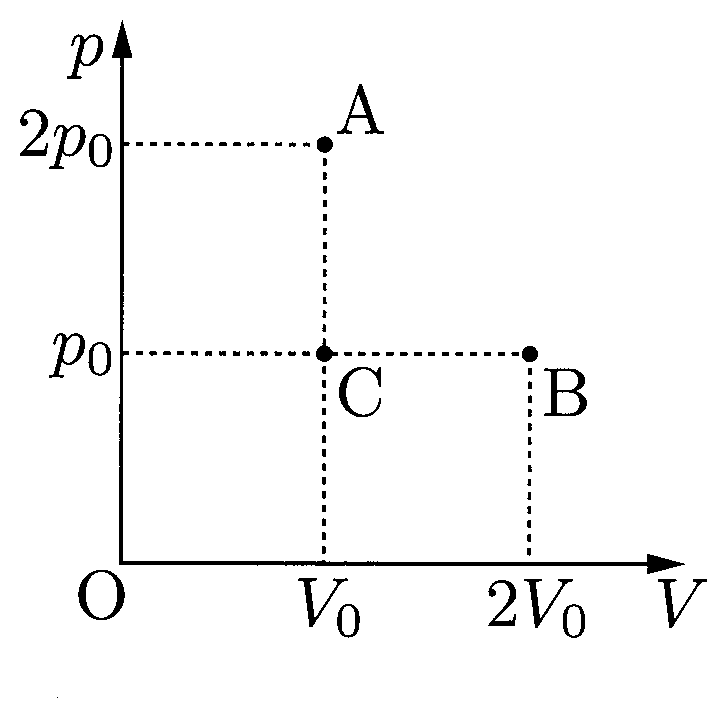
\includegraphics[keepaspectratio,width=34mm]{fig/ch15_p124_pv.png}
\end{center}
\hspace{1zw}各状態変化をそれぞれ考える．
\begin{komon}
\ko{1} $\mathrm{A}\to\mathrm{B}$の状態変化\par
       \hspace*{1zw}この変化において気体の温度は一定であるから，理想気体の状態方程式より，$pV=nRT=$一定となる．よって，体積が$V\U{m^3}$になったときの気体の圧力を$p(V)\U{Pa}$とすれば，$\mathrm{A}$点との間に
       \[p(V)\cdot V=2p_0\cdot V_0\]
       の関係が成立する．よって，
       \[p(V)=2p_0V_0\frac{1}{V}\U{Pa}\quad\left(\propto\frac{1}{V}\right)\]
       となり，$p$-$V$図上では双曲線を描いて変化する．
\ko{2} $\mathrm{B}\to\mathrm{C}$の変化\par
       \hspace*{1zw}この変化途中の，温度，体積がそれぞれ$(T,\ V)$の状態のときの気体の圧力を$p(V)\U{Pa}$とおく．グラフより，体積と温度は
       \[T=\frac{T_0}{V_0}V\]
       の関係を保ちつつ，$T=2T_0\to T_0\U{K}$（$V=2V_0\to V_0\U{m^3}$）まで変化する．また，$(p(V),\ T,\ V)$のときの状態方程式より，
       \[p(V)\cdot V=nRT\]
       が成立するので，以上2式を整理すると，
       \[p(V)=nR\frac{T_0}{V_0}=p_0\]
       となり，変化途中の気体の体積$V$によらず，圧力は常に$p_0\U{Pa}$となる．すなわち，この変化は定圧変化であり，$\mathrm{B}\to\mathrm{C}$へは$p=p_0$の直線上を$V=2V_0\to V_0\U{m^3}$まで変化する．
\ko{3} $\mathrm{C}\to\mathrm{A}$の状態変化\par
       \hspace*{1zw}この変化では，与えられた$T-V$グラフより体積が一定値のまま変化するので，$\mathrm{C}\to\mathrm{A}$へは$V=V_0$の直線上を変化していく．
\end{komon}
\hspace{1zw}以上をまとめると，この状態変化の$p$-$V$図は次図のようになる．
\begin{center}
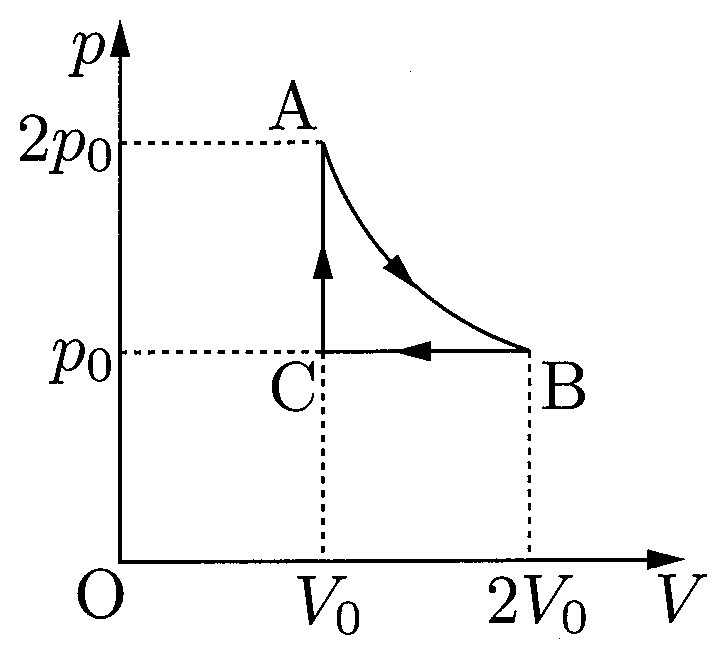
\includegraphics[keepaspectratio,width=34mm]{fig/ch15_p125_pv.png}
\end{center}
\hspace*{\fill}\Ans

\MonN{17}{定圧変化}\par\nopagebreak
\begin{sisin}
気体の状態変化の問題では，初状態と終状態の簡単な図を描き，各々の状態について状態方程式を立て，それぞれのときの圧力，体積，温度の三つを整理しておくと分かりやすい．

一般に，気体の状態変化に関して熱力学第一法則を用いる問題は，\MARU{1}気体が外界にする仕事$W_{\mathrm{out}}$の計算（$p$-$V$図のグラフと$V$軸で囲む面積），\MARU{2} $\Delta U=nC_V\Delta T$の計算，\MARU{3}熱力学第一法則$Q_{\mathrm{in}}=\Delta U+W_{\mathrm{out}}$の立式，という流れに沿うものが多い．この\MARU{2}の$\Delta U=nC_V\Delta T$の計算の際に初状態・終状態の温度が必要になるので，各状態での気体の温度はしっかりと押さえること．なお，$\Delta U=nC_V\Delta T$は定積モル比熱$C_V$を用いているが，この式は\underline{定積変化}\hskip0pt\underline{に限らず}\hskip0pt\underline{あらゆる}\hskip0pt\underline{状態変化}\hskip0pt\underline{に関して}\hskip0pt\underline{成立する}式である．

本問の場合，ピストンが自由に動け，かつゆっくり熱を与える（＝ゆっくりと変化させる）とあるので，ピストンの左右の圧力は常につり合っていると考えられる（いずれかの圧力が高ければ，圧力がつり合うような位置にピストンが移動する）．よって，気体の圧力は常に外圧（大気圧）と等しくなっている．

本問では単原子分子の理想気体であるとは書かれていないので，$C_V=\dfrac{3}{2}R$であるとは限らない．勝手に$C_V=\dfrac{3}{2}R$と置かないようにしよう．
\end{sisin}
\KaiHead
\begin{komon}
\ko{1} ピストンが自由に動け，かつゆっくりと変化させているので，この気体の圧力は常に大気圧$p_0\U{Pa}$に等しい．よって，最初の状態について状態方程式を立てると，
       \[p_0\cdot Sl_0=nRT_0\]
       これより，
       \[p_0=\frac{nRT_0}{Sl_0}\U{Pa}\Ans\]
\ko{2} (1)で述べたように，この気体の圧力は常に大気圧$p_0\U{Pa}$に等しい．加熱により体積は$Sl_1\U{m^3}$に増加するので，終状態の気体の状態方程式を立てると，
       \[p_0\cdot Sl_1=nRT_1\]
       これと(1)の状態方程式を組み合わせて解くと，
       \[T_1=\frac{l_1}{l_0}T_0\U{K}\Ans\]
\ko{3} この気体は圧力を常に大気圧$p_0\U{Pa}$に等しく保って状態変化しているので，この状態変化の$p$-$V$図は次図の通りとなる．
       \begin{center}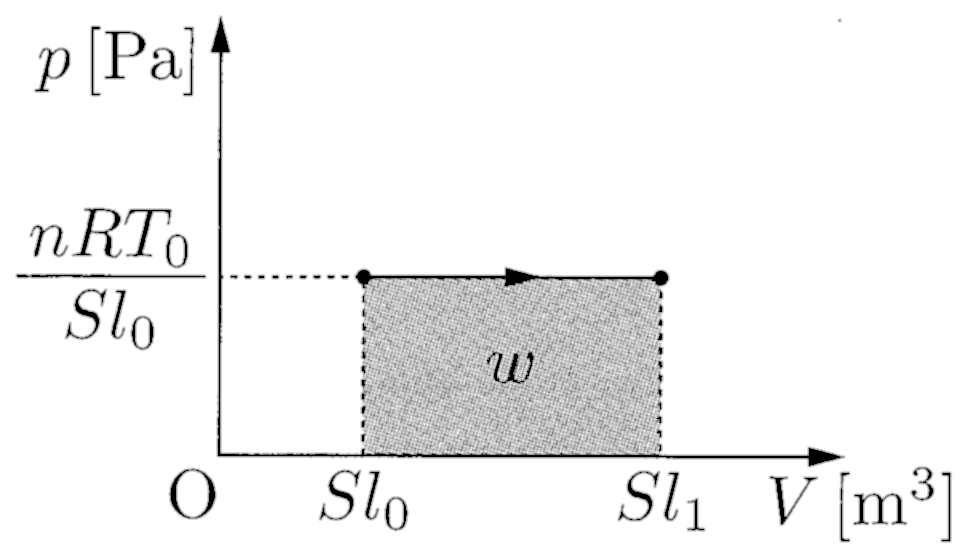
\includegraphics[keepaspectratio,width=58mm]{fig/ch16_a19_pv.png}\end{center}
       \hspace*{\fill}\Ans
\ko{4} この状態変化において気体が外界にした仕事$w\U{J}$は，$Sl_1>Sl_0$ゆえ$p$-$V$図と$V$軸とで囲まれる部分の面積に相当する．よって(3)の$p$-$V$図より，
       \[\begin{aligned}
         w&=\frac{nRT_0}{Sl_0}(Sl_1-Sl_0)\\
          &=nRT_0\left(\frac{l_1}{l_0}-1\right)\U{J}\Ans
       \end{aligned}\]
\ko{5} この状態変化における気体の内部エネルギーの増加量を$\Delta U\U{J}$とすると，
       \[\Delta U=nC_V(T_1-T_0)\]
       と書け，これに(2)の値を代入して計算すると，
       \[\Delta U=nC_VT_0\left(\frac{l_1}{l_0}-1\right)\U{J}\]
       ここで熱力学第一法則より，$\Delta U$, $Q$, $w$の間には
       \[Q=\Delta U+w\]
       の関係が成り立つので，(4)および$\Delta U$を代入して，
       \[Q=n(C_V+R)T_0\left(\frac{l_1}{l_0}-1\right)\U{J}\Ans\]
\end{komon}
\begin{bekkai}
この状態変化は定圧変化であるから，この気体の定圧モル比熱を$C_P$とすると，この状態変化での吸熱量は
\[Q=nC_P\Delta T=nC_P(T_1-T_0)\]
と書き下せる．この気体は理想気体ゆえ，$C_V$と$C_P$の間にはマイヤーの関係式
\[C_P=C_V+R\]
が成立する．よって，
\[\begin{aligned}
  Q&=n(C_V+R)(T_1-T_0)\\
   &=n(C_V+R)T_0\left(\frac{l_1}{l_0}-1\right)\U{J}\Ans
\end{aligned}\]
\end{bekkai}
\begin{chuu}
指針において，$\Delta U=nC_V\Delta T$は\underline{定積変化}\hskip0pt\underline{に限らず}\hskip0pt\underline{あらゆる}\hskip0pt\underline{状態変化}\hskip0pt\underline{に関して}\hskip0pt\underline{成立する}式である，と述べたが，逆に\underline{定圧変化}\hskip0pt\underline{の際にし}\hskip0pt\underline{か成立し}\hskip0pt\underline{ない}式は以下の二つである．
\[Q=nC_P\Delta T,\ w=P\cdot\Delta V\]
この2式は定圧変化以外では利用してはならない．
% 誤植訂正（2026-09-02）：原本は「この2式は定積変化以外では利用してはならない」と
%   なっていたが，直前で「定圧変化の際にしか成立しない式」と述べている．
また，\underline{定積でし}\hskip0pt\underline{か}成立しない式は，
\[Q=nC_V\Delta T\]
である．どの式が一般的に利用できて，どれはできないのかをしっかりと区別すること．
% 誤植訂正（2026-09-02）：原本は「どの式は一般的に利用できて」．
\end{chuu}

\MonN{18}{定積変化}\par\nopagebreak
\begin{sisin}
基本的な流れは前問の定圧変化の場合と全く同じで，\MARU{1}気体が外界にする仕事$W_{\mathrm{out}}$の計算（$p$-$V$図のグラフと$V$軸で囲む面積），\MARU{2} $\Delta U=nC_V\Delta T$の計算，\MARU{3}熱力学第一法則$Q_{\mathrm{in}}=\Delta U+W_{\mathrm{out}}$の立式，という流れに従う．

定積変化の特徴は，体積変化がない$\Rightarrow$気体が仕事をしない，ということである．\underline{気体の仕}\hskip0pt\underline{事のやり}\hskip0pt\underline{取りは気}\hskip0pt\underline{体の体積}\hskip0pt\underline{変化に伴}\hskip0pt\underline{って起こ}\hskip0pt\underline{る}ということを押さえておこう．
\end{sisin}
\KaiHead
\begin{komon}
\ko{1} 初状態も終状態も体積は変わらず$Sl_0\U{m^3}$である．初状態・終状態それぞれについて状態方程式を立てると，
       \[\begin{aligned}
         \text{初状態：}&p_0\cdot Sl_0=nRT_0\\
         \text{終状態：}&p_1\cdot Sl_0=nRT_1
       \end{aligned}\]
       これらを解いて，
       \[p_0=\frac{nRT_0}{Sl_0}\U{Pa},\ p_1=\frac{nRT_1}{Sl_0}\U{Pa}\Ans\]
\ko{2} この状態変化は定積変化であるから，$p$-$V$図上ではグラフは$V$軸に垂直になる．加熱したので$T_1>T_0$であるから，$p_1>p_0$となることに注意すると$p$-$V$図は次図の通り．
       \begin{center}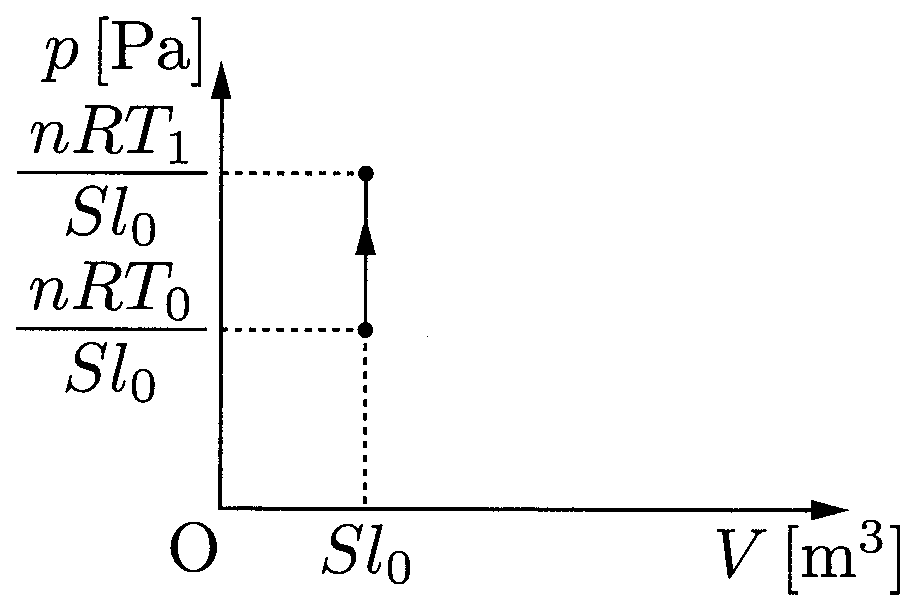
\includegraphics[keepaspectratio,width=52mm]{fig/ch16_a20_pv.png}\end{center}
       \hspace*{\fill}\Ans
\ko{3} この状態変化は定積変化であるから，気体は外界に対して仕事をしない（(2)で，$p$-$V$グラフと$V$軸が囲む面積が0）．よって，
       \[w=0\U{J}\Ans\]
\ko{4} この状態変化における気体の内部エネルギーの増加量を$\Delta U\U{J}$とすると，
       \[\Delta U=nC_V(T_1-T_0)\ \cdots\mbox{（☆）}\]
       と書ける．\par
       \hspace*{1zw}ここで熱力学第一法則より，$\Delta U$, $Q$, $w$の間には
       \[Q=\Delta U+w\]
       の関係が成り立つので，(3)および$\Delta U$を代入して，
       \[Q=nC_V(T_1-T_0)\U{J}\Ans\]
\end{komon}
\begin{bekkai}
この状態変化は定積変化であるから，定積モル比熱の定義より，
\[\begin{aligned}
  Q&=nC_V\Delta T\\
   &=nC_V(T_1-T_0)\U{J}\Ans
\end{aligned}\]
としてもよい．
\end{bekkai}

\Rank{C問題}
\MonN{19}{球内での気体分子運動論}\par\nopagebreak
\begin{sisin}
考え方の指針は直方体容器の場合と全く変わらない．\MARU{1}1回あたりの衝突で壁面に与える力積を求める，\MARU{2}時間$t\U{s}$間での衝突回数および与える力積を求める，\MARU{3}力積と力の関係，および全分子について与える力積を考えて，壁面に作用する力を求める，\MARU{4}気体分子運動の等方向性を利用，\MARU{5}圧力を計算する，という流れである．（本問の場合はすべての分子が同じ速さと考えて分子ごとのバラつきを考えていないため，\MARU{4}は不要）
\end{sisin}
\KaiHead
% 誤植訂正（2026-08-31）：原本の解答は (1)(2) の次が (1)(2)(3)…(7) と振り直されており，
%   問題文の空欄番号（1〜9）と2つずれていた．空欄番号に合わせて (3)〜(9) に改めた．
\begin{komon}
\item[{\makebox[1.9zw][r]{(1)(2)}}] 分子と壁との衝突は完全弾性衝突であるから，衝突前後で点$\mathrm{B}$における接線方向，すなわち半径$\mathrm{OB}$に垂直な方向の速度成分は変化せず，$\mathrm{OB}$方向の速度成分が反転して$v\cos\theta$から$-v\cos\theta$へ変化する．よって，衝突によるこの分子の運動量の変化は，$\mathrm{O}$から$\mathrm{B}$の方向を正として，
       \[m\cdot(-v\cos\theta)-m\cdot v\cos\theta=-2mv\cos\theta\]
       となる．よって，(1)$\ \overrightarrow{\mathrm{BO}}$ベクトルの方向に，大きさ(2)$\ 2mv\cos\theta\U{N\cdot s}$\Ans
\ko{3} 次の衝突点は$\mathrm{C}$であるが，$\mathrm{B}$点での衝突は弾性衝突であるから，$\angle\mathrm{ABO}=\angle\mathrm{OBC}=\theta$である．よって，$\mathrm{B}\to\mathrm{C}$までの距離は，図より
       \[\overline{\mathrm{BC}}=2a\cos\theta\U{m}\]
       である．また，分子の速さは衝突前後で変化しないので，次に衝突するまでにかかる時間は
       \[\frac{\overline{\mathrm{BC}}}{v}=\frac{2a\cos\theta}{v}\U{s}\Ans\]
\ko{4} 図より明らかに$\angle\mathrm{BOC}=\theta$であるから，分子の器壁への入射角は一定である．また，分子の速さも器壁と何回衝突しても一定のままであるから，衝突時間間隔はずっと$\dfrac{2a\cos\theta}{v}\U{s}$の一定のままである．よって，時間$t\U{s}$間の間の壁面との衝突回数は
       \[t\Big/\frac{2a\cos\theta}{v}=\frac{vt}{2a\cos\theta}\,[\text{回}]\Ans\]
\ko{5} 一回の衝突によってこの気体分子が壁面に対して与える力積の大きさは，(1)・(2)の正負逆なので
       \[\text{壁面を押す方向に，大きさ}\ 2mv\cos\theta\U{N\cdot s}\]
       である．よって，時間$t\U{s}$間の間に壁面に対して与えた力積の大きさの総和は
       \[2mv\cos\theta\cdot\frac{vt}{2a\cos\theta}=\frac{mv^2}{a}t\U{N\cdot s}\Ans\]
\ko{6} 1分子あたりが(5)であるから，
       \[N\cdot\frac{mv^2}{a}t\U{N\cdot s}\Ans\]
\ko{7} 器壁に及ぼす平均の力の大きさを$\overline{F}\U{N}$とすれば，平均の力と力積との関係より，
       \[\overline{F}\cdot t=N\cdot\frac{mv^2}{a}t\]
       である．よって，器壁に対して及ぼす平均の力の大きさは
       \[\overline{F}=\frac{Nmv^2}{a}\U{N}\Ans\]
\ko{8} 容器内面の面積は$S=4\pi a^2\U{m^2}$であるから，
       \[p=\frac{\overline{F}}{S}=\frac{\dfrac{Nmv^2}{a}}{4\pi a^2}=\frac{Nmv^2}{4\pi a^3}\U{Pa}\Ans\]
\ko{9} また$V=\dfrac{4}{3}\pi a^3\U{m^3}$より，
       \[p=\frac{Nmv^2}{3V}\]
       よって，
       \[pV=\frac{Nmv^2}{3}\Ans\]
\end{komon}
\begin{bsHosoku}{参考}
結局，球形の容器であっても気体分子の速さの二乗と圧力との関係式は，立方体容器の場合と全く同一になる．また，これと状態方程式を組み合わせれば気体の二乗平均速度の式が立方体容器の場合と全く同様に導かれる．
\end{bsHosoku}
\begin{bsHosoku}{参考}
（ここに書かれていることはかなり難しいため，興味のある人のみ読めばよい）\par
\hspace*{1zw}本問では気体分子運動の等方向性
\[\overline{v_x^2}=\overline{v_y^2}=\overline{v_z^2}\]
を利用しなかったが，この式は容器の形状によらずに成立する．\par
\hspace*{1zw}これは気体分子同士が非常に頻繁に相互に衝突しているためである．例えば$0\Cel$，1気圧下において，気体分子が他の気体分子に衝突せずに進める距離（平均自由行程という）はおよそ$10^{-7}\U{m}$程度でしかなく，およそ$10^{-19}\U{s}$程度の間隔で気体分子は衝突を繰り返している．
このため，例えば容器の一部の器壁などの移動によってある軸方向の速度成分が大きくなったとしても，気体分子相互の衝突のためすぐに他の軸方向の速度成分も増加してしまう（断熱変化を気体分子運動論に基づいて考える場合などに用いられる）．\par
\hspace*{1zw}ベルヌーイの式の導出などに用いた「気体分子相互の衝突はない」という仮定とつじつまが合わなくなってしまうように感じるかもしれないが，これについては考慮しなくてよい．というのは，本来ベルヌーイの式は統計熱力学を元にして導出されるものであり，これを高校範囲の知識だけで扱おうとするのは無理である．正しくはどうなのか，という点については大学に入ってから学べばよいが，高校範囲では次のように考えて問題を解けばよい．
\begin{komon}
\item[{\makebox[1.9zw][r]{\MARU{1}}}] ベルヌーイの式を導く際には，気体分子相互間の衝突については考慮しなくてよい．
\item[{\makebox[1.9zw][r]{\MARU{2}}}] ただし，気体分子運動の等方向性を用いる際には，気体分子の相互衝突が起こっていると考える．
\end{komon}
\end{bsHosoku}

\MonN{20}{定積・定圧変化}\par\nopagebreak
\begin{sisin}
最初の状態ではストッパーに支えられているので，内部の気体がピストンに及ぼす上向きの力の方が，ピストンに対してかかる下向きの力（重力，大気圧による力）よりも小さければピストンは動き出さない．気体を加熱して内圧を上昇させ，上向きの力が下向きの力を上回ったとき初めて動き出す．よって，ピストンが動き出すまでの間は，ピストンに作用する外圧$P_0S$，内圧$PS$，重力$Mg$の三つはつり合ってはいない．このことに注意して考えよ．
\end{sisin}
\KaiHead
\begin{komon}
\ko{1} 初めの状態について，気体の状態方程式を立てると，
       \[p'(Sl_0)=nRT_0\]
       であるから，
       \[p'=\frac{nRT_0}{Sl_0}\U{Pa}\Ans\]
\ko{2} 気体の内圧を$P$とすると，このピストンに対しては図のように力が作用している．
       \begin{center}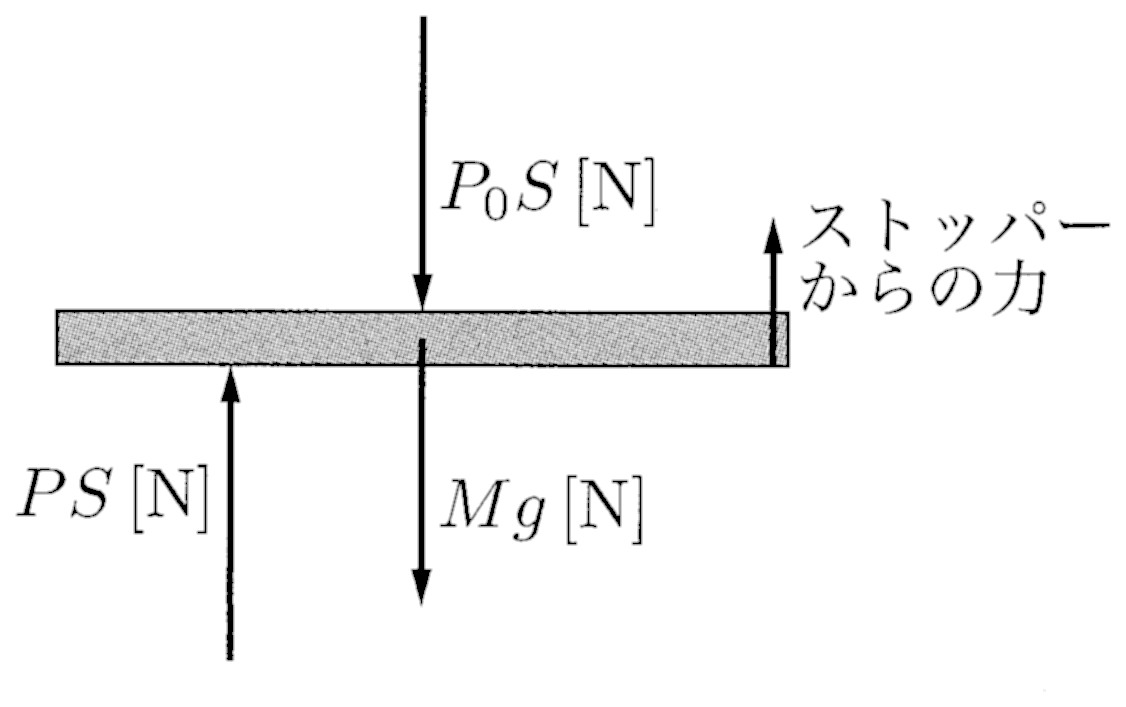
\includegraphics[keepaspectratio,width=66mm]{fig/ch16_a23_f1.png}\end{center}
       ピストンが上昇しはじめるのはストッパーが支える力がなくなったとき，すなわち，
       \[PS\geqq P_0S+Mg\]
       の条件が満たされるようになったときである．ゆえに，このときの気体の圧力$P_1$は
       \[P_1=P_0+\frac{Mg}{S}\U{Pa}\]
       である．この瞬間の気体の体積はまだ$Sl_0\U{m^3}$であることに注意して状態方程式を立てると，
       \[P_1(Sl_0)=nRT_1\]
       であるから，これを解いて，
       \[T_1=\frac{(P_0S+Mg)l_0}{nR}\U{K}\Ans\]
\ko{3} 一旦ピストンが上昇をはじめると，ピストンにはたらく力の関係はもう変わらないため，気体の圧力は
       \[P_1=P_0+\frac{Mg}{S}\U{Pa}\]
       のまま一定となり，定圧変化を続ける．終状態についても気体の圧力はこの$P_1$であるから，終状態についての状態方程式を立てると，
       \[P_1(Sl_1)=nRT_2\]
       であるから，これを解いて，
       \[T_2=\frac{(P_0S+Mg)l_1}{nR}\U{K}\Ans\]
\ko{4} \MARU{1}ピストンが動き始めるまでの間についてと，\MARU{2}ピストンが動き始めてから，とに分けて考える．\par
       \hspace*{1zw}\MARU{1}については気体は定積変化をしているので，この間に気体がした仕事$w_1$は0であり，内部エネルギー変化$\Delta U_1$は，
       \[\Delta U_1=nC_V(T_1-T_0)\]
       である．よってこの間の吸熱量$Q_1$は，熱力学第一法則より，
       \[Q_1=\Delta U_1+w_1=nC_V(T_1-T_0)\]
       である．また，\MARU{2}については気体は定圧変化をしているので，この間に気体がした仕事$w_2$は
       \[w_2=P_1\cdot\Delta V=P_1\cdot S(l_1-l_0)\]
       であり，内部エネルギー変化$\Delta U_2$は
       \[\Delta U_2=nC_V(T_2-T_1)\]
       である．よってこの間の吸熱量$Q_2$は，熱力学第一法則より，
       \[\begin{aligned}
         Q_2&=\Delta U_2+w_2\\
            &=nC_V(T_2-T_1)+P_1\cdot S(l_1-l_0)
       \end{aligned}\]
       である．以上より，気体に与えられた総熱量は，
       \[\begin{aligned}
         Q&=Q_1+Q_2\\
          &=nC_V(T_1-T_0)+nC_V(T_2-T_1)\\
          &\hspace*{\fill}+P_1\cdot S(l_1-l_0)\\
          &=\frac{C_V+R}{R}(P_0S+Mg)l_1-nC_VT_0\\
          &\hspace*{\fill}-(P_0S+Mg)l_0\U{J}\Ans
       \end{aligned}\]
\end{komon}
\begin{bekkai}
\MARU{2}についてはマイヤーの関係式$C_P=C_V+R$を用いて考えてもよい．
\[\begin{aligned}
  Q_2&=nC_P(T_2-T_1)\\
     &=n(C_V+R)(T_2-T_1)
\end{aligned}\]
であるから，
\[\begin{aligned}
  Q&=Q_1+Q_2\\
   &=nC_V(T_1-T_0)\\
   &\hspace*{\fill}+n(C_V+R)(T_2-T_1)\\
   &=nC_V(T_2-T_0)+nR(T_2-T_1)\\
   &=n(C_V+R)T_2-nC_VT_0-nRT_1
\end{aligned}\]
と変形して同じ答えを得る．

また，状態変化全体に対して熱力学第一法則を利用するのも手である．\MARU{1}＋\MARU{2}を一つの変化だとみなすと，この間の内部エネルギー変化は
\[\Delta U=nC_V(T_2-T_0)\]
であり，気体が外にした仕事は\MARU{2}のときの
\[w_2=P_1\cdot\Delta V=P_1\cdot S(l_1-l_0)\]
である．これと熱力学第一法則を組み合わせても同じ答えが得られる．
% 誤植訂正（2026-09-02）：原本はこの式を $w_1$ としているが，\MARU{2} の区間の仕事は
%   本解で $w_2$ と置いている（$w_1=0$）．
\end{bekkai}

\MonN[\Sitei]{21}{断熱変化における気体分子運動論}\par\nopagebreak
\begin{sisin}
断熱変化におけるポアソンの式（第23回で扱う）を，気体分子運動という微視的な観点から導出する問題である．基礎講座の問題としては難問であるが，ぜひこの機会に方針を覚えておいてほしい．\par
\hspace*{1zw}$pV=Nk_{\mathrm{B}}T$は気体の状態方程式$pV=nRT$を書き換えた式である．アボガドロ数を$N_{\mathrm{A}}$とすると$n=\dfrac{N}{N_{\mathrm{A}}}$であるから，
\[nR=\frac{N}{N_{\mathrm{A}}}R=N\frac{R}{N_{\mathrm{A}}}=Nk_{\mathrm{B}}\]
と書き換えられる．\par
\hspace*{1zw}本問のキーポイントは(6)および(10)にある．(6)では，ピストンが動いているので，衝突後における分子の速度の$x$成分は$-v_x$とはならない．衝突の前後をピストン上から見て，はね返り係数の定義式を利用する．\par
\hspace*{1zw}(10)については以下のように考えると分かりやすいだろう．気体分子は実際には多数回，他の分子と衝突を繰り返しており，気体分子は$x, y, z$軸方向にランダムに飛び交っている．その結果，各軸方向の速さの2乗の平均はすべて等しくなり，$\overline{v_x^2}=\overline{v_y^2}=\overline{v_z^2}$が常に成立する．\par
\hspace*{1zw}そのため，$x$軸方向に気体を圧縮することで$x$軸方向の運動エネルギー$\dfrac{1}{2}m\overline{v_x^2}$を増加させても，気体分子間の衝突により$\overline{v_x^2}=\overline{v_y^2}=\overline{v_z^2}$が満たされるように，$x$軸方向の運動エネルギーが減り，その分，$y, z$軸方向の運動エネルギーが増加する．$x$軸方向に気体を圧縮することで気体分子に与えられたエネルギーが$E$であれば，各軸方向の運動エネルギーの増加の総和が$E$になるので，
\[\begin{aligned}
&\Delta\left(\frac{1}{2}m\overline{v_x^2}\times N\right)+\Delta\left(\frac{1}{2}m\overline{v_y^2}\times N\right)\\
&\hspace*{6mm}+\Delta\left(\frac{1}{2}m\overline{v_z^2}\times N\right)=E
\end{aligned}\]
が成立する．これと気体分子運動の等方向性を併せることで(10)が導ける．
\end{sisin}
\KaiHead
\begin{komon}
\ko{1} 分子とピストンとの衝突は完全弾性衝突であるから，衝突前後でこの分子の速度は$x$成分のみが$v_x$から$-v_x$へ変化する．よって衝突による分子の運動量の変化は，
       \[m\begin{pmatrix}-v_x\\ v_y\\ v_z\end{pmatrix}-m\begin{pmatrix}v_x\\ v_y\\ v_z\end{pmatrix}=\begin{pmatrix}-2mv_x\\ 0\\ 0\end{pmatrix}\]
       であり，これは衝突時に気体分子がピストンから受けた力積である．ここで作用・反作用の関係より，分子がピストンに及ぼした力積はこれと正負逆の関係になるので，その大きさは
       \[2mv_x\U{N\cdot s}\Ans\]
\ko{2} ピストンに衝突した後，分子が$x$軸方向に$2l\U{m}$の道のりを進んで往復すると再びピストンに衝突する．一往復には時間$\dfrac{2l}{v_x}\U{s}$を要するので，$1\U{s}$間あたりにピストンと衝突する回数は，
       \[1\Big/\frac{2l}{v_x}=\frac{v_x}{2l}\,[\text{回}]\Ans\]
\ko{3} (1)および(2)より，
       \[2mv_x\cdot\frac{v_x}{2l}=\frac{mv_x^2}{l}\U{N\cdot s}\Ans\]
\ko{4} 気体の圧力を$p\U{Pa}$とすると，気体の圧力がピストンに及ぼす$1\U{s}$あたりの力積は，
       \[pS\times 1\U{N\cdot s}\]
       である．気体の圧力の正体は，気体の全分子のピストンへの衝突であるから，
       \[pS\times 1=\frac{m\overline{v_x^2}}{l}\times N\]
       である．これを解いて，
       \[p=\frac{Nm\overline{v_x^2}}{Sl}\U{Pa}\Ans\]
\ko{5} (4)を書き換えると，
       \[pSl=Nm\overline{v_x^2}\]
       である．気体の状態方程式は$pSl=Nk_{\mathrm{B}}T$であるから，2式を比較して，
       \[\overline{v_x^2}=\frac{k_{\mathrm{B}}T}{m}\Ans\]
\ko{6} 衝突後の速度の$x$成分を$v_x'\U{m/s}$とすると，ピストンから見た跳ね返り前後の速さは次図のようになる．
       \begin{center}
       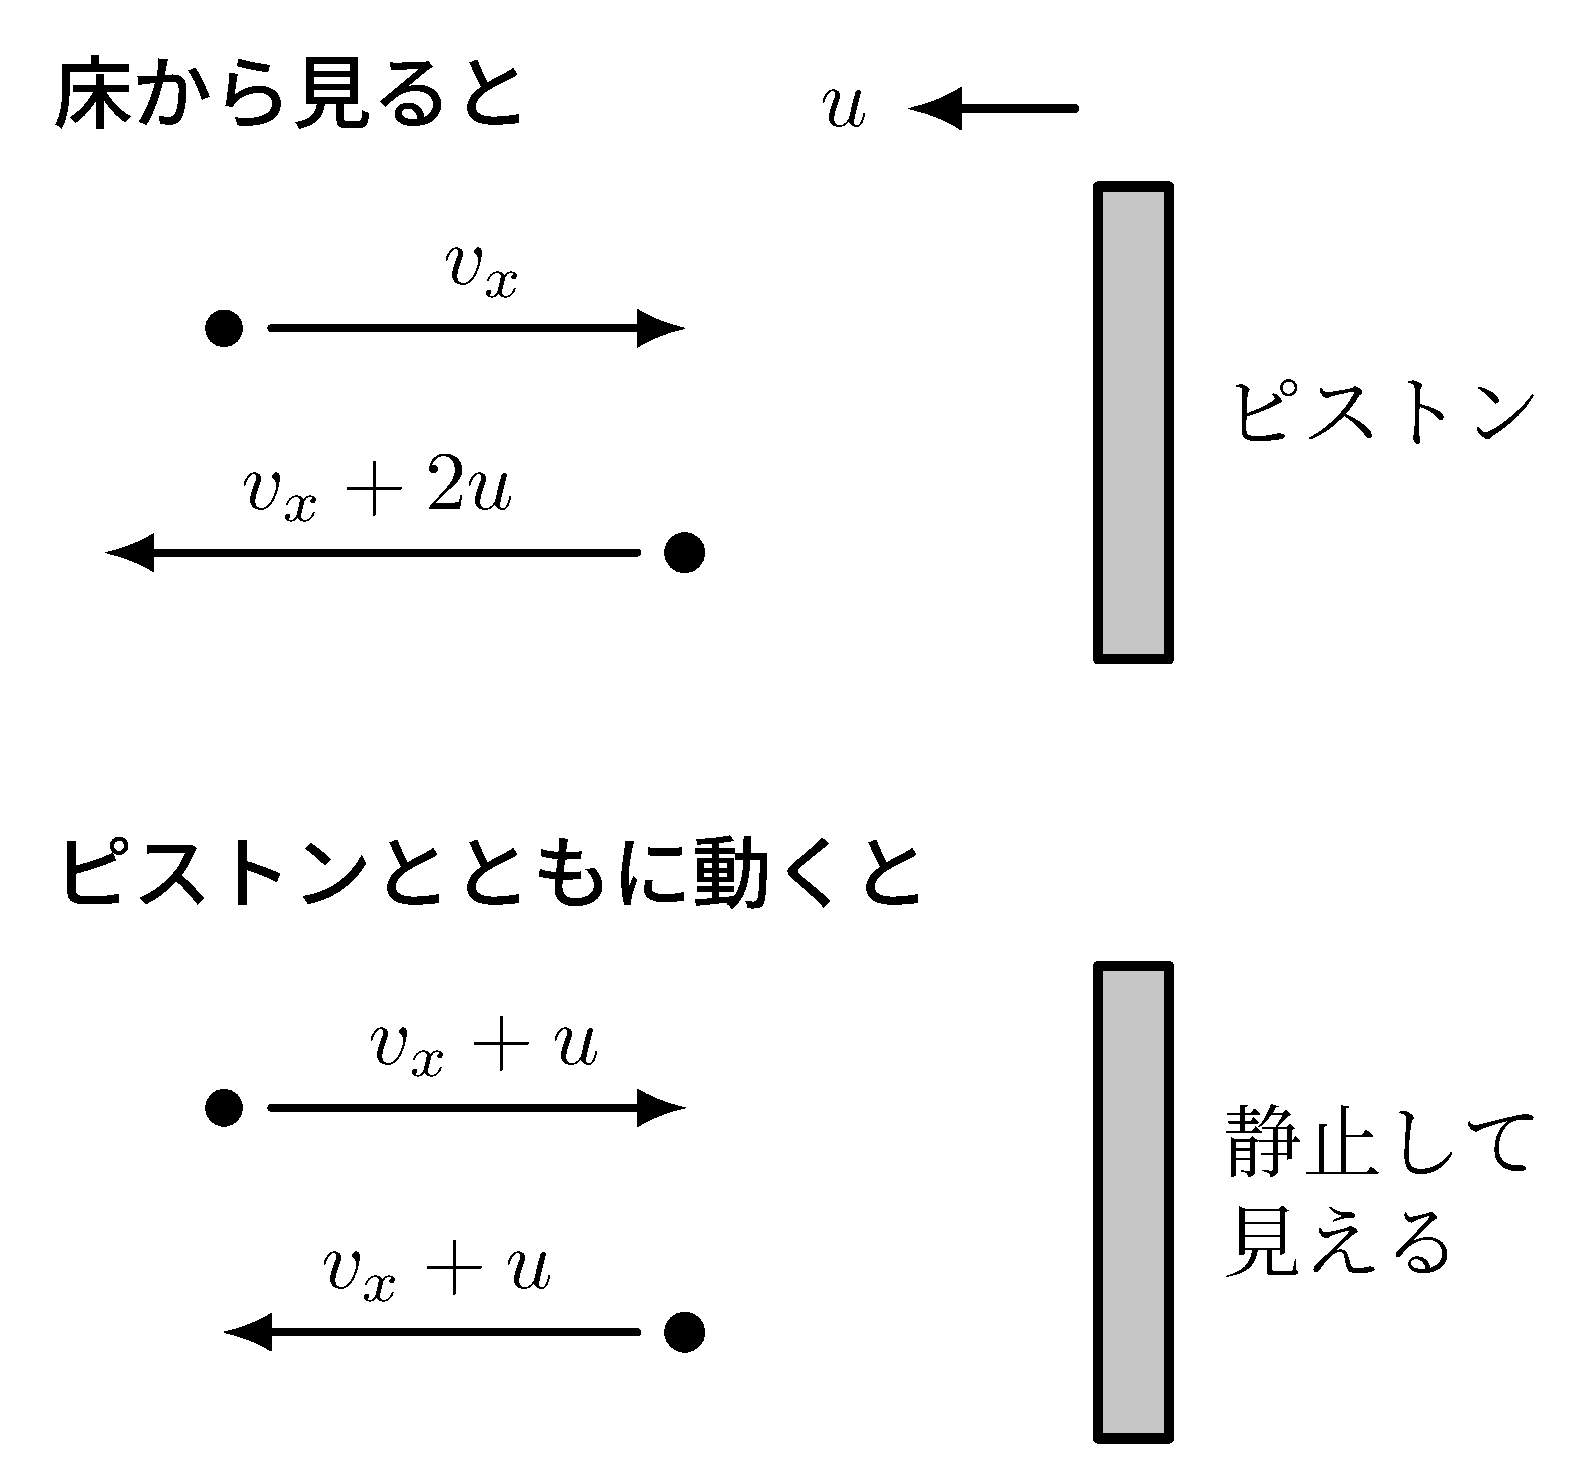
\includegraphics[keepaspectratio,width=62mm]{fig/n22_zu_kabe.png}
       \end{center}
       弾性衝突だからピストンから見た速さは衝突の前後で変わらず，床から見た速さに直すには$u$を足せばよい，と考えてもよい．式で書くと，はね返り係数が1なので，
       \[1=-\frac{v_x'-(-u)}{v_x-(-u)}\]
       これを解いて，$v_x'=-(v_x+2u)$である．よって，衝突後の$x$方向の速さは，
       \[|v_x'|=v_x+2u\U{m/s}\Ans\]
\ko{7} (6)より，
       \[\begin{aligned}
         |v_x'|^2-v_x^2&=(v_x+2u)^2-v_x^2\\
                       &=4uv_x+4u^2
       \end{aligned}\]
       ここで，第1項$4uv_x$は1次微小項（微小量$u$の1次の項），第2項$4u^2$は2次微小項であるから，第1項に比べて第2項は無視できる．よって，一次近似（$=$1次微小項までを取る）を行うと，
       \[4uv_x+4u^2\fallingdotseq 4uv_x\U{m^2/s^2}\Ans\]
\end{komon}
\begin{bsHosoku}{参考}
一般に，1次微小項に対して2次微小項は無視でき，2次微小項に比べて3次微小項は無視できる．
\end{bsHosoku}
\begin{komon}
\ko{8} $\Delta l\ll l$であるから，往復距離は$2l\U{m}$とみなしてよく，また$u\ll v_x$であるから往復する速さは$v_x$とみなしてよい．よって，一往復に要する時間は
       \[\frac{2l}{v_x}\U{s}\quad\cdots\text{☆}\]
       とみなしてよい．ピストンが距離$\Delta l\U{m}\ (\ll l)$だけ動くのに要する時間は$\dfrac{\Delta l}{u}\U{s}$であるから，この間に分子がピストンに衝突する回数は
       \[\frac{\Delta l}{u}\Big/\frac{2l}{v_x}=\frac{v_x\Delta l}{2ul}\,[\text{回}]\Ans\]
\end{komon}
\begin{chuu}
☆は，(6)で計算した$x$軸方向の速さの変化$2u$を無視してよい，ということであるが，\underline{$2u$その}\hskip0pt\underline{ものが}\hskip0pt\underline{ないと}\hskip0pt\underline{考えて}\hskip0pt\underline{よい}\hskip0pt\underline{という}\hskip0pt\underline{ことで}\hskip0pt\underline{はない}ことに注意せよ．上の参考で述べたように，より高次の微小量は無視することができる．ピストンと$n$回衝突することにより，その速さは$v_x+2nu\U{m/s}$となるが，$v_x$（0次微小項）に比べて$2nu$（1次微小項）は無視できる．よって，$x$軸方向の速さを$v_x$とみなして往復時間を求めてよいのである（往復距離を$2l$とみなしてよいのも全く同様である）．\par
\hspace*{1zw}これに対して，(7)で1次微小量$2u$がないと考えてしまうと，$|v_x'|^2-v_x^2\fallingdotseq 0$となってしまい，これは明らかにおかしい．このようになってしまったら，近似が粗すぎるということを意味する．このような場合は，より高次の微小量まで入れて計算してから，最も次数の低い微小量のみを残して残りを切り捨てることにより，近似計算を行う．
\end{chuu}
\begin{komon}
\ko{9} (7), (8)より，
       \[4uv_x\cdot\frac{v_x\Delta l}{2ul}=\frac{2v_x^2\Delta l}{l}\U{m^2/s^2}\Ans\]
\ko{10} これにより，$x$軸方向の二乗の平均値$\overline{v_x^2}$は$\overline{v_x^2}+\dfrac{2\overline{v_x^2}\Delta l}{l}$に増加するので，分子の平均運動エネルギーは
       \[\frac{1}{2}m\left(\overline{v_x^2}+\frac{2\overline{v_x^2}\Delta l}{l}\right)-\frac{1}{2}m\overline{v_x^2}=\frac{m\overline{v_x^2}\Delta l}{l}\]
       だけ増加する．しかし実際には，気体分子の相互衝突により$x, y, z$方向の速さの二乗の平均値が等しくなるように，すべての軸方向の運動エネルギー（二乗の平均値）が等しく増加するので，
       \[\begin{aligned}
         &\Delta\left(\frac{1}{2}m\overline{v_x^2}\right)+\Delta\left(\frac{1}{2}m\overline{v_y^2}\right)+\Delta\left(\frac{1}{2}m\overline{v_z^2}\right)\\
         &\hspace*{16mm}=3\times\Delta\left(\frac{1}{2}m\overline{v_x^2}\right)
       \end{aligned}\]
       が成立する．よって，
       \[3\times\Delta\left(\frac{1}{2}m\overline{v_x^2}\right)=\frac{m\overline{v_x^2}\Delta l}{l}\]
       となる．すなわち，実際の$x$軸方向の運動エネルギー増加はピストン圧縮で与えられたエネルギーの$\dfrac{1}{3}$であり，
       \[\Delta\left(\frac{1}{2}m\overline{v_x^2}\right)=\frac{m\overline{v_x^2}\Delta l}{3l}\]
       である（残り$\dfrac{2}{3}$は$y, z$軸方向の運動エネルギー増加に利用される）．よって，$x$方向の速度の二乗の平均値の増加量$\Delta\left(\overline{v_x^2}\right)\U{m^2/s^2}$は，
       \[\Delta\left(\overline{v_x^2}\right)=\frac{2\overline{v_x^2}}{3l}\Delta l\U{m^2/s^2}\Ans\]
\end{komon}
\begin{chuu}
上述の答案の，$\Delta(\ \ )$という表記は，$(\ \ )$内の物理量の増分を表す．
\end{chuu}
\begin{komon}
\ko{11} (5)の関係式より，$\overline{v_x^2}+\Delta\left(\overline{v_x^2}\right)=\dfrac{k_{\mathrm{B}}}{m}(T+\Delta T)$と$\overline{v_x^2}=\dfrac{k_{\mathrm{B}}}{m}T$が成り立つが，辺々引いて，$x$方向の速度の二乗の平均値の増加量$\Delta\left(\overline{v_x^2}\right)\U{m^2/s^2}$と温度上昇$\Delta T\U{K}$の間には，
       \[\Delta\left(\overline{v_x^2}\right)=\frac{k_{\mathrm{B}}}{m}\Delta T\]
       が成立する．よって，
       \[\Delta T=\frac{2m\overline{v_x^2}}{3k_{\mathrm{B}}l}\Delta l\U{K}\]
       である．さらに(5)の関係式を利用して$\overline{v_x^2}$を$T$で書き換えると，
       \[\Delta T=\frac{2}{3}T\cdot\frac{\Delta l}{l}\U{K}\Ans\]
\end{komon}
\begin{bsHosoku}{参考}
さらに上で得られた式を変形すると，
\[\Delta T=\frac{2}{3}T\cdot\frac{S\Delta l}{Sl}=-\frac{2}{3}T\frac{\Delta V}{V}\]
となる．ここまでで考えてきた変化は微小変化であるから，$\Delta V$を$dV$で，また$\Delta T$を$dT$で置き換えてよく，
\[dT=-\frac{2}{3}T\cdot\frac{dV}{V}\]
と書ける．両辺に変数を分離すると，
\[\frac{dT}{T}=-\frac{2}{3}\cdot\frac{dV}{V}\]
であり，両辺を積分すると
\[\int\frac{dT}{T}=-\frac{2}{3}\int\frac{dV}{V}\]
であるから，
\[\log_e|T|=-\frac{2}{3}\log_e|V|+C\]
である．これを変形すると，
\[\log_e|T|+\log_e\left|V^{\frac{2}{3}}\right|=C\]
より，
\[TV^{\frac{2}{3}}=(\text{一定})\]
という，単原子分子理想気体の場合のポアソンの式が導かれる．
\end{bsHosoku}

\end{multicols}
